% Initial version by Darian Muresan, Ph.D.
% Edit and adjust as needed.

\documentclass[12pt]{cornell}

% add index support
\makeindex

% graphing programs
\usepackage{color}
\usepackage{psfrag}
\usepackage{verbatim}
\usepackage{fancyhdr}
%\usepackage{titlesec}
\usepackage{fancyvrb} 
% hyperlink programs
\usepackage[pdfmark, 
breaklinks=true, 
colorlinks=true,
citecolor=blue,
linkcolor=blue,
menucolor=black,
pagecolor=black,
urlcolor=blue
]{hyperref} % links in pdf
%\usepackage[colorlinks]{hyperref} % links in dvi
\usepackage{listings}
\usepackage{amsfonts} 
\usepackage{amssymb} 
%\usepackage{tabto}

\usepackage{tabularx,colortbl}
\usepackage[chapter]{algorithm} 
\usepackage{algorithmic} 
\usepackage{blindtext}
\usepackage{imakeidx}


\definecolor{DarkGreen}{rgb}{0,0.6,0}
\definecolor{mygreen}{rgb}{0,0.6,0}
\definecolor{mygray}{rgb}{0.5,0.5,0.5}
\definecolor{mymauve}{rgb}{0.58,0,0.82}

\usepackage{tocloft}
\usepackage{amsmath}
\usepackage{tcolorbox}
\usepackage{enumitem}
\usepackage{longtable}
%\usepackage{textcomp}
\usepackage{txfonts}

%part for \part titles
%chap for \chapter titles
%sec for \section titles
%subsec for \subsection titles
%subsubsec for \subsubsection titles
%para for \paragraph titles
%subpara for \subparagraph titles
%fig for figure \caption titles
%subfig for subfigure \caption titles
%tab for table \caption titles
%subtab for subtable \caption titles

% update chapter number spacing
\setlength{\cftchapnumwidth}{2em}
\setlength{\cftsecnumwidth}{2.5em}
\setlength{\cftsubsecnumwidth}{3.5em}
\setlength{\cftsubsubsecnumwidth}{4.5em}

\addtolength{\cftsecindent}{0.5em}
\addtolength{\cftsubsecindent}{0.5em}
\addtolength{\cftsubsubsecindent}{0.5em}

%\titlespacing*{\chapter}{0pt}{-50pt}{20pt}
%\titleformat{\chapter}[display]{\normalfont\huge\bfseries}{\chaptertitlename\ 
%\thechapter}{20pt}{\Huge}
%\pagestyle{fancy}
%\pagestyle{cornell}
%
%\rhead{F054-021-0172}
%\chead{Nonlinear Enhancement of Visual Target Detection (AF05-T021)}
%\lhead{GSTI}
%\lfoot{\scriptsize Use or disclosure of data on this page is subject
%to the restriction on the title page of this proposal.}
%\cfoot{}
%\rfoot{\thepage}

\newfont{\Bp}{msbm10}
\newfont{\BpBig}{msbm10 scaled\magstep2}
\newfont{\Sc}{eusm10}
\newfont{\ScBig}{eusm10 scaled\magstep3}
\newfont{\Fr}{eufm10}
\newfont{\FrBig}{eufm10 scaled\magstep1}

% some commands:
\newcommand{\dxi}{{\tt m\_xDeltaInput}}
\newcommand{\dyi}{{\tt m\_yDeltaInput}}
\newcommand{\dci}{{\tt m\_cDeltaInput}}
\newcommand{\dxo}{{\tt m\_xDeltaOutput}}
\newcommand{\dyo}{{\tt m\_yDeltaOutput}}
\newcommand{\dco}{{\tt m\_cDeltaOutput}}
\newcommand{\ttf}[1]{{\tt #1}}
\newcommand{\tbl}[2]{{\begin{tabular}{c} #1 \\ #2 \end{tabular}}}

\newcommand{\urltwo}[2]{\mbox{\href{#1}{\tt #2}}}
\newcommand{\qnorm}[1]{\|#1\|_{\bQ}}
\newcommand{\qdot}[2]{\lrb #1, #2 \rrb_{\bQ}}
\newcommand{\kdot}[2]{\lrb #1, #2 \rrb_{\bf k}}
\newcommand{\tdot}[2]{\lrb #1, #2 \rrb}
\newcommand{\mydiff}[2]{\lrb #1 - #2 \rrb}
\newcommand{\lena}{\textit{lena}}
\newcommand{\barb}{\textit{barbara}}
\newcommand{\boat}{\textit{boat}}
\newcommand{\leaves}{\textit{leaves}}
\newcommand{\rings}{\textit{rings}}
\newcommand{\treg}{\textit{train region}}
\newcommand{\dreg}{\textit{denoise region}}
\newcommand{\oreg}{\textit{overlap region}}
\newcommand{\sil}{\sigma_l^2}
\newcommand{\sn}{\sigma^2}
\newcommand{\bn}{{\mbox{\bf \FrBig N}}}
\newcommand{\n}{\mbox{\Fr N}}
%\newcommand{\bn}{\bf N}
%\newcommand{\n}{N}
\newcommand{\bY}{\textbf{Y}}
\newcommand{\bX}{\textbf{X}}
\newcommand{\bb}{\textbf{b}}
\newcommand{\bu}{\textbf{u}}
\newcommand{\bv}{\textbf{v}}
\newcommand{\by}{\textbf{y}}
\newcommand{\bx}{\textbf{x}}
\newcommand{\be}{\textbf{e}}
\newcommand{\bz}{\textbf{z}}
\newcommand{\bs}{\textbf{s}}
\newcommand{\bw}{\textbf{w}}
\newcommand{\bQ}{\textbf{Q}}
\newcommand{\bphi}{\textbf{$\phi$}}
\newcommand{\lsb}{\left[}
\newcommand{\rsb}{\right]}
\newcommand{\lrb}{\left(}
\newcommand{\rrb}{\right)}
\newcommand{\lcb}{\left\{}
\newcommand{\rcb}{\right\}}
\newcommand{\R}{\mbox{\BpBig R}}
\newcommand{\F}{{\cal F}}
\newcommand{\Fk}{\mbox{\Sc F}}
\newcommand{\bQF}{\textbf{Q}_{\mbox{\Sc F}}}
\newcommand{\N}{{\cal N}}
\newcommand{\xlz}{X_l(z)}
\newcommand{\xhz}{X_h(z)}
\newcommand{\xz}{X(z)}
\newcommand{\pr}{ perfect reconstruction }
\newcommand{\smb}{Smith-Barnwell }
\newcommand{\xw}{X(e^{j\omega})}
\newcommand{\xmw}{X(-e^{j\omega})}
\newcommand{\dw}{D(e^{j\omega})}
\newcommand{\dmw}{D(-e^{j\omega})}
\newcommand{\ew}{E(e^{j\omega})}
\newcommand{\emw}{E(-e^{j\omega})}
\newcommand{\fw}{F_0(e^{j\omega})}
\newcommand{\fmw}{F_0(-e^{j\omega})}
\newcommand{\hoz}{H_1(z)}
\newcommand{\hzz}{H_0(z)}
\newcommand{\goz}{G_1(z)}
\newcommand{\gzz}{G_0(z)}
\newcommand{\hzw}{H_{0}(e^{j\omega})}
\newcommand{\hzmw}{H_{0}(-e^{j\omega})}
\newcommand{\hzcw}{H_{0}(e^{-j\omega})}
\newcommand{\how}{H_1(e^{j\omega})}
\newcommand{\homw}{H_1(-e^{j\omega})}
\newcommand{\gzw}{G_0(e^{j\omega})}
\newcommand{\gzmw}{G_0(-e^{j\omega})}
\newcommand{\gow}{G_1(e^{j\omega})}
\newcommand{\gomw}{G_1(-e^{j\omega})}
\newcommand{\wl}{e^{-jwL}}
\newcommand{\aqua}{\textit{AQua with OR }}
\newtheorem{theorem}{Theorem}
\newtheorem{lemma}{Lemma}
\newtheorem{corollary}{Corollary}
\newtheorem{claim}{Claim}
\newtheorem{definition}{Definition}
\newenvironment{proof}{\noindent{\em Proof.}}{\ \hfill Q.E.D.}
%\newtheorem{moduleCount}{L}
\newcommand*{\labelfile}[1]{%
  \label{file:#1}%
}

\lstset{ %
  backgroundcolor=\color{white},   % choose the background color; you must add \usepackage{color} or \usepackage{xcolor}
  basicstyle=\footnotesize,        % the size of the fonts that are used for the code
  breakatwhitespace=false,         % sets if automatic breaks should only happen at whitespace
  breaklines=true,                 % sets automatic line breaking
  captionpos=b,                    % sets the caption-position to bottom
  commentstyle=\color{DarkGreen},    % comment style
  deletekeywords={...},            % if you want to delete keywords from the given language
  escapeinside={\%*}{*)},          % if you want to add LaTeX within your code
  extendedchars=true,              % lets you use non-ASCII characters; for 8-bits encodings only, does not work with UTF-8
  %frame=single,                   % adds a frame around the code
  keepspaces=true,                 % keeps spaces in text, useful for keeping indentation of code (possibly needs columns=flexible)
  keywordstyle=\color{blue},       % keyword style
  language=C++,                    % the language of the code
  morekeywords={*,...},            % if you want to add more keywords to the set
  numbers=left,                    % where to put the line-numbers; possible values are (none, left, right)
  numbersep=5pt,                   % how far the line-numbers are from the code
  numberstyle=\tiny\color{mygray}, % the style that is used for the line-numbers
  rulecolor=\color{black},         % if not set, the frame-color may be changed on line-breaks within not-black text (e.g. comments (green here))
  showspaces=false,                % show spaces everywhere adding particular underscores; it overrides 'showstringspaces'
  showstringspaces=false,          % underline spaces within strings only
  showtabs=false,                  % show tabs within strings adding particular underscores
  stepnumber=1,                    % the step between two line-numbers. If it's 1, each line will be numbered
  stringstyle=\color{mymauve}     % string literal style
  %tabsize=2,                      % sets default tabsize to 2 spaces
  %caption=\lstname                % show the filename of files included with \lstinputlisting; also try caption instead of title
}

% Uncomment draftcopy to get the word DRAFT boldly across the first page
%   By the way, xdvi won't show it but it will come out when you print
%\usepackage[light,all]{draftcopy}		% DRAFT on first page
%\draftcopySetGrey{.97}
%\draftcopyName{Confidential}{150}
%\draftcopFirstPage{1}

% Uncomment drafthead to get the date and DRAFT in the header of pages
% that are normallly numbered on the top, pages 2-n of each chapter for example
% This doesn't work with centered page numbers: \pagestyle{cornellc}
%\usepackage{drafthead}

% Including selective chapters:
% use this to selectively process chapters, etc.  Put a % in front of
% the sections that you don't want done this time.  Includes are
% used instead of \input so that LaTeX will keep track of chapters and
% pages without processing everything.  Don't let any spaces creep in
% around the words or it will not work!


\includeonly{
prologue,
manIntroduction,
projectchoosen,
Scopeaftermain,
References,
Current System Or Situation,
justification,
proposedsystem,
OperationalScenarios,
summary,
AnalysisofProposedSystem,
Appendices,
Notes,
Glossary
}

\makeindex

\begin{document}

\pagenumbering{roman}
\singlespacing
% File: prologue.tex
% Thesis prologue:  Title page, acknowledgements, table of contents,
% list of figures, and list of tables.
%
% this file is to be \include'd after the \begin{document}

% Cornell-style title page
\begin{titlepage}
\centering 
    \title{\textbf{ ClauseGuard: A Machine Learning Software System to Detect fraudulent clauses in terms and conditions contracts }} 
        \author{Team-11 \\ Stevens.edu }
        \conferraldate{}{\today} \maketitle
\end{titlepage}

% Copyright page
%\begin{copyrightpage}
\makecopyright
%\end{copyrightpage}

% Abstract: the abstract body is pulled from the file abstract.tex;
%  the title is pulled from the \title command in the titlepage section
\begin{abstract}
        %\makeabstitle
        \input abstract      % puts the abstract file here
\end{abstract}

\begin{Preface}

\section*{\centering Acknowledgements}
\addcontentsline{toc}{section}{Acknowledgements}


% Your acknowledgements content here



% The rest of your sections start from here




The team at ClauseGuard, also known as Team-7, wishes to extend our deepest appreciation and gratitude to our esteemed professor, Dr. Muresan, David Darian whose valuable guidance, unwavering support, and thoughtful insights have been instrumental in shaping this project. 

We would also like to acknowledge the steadfast support and patience of our families. Their understanding and encouragement during the many hours devoted to this project have been a source of comfort and constant motivation. Without their faith in our abilities, and their constant encouragement during the challenging moments, the successful completion of this project would have been considerably more difficult if not downright impossible. 

\clearpage
    \input Preface.tex
\end{Preface}

% Biographical information pulled from file bio.tex
%\begin{biosketch} \input bio \end{biosketch}

% Dedication (optional):  pulls information from file dedication.tex
%\begin{dedication} 
%\input dedicate 
%\end{dedication}

% Acknowledgements:  pulls information from file acknow
%\begin{acknowledgements} \input acknow \end{acknowledgements}

% Table of contents
\contentspage

% If you have no tables or figures put a % in front of the list page line
% List of tables
\tablelistpage

% List of figures
\figurelistpage



\setcounter{page}{1}        % set page counter
\pagenumbering{arabic}      % set page number style
\pagestyle{fancy}         % top right page numbers
%\pagestyle{cornell}
%\pagestyle{cornellc}       % centered page numbers, disables drafthead

\renewcommand{\chaptermark}[1]{\markboth{#1}{}}
\renewcommand{\sectionmark}[1]{\markright{#1}{}}

\fancyhead{} % clear all fields

\lhead{Chapter \thechapter}
%\lhead{\thechapter}
\chead{\leftmark}
\rhead{\thepage}


\lfoot{Chapter \thechapter}
\cfoot{\copyright Stevens -- \today \mbox{} -- Project Name}
\rfoot{\thepage}

\renewcommand{\headrulewidth}{0.4pt}
\renewcommand{\footrulewidth}{0.4pt}

%\rhead{F054-021-0172}
%\chead{Nonlinear Enhancement of Visual Target Detection (AF05-T021)}
%\lhead{GSTI}
%\lfoot{\scriptsize Use or disclosure of data on this page is subject
%to the restriction on the title page of this proposal.}
%\cfoot{}
%\rfoot{\thepage}


\singlespacing
\include{manIntroduction}
\chapter{Clauseguard \\
%\small{\textit{-- Team-11}} 
\index{Chapter!Clauseguard}
\index{Clauseguard}
\label{Chapter::clauseGuard}}

\section{Project Description\label{Section::Project Chosen}}
The primary goal of this project is to develop a machine learning model that assists stakeholders in avoiding deception by clauses in terms and conditions (T\&C ) contracts. This approach will automatically analyze all clauses within the contract, providing stakeholders with the necessary information to decide whether to proceed or not.
Several popular machine learning libraries, such as scikit-learn \cite{scikit-learn}, the Natural Language Toolkit (NLTK) \cite{nltk}, and Keras \cite{keras}, will be utilized to create the model. Flask \cite{flask} and Django \cite{django} will be employed to develop the web application, enabling users to upload T\&C contracts in text or PDF formats and evaluate the presence of any deceptive clauses. Scikit-learn, NLTK, and Keras are widely used libraries for machine learning tasks.
We will start by selecting a dataset of T\&C contracts that have been identified as containing fraudulent or unclear clauses. The scikit-learn and Keras libraries will be used for feature extraction, where we can extract relevant information from the text. After extracting the features, we can use them to train a machine learning AI model using the scikit-learn engine.
Once the AI model is trained, it can be evaluated using the Keras library to determine its accuracy. If the model performs well, it can be used to identify whether clauses in T\&C contracts are fraudulent or unclear.
In summary, this project aims to create a machine learning model that helps stakeholders avoid deception in T\&C contracts by automatically analyzing the clauses within the contract. By using popular libraries and web development frameworks, the model will provide stakeholders with valuable insights and help them make informed decisions about whether to proceed with an agreement or not.

\begin{figure}
\centering
\scalebox{0.53}{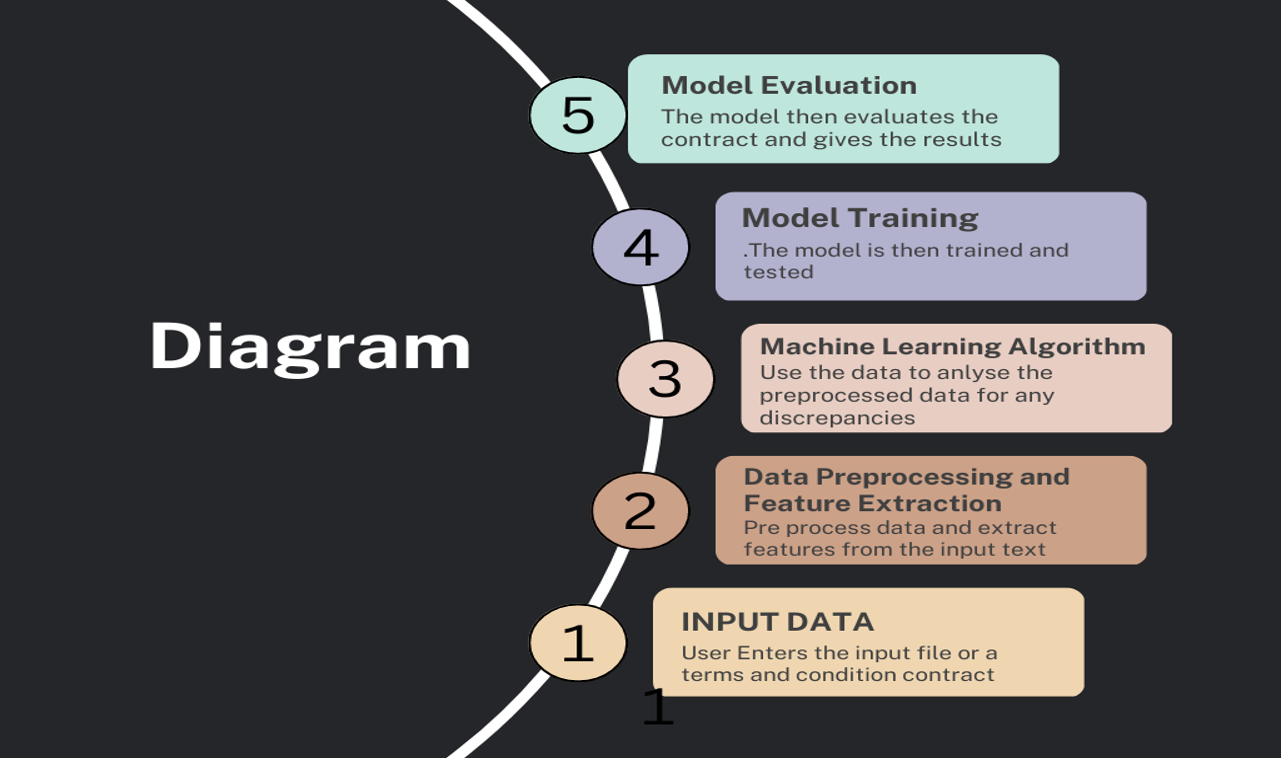
\includegraphics{Figures/Diagramoftheproposedsystem.png}}
\caption{\label{Figure::Diagram Of The Proposed System} Diagram Of The Proposed System  \ref{Figure::Diagram Of The Proposed System}}
\end{figure}





\newpage

\section{Mission Statement \label{Section::Mission Statement} }
The primary purpose of this project is to protect stakeholders from falling victim to deceptive clauses in contracts that may undermine their best interests, either intentionally or unintentionally or via other disruptive means. These clauses could cause harm to the signing party through various means, such as monetary loss or other negative consequences that may impact the livelihood of the concerned stakeholder as a whole. 
The proposed machine learning software system aims to detect and flag such fraudulent clauses in terms and conditions contracts, thus empowering stakeholders to make informed decisions before committing to an agreement. 
By leveraging advanced machine learning algorithms, the system will analyze and identify potential risks in the contract language. This approach ensures that stakeholders are aware of any hidden or obscure terms that could be detrimental to their interests. In addition to enhancing the transparency of contractual agreements upheld in a court of law, the software will enable users to negotiate better terms, minimize potential disputes, and ultimately establish a more secure and trustworthy contractual environment.
\chapter{Scope \\
%\small{\textit{-- Team-11}} 
\index{Chapter!Scope}
\index{Scope}
\label{Chapter::Scope}}



\section{Identification\label{Section::Project Identification} }


\section { Document Overview \label{Section::Document Overview} }



\section{System Overview\label{Section::System Overview}}
% The primary goal of this project is to develop a machine learning model that assists stakeholders in avoiding deception by clauses in terms and conditions (T\&C ) contracts. This approach will automatically analyze all clauses within the contract, providing stakeholders with the necessary information to decide whether to proceed or not.
% Several popular machine learning libraries, such as scikit-learn \cite{scikit-learn}, the Natural Language Toolkit (NLTK) \cite{nltk}, and Keras \cite{keras}, will be utilized to create the model. Flask \cite{flask} and Django \cite{django} will be employed to develop the web application, enabling users to upload T\&C contracts in text or PDF formats and evaluate the presence of any deceptive clauses. Scikit-learn, NLTK, and Keras are widely used libraries for machine learning tasks.
% We will start by selecting a dataset of T\&C contracts that have been identified as containing fraudulent or unclear clauses. The scikit-learn and Keras libraries will be used for feature extraction, where we can extract relevant information from the text. After extracting the features, we can use them to train a machine learning AI model using the scikit-learn engine.
% Once the AI model is trained, it can be evaluated using the Keras library to determine its accuracy. If the model performs well, it can be used to identify whether clauses in T\&C contracts are fraudulent or unclear.
% In summary, this project aims to create a machine learning model that helps stakeholders avoid deception in T\&C contracts by automatically analyzing the clauses within the contract. By using popular libraries and web development frameworks, the model will provide stakeholders with valuable insights and help them make informed decisions about whether to proceed with an agreement or not.

% \begin{figure}
% \centering
% \scalebox{0.53}{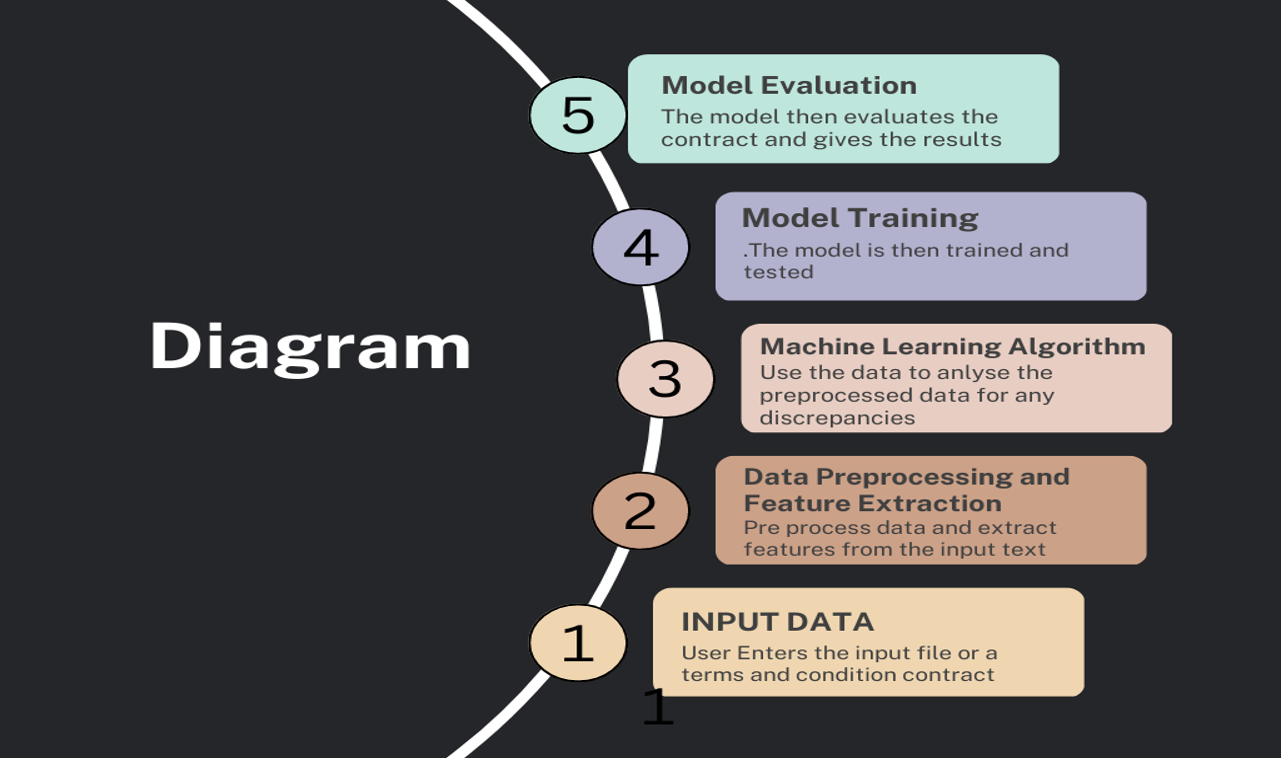
\includegraphics{Figures/Diagramoftheproposedsystem.png}}
% \caption{\label{Figure::Diagram Of The Proposed System} Diagram Of The Proposed System  \ref{Figure::Diagram Of The Proposed System}}
% \end{figure}

\chapter{Referenced Documents \\
%\small{\textit{-- Team-11}} 
\index{Chapter!References}
\index{References}
\label{Chapter::References}}

\begin{itemize}
    \item IEEE Std 1362-1998, IEEE Guide for Information Technology—System Definition—Concept of Operations (ConOps) Document, Approved March 19, 1998.

    \item Dr. Muresan, David Darian. Lecture-5, Lecture-05-Concept Of Operations( ConOps), Stevens Institute Of Technology, 2023
    \item Dr. Muresan, David Darian. Lecture-10, Lecture-10-Requirements Analysis, Stevens Institute Of Technology, 2023
    \item Dr. Muresan, David Darian. Lecture-2, Lecture-2-Stakeholders, Stevens Institute Of Technology, 2023
    \item Dr. Muresan, David Darian. Lecture-3, Lecture-3-Business Requirements, Stevens Institute Of Technology, 2023
    \item Dr. Muresan, David Darian. Lecture-4, Lecture-4-User Requirements, Stevens Institute Of Technology, 2023
    \item Dr. Muresan, David Darian. Lecture-6, Lecture-6- Requirements Elicitation, Stevens Institute Of Technology, 2023
    

    
\end{itemize}
\chapter{Current System Or Situation \\
%\small{\textit{-- Team-11}} 
\index{Chapter!Current System Or Situation }
\index{Scope}
\label{Chapter::Current System Or Situation}}
The motivation behind developing this system is that currently, stakeholders, which in this case would be common person, without much knowledge about the law, are required to manually read through terms and conditions contracts which can often be super long, time consuming and notoriously confusing due to the amount and complexity of the legal terms used, that are at the end of the day, accepted in a court of law, which would be unfamiliar to a common person thereby, risking themselves of inflicting harm in a shape that may result in financial, personal or mental distress. While the option to consult a lawyer exists, it is not always feasible due to their high costs and availability constraints.

In the absence of an effective tool to navigate this challenging problem, the need for a solution like ClauseGuard became apparent. This system is designed to safeguard stakeholders from potential pitfalls hidden in deceptive clauses. By providing a machine learning-based analysis of contracts, ClauseGuard offers a reliable, user-friendly, and cost-effective alternative to traditional methods of consulting a lawyer, fostering a safer and more transparent contract review process.  

\section{Background, objectives, and scope \label{Section::Background,objectives and scope} }
The current system exists to ensure that stakeholders, typically common individuals, are equipped to agree to the terms and conditions contracts set forth by the initiating party. This process, however, is often lengthy, complex, time-consuming, and challenging for the average person to fully understand the implications of the contract. While professional consultation is an option, the high costs associated with it often render it an unfeasible choice.

The mission of the proposed system, Clauseguard, is to ensure that stakeholders can effectively parse through the terms and conditions contract presented by the initiating party. The ultimate aim is to make stakeholders aware of any deceptive or harmful clauses in the contract, thereby safeguarding them from potential financial, personal, or other forms of harm.
 The scope of the proposed system extends to stakeholders from any background ranging from a common person to a lawyer, govermental agencies and mega corporations who may encounter contractual agreements. The objective is to provide support and enhance their understanding of the contracts they engage with, regardless of the complexity of the legal language involved. 



% The primary purpose of this project is to protect stakeholders from falling victim to deceptive clauses in contracts that may undermine their best interests, either intentionally or unintentionally or via other disruptive means. These clauses could cause harm to the signing party through various means, such as monetary loss or other negative consequences that may impact the livelihood of the concerned stakeholder as a whole. The proposed machine learning software system aims to detect and flag such fraudulent clauses in terms and conditions contracts, thus empowering stakeholders to make informed decisions before committing to an agreement.

% By leveraging advanced machine learning algorithms, the system will analyze and identify potential risks in the contract language. This approach ensures that stakeholders are aware of any hidden or obscure terms that could be detrimental to their interests. In addition to enhancing the transparency of contractual agreements upheld in a court of law, the software will enable users to negotiate better terms, minimize potential disputes, and ultimately establish a more secure and trustworthy contractual environment.

\section { Operational policies and constraints \label{Section::Operational Policies and constraints}}
There are a number of operational policies and constraints that are applied to the proposed system.
\subsection{Operational Policies}
An operational policy can be defined as a general statement of required behaviour. The operational policy of clauseguard is as follows: 
\begin{itemize}
    \item Data privacy is a major cause of concern for the proposed system. Sensitive and confidential information would be shared on an open internet website. As such, the system must ensure that no information is stored on any backend servers in the form of "cookies", "tokens" or any similar data logging services. The system should respect data privacy laws partaining to each individual country and follow guidelines as set forth by that particular country. 
    
    \item The system must explicitly ask stakeholders for their consent for analyzing the submitted documents before using the system. This consent would be devised by a team of professional experts and lawyers so as to not hold the parent organization of clauseguard of any legal ramifications. 

    \item The system must utilize a sophisticated machine learning algorithm that is retrained and updated at intervals of every two months. This ensures that the model stays current with the evolving nature of legal language in contracts, reflecting the latest laws and regulations. Additionally, cross-checking with historical legal data is done during these updates to maintain consistency and accuracy. Periodic reviews by legal experts complement the machine learning model, ensuring its recommendations remain accurate and legally sound.

    \item the system must provide clear explanations for any detected clauses in the Terms & Conditions contracts. These explanations are devised by the system based on the analysis of datasets comprising other legal documents of similar nature and scope. This ensures that users not only receive information about potential issues in the contracts they're reviewing, but also gain an understanding of why these clauses may be problematic.
\end{itemize}

\subsection{Operational Constraints}
An operational constraint is an externally imposed condition that must be observed. The operational constraint of clauseguard is as follows: 
\begin{itemize}
    \item The machine learning algrothim would require extreme amounts of processing power and computational resources, which, on failing to secure, would severely limit the number of contracts that can be analyzed. It can also lead to network wide crashes and instability. 
    \item The model depends on the accuracy of the dataset on which it is trained. Lack of available legal documents can induce severe challenge on the authenticity and accuracy of the model. Some countries do not disclose legal documents into the public domain, thereby severely limiting the use of this model in certain geographic locations. 
    \item The model must be online 24/7 365 days of the week. Lack of server resources can cause an availability constraint. 
    \item The model must comply with data regulations  and privacy laws around the world. This constraint cannot be guranteed across every country, as each country has extremely wide definations of data privacy laws, failing to adhere can cause a ban of this sytem in that particular country. 
    \item The model must handle contracts written in different terminologies and structures used across various different countries. For example, Japanese legal system requires legal documents to start from the right to left. Training the model on many different structures is a significant operational constraint. 
    \item The model must ensure the security of private and sensitive data. This is also a major operational constraint as unethical hacking can lead to significant data leaks. 
    
\end{itemize}

\section{Description of the current system or situation \label{Section::Description of the current system or situation}}
The current system is being built with the primary objective of developing a machine learning model to aid stakeholders in identifying potentially deceptive clauses in terms and conditions (T\&C) contracts. This system functions by automatically scrutinizing all clauses within the contract, thereby equipping stakeholders with crucial information needed to make an informed decision regarding their agreement to the terms.
The system uses several machine learning libraries such as scikit-learn, natural language toolkit(NLTK) and keras for the creation of the model. 

Scikit-learn is a machine learning library in Python that provides tools for data analysis and modeling. In this system, scikit-learn is primarily used for preprocessing the dataset and training the machine learning model. It provides utilities for common machine learning tasks such as feature extraction, text representation, and model evaluation. For instance, scikit-learn's text feature extraction utilities can convert the text data in T&C contracts into a format that can be input to the machine learning model.
Natural Language Toolkit (NLTK) is a library in Python that provides tools for working with human language data (text).  In this system, NLTK is primarily used for tokenization (i.e. breaking up of sentences into each indidual alphabet, white space, special character, symbol etc), stemming (A process to remove the suffix from words such as ing), and lemmatization (converting the word into its root form and reducing the superlative of the word into its equivalent comparative, for example: oldest will be old), which are crucial steps in preprocessing the text data.

Keras is a high-level neural networks API in Python.  
It is used to define and train any kind of deep learning model. In this system, Keras is used to define the machine learning model structure and train the model using the preprocessed dataset.

Flask and Django are web development frameworks in Python.  In this system, Flask and Django are used to build the web application that allows users to upload T&C contracts and get the results from the machine learning model. Flask can handle simpler and smaller loads, while Django can manage more complex and larger loads. The choice between them would depend on the requirements and scalability plans of the system. Flask would be used for the inital build of the system followed by django for a more advanced model. 

The system operates by facilitating users to upload a T&C contract via a web interface, developed using Flask or Django. The uploaded contract undergoes a preprocessing step, where it's transformed into a suitable format for the machine learning model using libraries such as scikit-learn and NLTK.

The preprocessed data is then fed into a machine learning model, constructed and trained using the Keras library. This model evaluates each clause in the contract, assigning a risk score that represents the likelihood of the clause being deceptive or unfair.

The output provided to the user includes highlighted sections of the contract that have been flagged as potentially deceptive, along with a percentage indicator that quantifies the overall risk associated with the contract. For each highlighted section, the system also provides an explanation, derived from the model's analysis, clarifying why the clause was flagged.

With this information, the user is empowered to make an informed decision about whether to sign the contract or not. 
The breakdown of the system is as follows: 
\begin{itemize}
    \item Operational Environment and its characteristics: The current environemtn invloves stakeholders using a web platform to upload their T\&C contract into a web interface. 
    \item Major system components and the interconnection among those components: The system comprieses of a machine learning model that is trained on a vast amount of datasets invlovling legal documents from various bracnches of the law such as crimaal law, corporate law, copyright protect, patent law, etc. The model parses each line in the contract, signals out protential harmful clauses that may seek to cause harm to the signing party in the shape of montery or mental duress, and quantifies the risk carried with the contract signified by a percentage. Furthermore, the model genewrates expplainations for the harmful clauses it has highlighted. 
    \item Interfaces to external systems or procedures: The system can be accessed on any platform, device and operating systems. Similar to chatgpt, an api for the model will be released whcih can be integrated into propirety systems that are otherwise not avaialbe to the general public and are the intellectual property of their respective owenrs. 
    \item Capabilities, functions, and features of the current system: The system's objective is to analayze and interpret complicated legal terms, identifying potentially harmful clauses and providing layman explainations to the user. The system's function includes parsing throug each line of the document, running the parsed text through the machine learning model and generating a small report accessable within the website itself that includes a risk assessment percentage as well as a succint explaination, 
    \item e)                \begin{figure}[H]
    \centering
    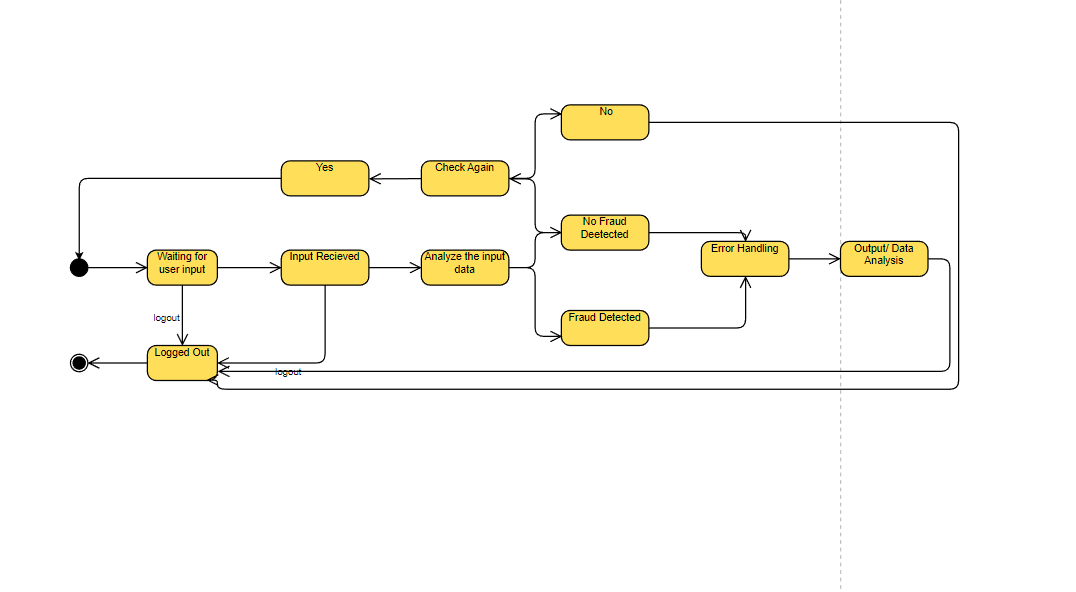
\includegraphics[scale=0.83]{Figures/state machine.png}
    \caption{State Machine View of the diagram \ref{fig:state machine}}
    \label{fig:state machine}
\end{figure}
   

    \item Cost of system operations: The cost of running the system would depend upon the amount of resources that it would take to run the model on servers accessible throughout the world wide web whist analyzing millions of documents concurrently. Load balancers and other such infrastructure must be set up to ensure the working for the model. Infrastructure like the Amazon AWS could be used to set up the model. This would solve the problem with data protection too.  Maintenance would require additional funds. Overall, a cost in the 7 figure range is expected for the initial version of the system 

    \item Operational risk factors: Several operation risk factors could occur which include inaccurate intepretation and explaination, legal reprucssions, confidential Data leaks, Security breaches, server crashes, instability, low accuracy, inaccurate percentages and so on. 
    \item Performance characteristics: The model should be fast, accurate and able to process large quantities of data. To ensure these non-functioanl requirements, the model can be set up on additional infrasture such as could bases services. Amazon AWS would benefit the model tremedously. 
    \item Quality attributes: The model should aim for high availability, reliability and secuity. Becuase of the nature of deleaing with legality of a country, accuracy, avaialbity and reliability are of utomost importance. 
    \item Provisions for safety, security: Due to the nature of the model itself, sensitive and confidential data will be shared. The model must ensure data privacy and secuity of the system to prevent potential breaches and subsequent leaks of confidential data. The system must be designed to ensure high frequency of backed up data to guarantee swift recovery of said data if  operational failures occur. 
\end{itemize}

 



\section{Modes of operation for the current system or situation \label{Section::Modes of Operation for the current system or situation}}
The system will operate on various modes of operation throughout its lifecycle as detailed below: 
\begin{itemize}
    \item Training Mode: This mode is only accessible to the system's developers and not to the end users. It plays a crucial role in the functioning of the system as this is where new features are developed, the model is trained on additional datasets, and existing defects are patched. The training mode uses large amounts of T\&C contracts to train the machine learning model to understand the structure, language, and meaning of various clauses. This process allows the model to learn how to distinguish between benign and deceptive clauses. Enhancements and updates to the system are made in this mode before being deployed to the Operational Mode. 
    \item Operational Mode: This model is the primary end product of the system used by the users to upload T\&C contracts for analysis. The system would use the model developed in the training mode to evaluate the uploaded contract. It identifies potentially deceptive clauses, calculates the overall risk associated with the contract, and provides explanations for flagged sections. The results are then displayed to the user, who can use this information to make an informed decision about whether to sign the contract.
    \item Emergency Mode: This mode serves as a contingency plan, activated in the event that both the Primary and Training modes experience operational failures. The Emergency Mode relies on a legacy version of the currently deployed primary model. This fallback mechanism ensures continuity of service even in the face of unforeseen disruptions. While it may not have the most recent updates and features available in the Primary Mode, the Emergency Mode is designed to effectively analyze T&C contracts and identify deceptive clauses, thereby maintaining the core functionality of the system. Regular checks and minor updates are carried out to ensure that the Emergency Mode is always ready for activation, should the need arise. This robust backup plan contributes to the system's resilience and reliability, offering users a dependable tool for contract analysis at all times.
    


\end{itemize}


\section{User classes and other involved personnel \label{Section::User Classes and other involved personnel}}
Clauseguard would involve the participation several user classes and  personal either directly or indirectly depending upon their interaction with the system as given below: 
\begin{itemize}
    \item End User: The end users are the primary users of clauseguard. They interact directly with the system by uploading the T\&C contracts for analysis. Their interaction is via the web platform, with the aim of identifying deceptive contracts in T\&C contracts. They don't require any skill levels except basic computer skills. 
    \item Developers: They are the primary coders of the system. Their responsibilities include, implementing new features, functionality and maintenance of the system. They require high skill levels in the fields of programming and problem-solving as they require a high level of technical skill and familiarity with the underlying technology.
    \item Machine Learning Specialists: ML specialists work to continually improve clauseguard's machine learning algorithm. They are responsible for training the model on new datasets, testing performance and implementing updates as needed. Their interaction is through machine learning libraries used in the development of the model. 
    \item CyberSecurity Experts: These individuals play a crucial role in safeguarding the ClauseGuard system from unauthorized access and potential security threats and are arguably the most important stakeholders in the functioning of clauseguard as a service. They are tasked with the responsibility of thwarting attempts by unethical entities, often referred to as hackers, who might attempt to breach the system and gain access to confidential data. Cybersecurity experts work diligently to identify and secure any potential vulnerabilities in the system that could be exploited for malicious purposes. Their interaction with the system spans across all areas, but they primarily focus on the system's edge cases and potential weak points that could be susceptible to breaches. They are proficient in the latest cybersecurity protocols and techniques and utilize this expertise to constantly enhance the system's security measures. In addition, they collaborate closely with the system administrators and developers to ensure that security is integrated into all aspects of the ClauseGuard system, from the web application to the machine learning model itself. Their work helps maintain the trust of the end-users by ensuring that their interactions with the system remain secure and confidential.
    \item Legal Consultants: Although their involvement may not be direct, they nevertheless, play a crucial role in the development of the model. They review the machine learning model's output to ensure its accuracy and make recommendations for improvement based on their legal expertise. They interact indirectly with the system by providing feedback and suggestions for model enhancements based on their understanding of legal terminologies and concepts.
    \item Commercial enterprises stand to gain significantly from the use of the ClauseGuard system. These entities often engage in complex transactions that involve extensive legal contracts. With the help of ClauseGuard, they can quickly and efficiently review these contracts, expediting the deal-making process. For instance,  the  purchase of Activision-Blizzard by Microsoft made headlines across the tech industry. In such scenarios, missing or overlooking crucial legal details can lead to considerable impediments, potentially blocking the deal altogether which happened in the case of Microsoft acquiring Activision-Blizzard. ClauseGuard can mitigate such risks by identifying potentially harmful or unclear clauses that could jeopardize the agreement. This can save enterprises substantial time and resources, while also providing them with a layer of protection against contractual pitfalls. Similar to end users, commercial enterprises need only basic computing skills to access clauseguard. 

\end{itemize}


\section{Support environment \label{Section::Support Environment}}
Clauseguard will have a number of support systems in place that will fortify the absolute working of the system to its fullest capacity. 
\begin{itemize}
    \item Clauseguard will have a dedicated technical support team. This team will handle technical queries, troubleshoot reported issues and work on continuous improvement of the system. 
    \item Since clauseguard would primarily be virtual, the equipment and facilities would involve robust server architecture preferbly on cloud bases services such as AWS, load balancers for handling multiple connection requests and IT infrastructure for the support team to handle issues effectively. 
    \item Clauseguard would have a customer service team and infrastructure to manage user inquiries, issues and feedbacks. This platform would involve efficient tracking and resolution of support tickets. 
    \item ClauseGuard , being a cloud-based application, would use secure cloud storage services to store user data and application elements essential for the functioning of the system. It is to be noted that any personal or confidential data will not be stored in any capacity. 
\end{itemize}





\chapter{Justification for and nature of changes \\
%\small{\textit{-- Team-11}} 
\index{Chapter!Justification for and nature of changes }
\index{Justification for and nature of changes}
\label{Chapter::Justification for and nature of changes}}\



\section{Justification of changes  \label{Section::Justification of changes} }
Justification for the changes of the proposed systems is outlined below: 
\begin{itemize}
    \item New or modified aspects: The rapidly changing legal landscape and increasing complexity and ambuity in T\&C contracts propelled the need for an efficent and reliable system that can adapt and and update itself based on the latest laws and guidelines. 
    \item Limitations of the current systems: At the moment, most contracts are manually reviewed by legal professionsals. This process is time0consuming, tedious and prone to error. Furthermore, the interpretation of different terms and conditions may vary between different individuals leading to inconsistancies in evaluations. 

    \subsection{Justification for a new or modified system}
    Clauseguard can effectively counter the challenges faced by the current system as outlined below: 
    \begin{itemize}
        \item With the advent of the COVID-19 pandemic, there has been a significant uptick in the usage of digital contracts. This transition has led to a surge in data volumes that traditional methods of review cannot efficiently handle. ClauseGuard's machine learning model, with its inherent ability to process and analyze vast amounts of data swiftly and accurately, stands to offer an invaluable service in this context. It can help stakeholders navigate through the labyrinth of digital contracts, ensuring they are informed and protected. This capability is not just a convenience; it is a necessity in the rapidly digitizing world, where the velocity and volume of contractual agreements are ever-increasing. 
        \item The machine learning system aims to automate the evaluation of contracts, significantly reducing the time and resources required, thereby leading to lower operational costs. It can also improve consistency in evaluations by reducing subjective human interpretation.
        \item The capability to autonomously detect deceptive or unclear clauses within contracts has become increasingly necessary in today's rapidly evolving legal landscape. Contracts are becoming more intricate and are subject to frequent revisions due to changing regulations and business practices. These complexities often make it challenging for individuals to fully comprehend the terms, leading to potential misinterpretations and unintended commitments. An automated system that can reliably dissect and interpret these complexities not only promotes transparency but also serves as a protective measure for stakeholders. 
    \end{itemize}
    
\end{itemize}


\section{Description of desired changes \label{Section::Description of desired changes}}
Clauseguard has a number of capabilites, interfaces and personel changes which are highlighted below: 

\begin{itemize}
    \item Capability Changes: The implementation of the machine learning model will introduce new capabilities such as automated analysis of T&C contracts, detection of deceptive or unclear clauses, and explanations for detected clauses. While the original system relied on manual inspection and comprehension of contract clauses, the new system will automate this process, significantly reducing the time and effort required to review contracts. Moreover, it would be cost effective for those individuals who otherwise, would not abe able to affort professional legal opinion.
    \item System Processing Changes: The machine learning model process the uploaded contracts, analyze the clauses, and output results indicating the presence of any deceptive clauses along with explanations for the same. 
    \item  Interface Changes: The user interface will be modified to allow users to upload contracts and view results. This interface will need to be intuitive and user-friendly, providing clear instructions on how to upload contracts and view results. Changes to the interface will also need to accommodate the presentation of results, which will now include highlighted clauses and their explanations.
    \item Personnel Changes: The development and maintenance of the machine learning model will require personnel with expertise in machine learning, natural language processing, and contract law. Additionally, user training may be required to educate users on how to interact with the new system and interpret its outputs.
    \item Personnel Changes: The development and maintenance of the machine learning model will require personnel with expertise in machine learning, natural language processing, and contract law. Additionally, user training may be required to educate users on how to interact with the new system and interpret its outputs.
    \item Environment Changes: The implementation of the machine learning model will digitize the contract review process, requiring an operational environment that can support the deployment and use of this technology. This may involve changes to existing IT infrastructure and the adoption of new technologies to support the model.
    \item Operational Changes: The introduction of the machine learning model will fundamentally change how contracts are reviewed traditionally. Instead of manually reading through contracts, users will upload them to the system for analysis. This will change the operational procedures and daily work routines of the users.
    \item Support Changes: The implementation of the machine learning model will necessitate changes in the support requirements. Technical support will need to be available to address any issues that arise with the use of the machine learning model. Moreover, regular updates and maintenance will be required to ensure the model remains up-to-date with changes in contract law.
    \item Other Changes: As a result of the implementation of the machine learning model, there may be changes to the time required to review contracts. As the process becomes more automated, it is likely that contract review times will be significantly reduced, allowing for quicker decision-making, faster legal processes and reduction in the cost of paralegal teams. 














\end{itemize}


\section{Priorities among changes \label{Section::Priorities among changes}}
The proorites for the system ClauseGuard are highlighted below: 
\begin{itemize}
    \item Essential Features: \begin{itemize}
        \item The core feature of the system is its ability to identify and highlight potentially fraudulent clauses within a contract. Without this feature, the system would not serve its primary purpose. Failure to implement this would lead to users not being able to identify potential risks in contracts.
        \item The system should be able to assign a risk percentage to each contract, indicating the level of potential fraud. This is vital as it quantifies the risk involved, aiding users in their decision-making process.


        \item Each identified risk should come with an explanation to help users understand the reasons why the clause has been flagged as fraudulent. Without this feature, users may be left confused about the nature of the risk involved.


       
        




    \end{itemize} 

    \item Desirable Features: 
    \begin{itemize}
        \item While not essential, having an intuitive and easy-to-use interface would greatly enhance user experience, encouraging more frequent use and increasing user satisfaction.

        \item The ability to integrate with common document management systems would make the application more versatile and convenient to use. It would allow users to directly upload contracts for analysis from a wide range of document format systems.

        \item  An ability to analyze and present a comparison of risk percentages. This feature would provide users with an onjective metric along with an explaination of why that specific clause was highlighted intended to allow the user to make an informed decision. The decision, ultimately, is left upto the descretion of the user. 

    \end{itemize}

    \item Optional Features: 
    \begin{itemize}
        \item The ability to process and analyze contracts in multiple languages would increase the usability of the system across different geographic locations and allow for greater control over the scanned documents.
        \item A feature that allows multiple users to view and discuss the same contract in real-time. This can facilitate faster decision-making, especially in larger teams similar to that of what the platform "Overleaf" does for LaTeX documents.
        \item Providing API access would allow third-party developers to integrate ClauseGuard's features into their own applications.
        \item Allowing users to directly sign off on safe contracts via popular e-signature platforms could streamline the contract approval process such as adobe signature. 
        \item A feature that allows users to customize the risk percentage threshold that triggers a flag, enabling a more personalized user experience.
        \item  feature that tracks and displays changes made to a contract over time, helping users see how the risk assessment has evolved.

    \end{itemize}

\end{itemize}




\section{Changes considered but not included \label{Section::Changes considered but not included}}
Some features that were considered for ClauseGuard but were not included as follows: 
\begin{itemize}
    \item A Real-Time Fraud Detection feature would have allowed the system to analyze contracts and detect fraudulent clauses as the user is typing or editing the contract. However, due to the significant computational resources required for real-time analysis and the potential disruption to the user experience due to lag or delay, this feature was not included.
    \item A feature for automatic contract modification which would allow the system to suggest modifications to contracts to eliminate or mitigate the risk of identified fraudulent clauses. However, this was not included due to the potential legal implications and the complexity of accurately generating legally sound contract language.
    \item An AI chatbot feature was considered to provide immediate assistance to users. However, due to the complexity of developing a chatbot that can accurately understand and respond to a wide range of user queries, this feature was not included.




\end{itemize}
Note: Although the above features are not included at this time of development, these are features that could be looked at to add on at a later stage of ClauseGuard's life cycle. 

\section{ Assumptions and Constraints \label{Section::Assumptions and Constraints}}
The assumtions and constraints of clauseguard are as follows:
\begin{itemize}
    \item Assumptions: An assumption is defined as a condition that is taken to be true. Some of the assumptions for ClauseGuard are: 
    \begin{itemize}
        \item Data Availability: We assume that the system will have access to a sufficient number of sample contracts with and without fraudulent clauses for training the machine learning model.
        \item User Literacy: We assume that users have a basic understanding of contractual language and terms, as this will influence how they interact with the system and interpret the risk assessments.
        \item Scalability: We assume that the number of contracts to be analyzed will increase over time as more users adopt the system, necessitating a scalable architecture.
        \item Legal Compliance: We assume that all analyzed contracts will be in compliance with local laws and regulations, which the system will need to be updated to reflect.






    \end{itemize}
    \item Constraints: A constraint can be defined as an externally imposed limitation placed on the new or modified system or the processes used to develop
or modify the system. Some of the constraints of ClauseGuard are as follows: 
\begin{itemize}
    \item Budgetary Constraints: The development and maintenance of the system is subject to the availability of funds. This might limit the number of features that can be implemented at a given time.
    \item Time Constraints: The system must be developed and made operational within a specified timeframe. This could limit the amount of testing and refinement that can be done before launch.
    \item Privacy Constraints: The system must comply with data privacy laws and regulations, such as GDPR. This could limit the type of data that can be collected and how it can be used. The system must also take into account some countires that are cut off from the rest of the world such as Russia, Azerbaijan, Kyrgyzstan etc. 


\end{itemize}
\end{itemize}


\chapter{Concepts for the proposed system \\
%\small{\textit{-- Team-11}} 
\index{Chapter!Concepts for the proposed systems }
\index{Concepts for the proposed system}
\label{Chapter::Concepts for the proposed system}}\



\section{Background, objectives, and scope \label{Section::Background,objectives,and scope proposed}}
The rationale for the proposed approach is that it can be challenging for people to spot fraudulent elements in contracts since they are sometimes buried within lengthy and complicated terms and conditions. The suggested system's goal is to identify dishonest clauses in contracts using machine learning techniques, which will increase the contracts' fairness and transparency for all parties. The proposed system's scope includes contract analysis across a range of industries, including technology, insurance, and financial services.


\section{Operational policies and constraints \label{Section::Operational Policies and Constraints proposed}}
The system must make sure that user data is not abused or disclosed without permission, and that the data it gathers and analyzes is handled securely and confidentially.
The system must be precise and trustworthy in spotting contract fraud. The algorithms and outcomes of the system must be rigorously tested and validated for this.


\section{Description of the proposed system \label{Section::Description of the proposed System proposed}}
To find potentially dishonest clauses in contracts, the suggested method will employ machine learning algorithms and natural language processing. Contracts will be analyzed by the system, and any clauses that seem to be unfair, misleading, or deceptive will be flagged. The system will also explain its findings so that consumers may comprehend the justification for the system's choices.



\section{Modes of operation \label{Section::Modes of operation proposed}}

The suggested system will function in two different ways:

In manual mode, a user can upload a contract to the system for analysis, and the system will then give that analysis.

Real-time mode, when the system continuously checks contracts for dishonest clauses and alerts the user to any potential problems.


\section{User classes and other involved personnel \label{Section::User Classes and other involved personnel proposed}}
People and organizations involved in contract formulation and approval will make use of the suggested system. These professionals working with contracts include attorneys, contract managers, compliance officers, and others. Additionally, the system will work with specialists in machine learning who will be in charge of enhancing and refining the system's algorithms.


\section{Support environment \label{Section::Support Environment proposed}}
User guides, online help, and a customer service team will all be part of the support system for the planned system. The system will also include a feedback tool that will let users comment on how well the system is working and recommend changes. To guarantee that the system is operating at its peak performance, routine upgrades and maintenance will be offered.



\chapter{Operational scenarios 
%\small{\textit{-- Team-11}} 
\index{Chapter!Operational scenarios }
\index{Operational scenarios}
\label{Chapter::Operational scenarios}}\

A scenario can be defined as a  step-by-step description of how the proposed system should operate and interact with its users and its
external interfaces under a given set of circumstances. The operational scenario for the following proposed system is outlined below
\begin{itemize}
    \item Normal Operation Scenario: The user navigates to the website, facilitated by a user-friendly interface designed for ease of use. They are greeted by clear instructions and prompts guiding them to upload a Terms and Conditions (T\&C) contract. This can be in various formats such as text, PDF, or LaTeX document, providing ample flexibility to the user.

Once the contract is uploaded, the system initiates the preprocessing stage. This involves cleaning and formatting the text data, utilizing Natural Language Processing techniques such as tokenization, stemming, and lemmatization. This step ensures that the machine learning model receives the data in a suitable format for analysis.

Upon completion of the preprocessing stage, the data is fed into the machine learning model, which has been trained on a vast dataset of T\&C contracts. The model thoroughly scrutinizes the clauses in the contract, identifying any potential deceptive or unclear clauses.

The user then receives a comprehensive report, detailing the analysis results. The report includes a percentage counter indicating the proportion of potentially deceptive clauses found in the contract. Each flagged clause is highlighted, and clicking on it provides a brief explanation as to why it was flagged by the model.

With this detailed insight, the user is better equipped to make an informed decision on whether to proceed with the contract. To proceed with the contract, is left upto the discretion of the user. 

\item Stress handling scenario: A stress handling scenario occurs in a situation where multiple users simultaneously access the website, potentially leading to the analysis of millions of documents concurrently. In such high-demand situations, the system is designed to maintain operational efficiency, ensuring that all users receive a timely and accurate analysis of their contracts.

To manage this high traffic, the system utilizes a sophisticated load balancing mechanism. This mechanism dynamically allocates system resources to different tasks based on demand, ensuring that no single task is overburdened. The load balancer distributes the workload across various system servers located on strategic geographic locations, preventing any bottlenecks or system slowdowns.

Furthermore, the system is built with scalability in mind. It has the capacity to ramp up resources when demand surges, such as during peak usage hours. This ensures that even in times of heavy load, the system remains responsive and continues to deliver results promptly.

Lastly, the system employs robust error handling techniques. In the rare event of a failure or error, the system is designed to recover gracefully, minimizing the impact on the user. Alerts are sent to the system administrators to ensure rapid response and resolution.

Through these measures, the system can effectively manage stress scenarios, providing reliable, efficient service to all users, even during periods of peak demand.

    \item Error handling Scenario: An error handling scenario comes into play when a user attempts to upload a contract in an unsupported file format. In such a situation, the system is designed to promptly identify the issue and respond appropriately and in a timely manner.

Upon detecting an unsupported file format, the system triggers an error message. The system informs the user that the uploaded contract file format isn't supported and kindly prompts them to upload the contract again in a compatible format.

In addition, this error message includes a list of the supported file formats for the user's convenience. This  approach not only resolves the issue at hand but also educates the user about the correct file formats, preventing the same error from reoccurring in the future.

Furthermore, the system logs this error in a database. These logs are periodically reviewed by the system administrators to identify patterns and potential areas for system improvement. For instance, if a particular unsupported file format is frequently attempted by users, the team may consider adding support for that format in future system updates.

Thus the error handling scenario is designed to be user-centric in its approach and its commitment to provide a seamless, intuitive user experience. 

 \item Degraded Operation Scenario: A system degradation scenario comes into play when there's an unforeseen failure with the primary system. In such instances, our robust backup strategy ensures that service continuity is maintained, albeit the service may not be as robust as the primary model.

Upon detection of a primary system failure, the system automatically transitions to a legacy version. This redundancy plan allows users to continue accessing the system and uploading contracts for analysis, ensuring that the primary functionality of the system. remains available. This would also ensure that there is no monetary loss to the organization in the event of a catastrophic system failure. 

However, its important to note that while the legacy system is fully functional, it might not match the performance, accuracy, or feature set of the primary system. As it is an older version, it may process contracts more slowly, and its clause analysis might not reflect the most recent legal developments or algorithmic improvements.

During this degraded mode operation, users will be informed about the temporary switch to the legacy system via a notification on the website. This message reassures them that services are still operational, but also sets appropriate expectations about the temporary limitations they might experience.

Meanwhile, our dedicated team of technicians would be alerted to the issue and would begin troubleshooting the primary system. The goal would be to restore the primary system to full functionality as quickly as possible to minimize the time users spend operating under the degraded mode.

This degradation scenario works towards highlighting our commitment to service reliability and continuity. We understand that our users depend on our system, and we have contingency plans in place to ensure that unexpected issues don't interrupt the availability of our services.

    \item Emergency scenario: In the event of a security breach, our system swiftly transitions to a minimally functioning mode to prioritize data protection and system integrity.

Upon detecting a potential security threat, our system automatically triggers its emergency protocol. This protocol includes limiting user access, suspending non-essential operations, and activating enhanced security measures. The aim is to isolate the breach, protect sensitive data, and prevent further unauthorized access to ensure no confidential or sensitive data is leaked.

During this emergency mode, users may encounter restricted functionality. Access to majority of the services might be temporarily suspended , and the overall system performance may be reduced. However, these measures are critical to maintaining the security of the system and safeguarding user's data.

Simultaneously, our cybersecurity team would be alerted to the situation. These experts would immediately initiate an investigation into the breach, working tirelessly to neutralize the threat and restore the system to full functionality. Users would be notified about the situation and would be kept informed about progress towards resolution.

This emergency scenario highlights our commitment to data security and system integrity. We understand the critical importance of protecting sensitive information, and our system is designed to respond effectively to any security threats, minimizing potential damage and disruption.

    \item Backup Scenario: In circumstances where data integrity is compromised, due to a security breach, system error, or data corruption, or unethical stakeholders trying to  gain access, the system would resort to its backup protocols to ensure data preservation and service continuity.

Our system routinely creates secure backups of all operational data. These backups are securely encrypted and stored off-site to ensure data safety. The frequency of these backups is decided based on the criticality and volume of the data, ensuring minimal data loss in case of unexpected events.

Upon the detection of any data corruption or loss, the system triggers its backup recovery procedure. The most recent unaltered backup is identified, and the data is seamlessly restored to the system. During this process, the system may operate in a limited capacity to ensure the stability and accuracy of the data restoration process.

Meanwhile, our dedicated teams would work on identifying and rectifying the cause of the data loss or corruption, making sure the same issue does not recur. Users are kept informed of the situation and provided with any necessary guidelines or precautions to ensure their data safety.

This backup scenario is an integral part of our commitment to providing a reliable and secure service.
    \item Maintenance Scenario: In the interest of continuous improvement and to ensure optimal performance, the system is periodically placed into a maintenance mode. During these scheduled maintenance periods, updates are performed, enhancements are made, bugs are addressed, and routine checks are conducted to ensure the overall health and security of the system.

These maintenance events are carefully planned and scheduled during periods of expected low usage to minimize inconvenience for our users. Advance notifications are sent to users to inform them about the maintenance schedule and the expected duration of downtime. The importance of the service is understood and the every effort is being made to keep these periods as brief as possible.

During maintenance, the system might be temporarily unavailable or operate with limited functionality. However, these periods are crucial for implementing system upgrades, installing security patches, and performing hardware checks, all aimed at providing a seamless, secure, and efficient service.

Upon completion of maintenance, the system returns to its normal operational state. Users are promptly notified that they can resume using the service as usual. Our dedicated support team remains available to address any queries or concerns users may have post-maintenance.

This maintenance scenario is vital to maintaining the high standards of our system, safeguarding data, and offering an enhanced user experience. It reflects our commitment to delivering a reliable, secure, and up-to-date service to all our users.
\end{itemize}



\chapter{Summary of impacts \\
%\small{\textit{-- Team-11}} 
\index{Chapter!Summary of impacts }
\index{Summary of impacts}
\label{Chapter::Summary of impacts}}\
The proposed system "clauseguard" will have significant operational impacts on users, developers, and the support and maintenance organizations. 
For users, particularly legal and paralegal teams, the system seeks to induce change into the fundamentals of the existing workflow. Instead of manually reviewing contracts, users will now have the ability to upload them to the system and then analyze the generated reports to identify potentially fraudulent activities along with the explanations. This is expected to reduce the time spent on contract reviews, thereby increasing productivity and allowing more focus on complex cases that require human intervention.

Developers will face a shift in their roles as they will have to maintain and update the machine learning model regularly. This includes ensuring that the model is trained on up-to-date data, optimizing it for better performance, and resolving any issues that might arise.
Support and maintenance organizations will  need to familiarize themselves with the working of the ClauseGuard system. They will have to handle new kinds of queries and issues that may arise from the system's operation. The organizations will also have to develop a robust data backup and recovery system to protect the data fed into ClauseGuard.
It is to be noted that although these impacts are anticipated or expected, they might change over time during the actual implementation of the system.







\section{Operational impacts\label{Section::Operational Impacts}}
Operational impacts can be defined as how the system would evolve to become part of the new operational environment. The operational impacts are highlighted below: 
\begin{itemize}
    \item Since the model is platform independent, interfaces with primary or alternate computing platforms are not required except in the case of data recovery programs. 
    \item The procedure for reviewing contracts will change, as the model will be able to flag potentially deceptive clauses, speeding up the review process and reducing the burden on legal personnel.

    \item The model will require a database of contracts and legal clauses to function optimally. This data may be obtained from existing contract databases, open source legal databases, and other relevant sources.

    \item The system will now require digital versions of contracts to be input for analysis, which may increase the volume of data being handled. 
    \item Due to the need to train and improve the model, there may be changes in data retention policies, especially for contracts and related legal documents.

    \item Investment will be required for the development, implementation, and maintenance of the system, as well as additional cloud infrastructure required to effectively scale the system and ensure maximum availability to the tune of 99.999%  .
    \item While the system is expected to reduce the risk of entering into contracts with deceptive clauses, there may be new risks associated with data security and system reliability as well as the accuracy as existing laws are changed to support the ever evolving landscape of the legal world. 






\end{itemize}




\section{Organizational impacts \label{Section::Organizational Impacts}}
Organizational impact can be defined as the impact on the stakeholders of the system. The impact can be direct or indirect, positive or negative. The breakdown of organizational impact is given below: 
\begin{itemize}
    \item Legal personnel will need to review flagged clauses, in order to improve the accuracy of the model as their input determines the effective working of the model. 
    \item It personnel will have responsibilities for maintaining the system. 
    \item Positions related to manual contract review may be reduced, while positions related to system support and maintenance may increase as well as cloud infrastructure specialists and DevOps engineers. 
    \item Existing personnel will need to be trained to use the system and understand its outputs.

    \item There may be increased demand for personnel with skills in machine learning and contract law. Some personnel may need to be relocated to roles where these skills are more needed and where the model is being actively developed. 
    \item In case of an emergency or disaster that disrupts normal operations, contingency plans will need to be put in place. This will require a subset of personnel who are trained in operating the system to be available to set up and manage operations at an alternate site.

The number of personnel required will depend on the complexity of the system and the volume of contracts that need to be reviewed during the contingency operation. Given the technical nature of the system, these personnel should have a good understanding of machine learning principles, the specific model used, and the legal knowledge necessary to interpret the system's output.

Having a well-trained, technically competent contingency team will ensure that contract review can continue with minimal disruption, even under less than ideal circumstances. This is particularly important given the potential legal and financial implications of contracts with deceptive terms and conditions.




\end{itemize}




\section{Impacts during development\label{Section::Impacts During Development}} 
The impact of the system ClauseGuard during development is as follows detailed below: 
\begin{itemize}
    \item Users, developers, legal consultants, and support personnel will need to be involved in discussions and studies to define system requirements and objectives. The aforementioned stakeholders must be in consensus for the effective development of the system. Induced constraints by the way of conflicting requirements should be avoided at all costs to mitigate the risk of stalled development. 
    
    \item Users and support personnel will need to be involved in reviews and demonstrations of the system, to ensure it meets the organization's needs. They should receive additional training to ensure the maximum efficiency of the system. 

    \item During development, the new system may need to be run in parallel with existing procedures to ensure no disruption to contract review processes.



    \item System testing may require additional resources and may impact normal operations, as potential bugs and issues are identified and fixed.







\end{itemize}







\chapter{Analysis of the proposed system \\
%\small{\textit{-- Team-11}} 
\index{Chapter!Analysis of the proposed system }
\index{Analysis of the proposed system}
\label{Chapter::Analysis of the proposed system}}\

The system "Clauseguard" provides several benefits which are highlighted below: 
\begin{itemize}
    \item The "ClauseGuard" system mundanes access to legal advice, bringing complex knowledge of terms and conditions contracts to the fingertips of the everyday user. By leveraging advanced machine learning algorithms, it empowers individuals and organizations with the ability to identify potentially fraudulent clauses without the need for extensive legal consultation.

" 
    \item By automating the examination process, "ClauseGuard" drastically reduces the margin of human error that may occur even with the involvement of experienced legal consultants. The model's capacity to scan vast amounts of data ensures a thorough, comprehensive review of contractual content, which traditionally could take considerable time and resources.
    \item The system is designed with user-friendliness at its core, making it accessible to any stakeholder with basic computational skills. This opens up the domain of legal understanding, traditionally seen as complex and out of reach for many, to a broader audience. It democratizes the process of understanding and evaluating legal contracts, thereby helping users make more informed decisions.
    \item "ClauseGuard" not only brings about significant cost savings but also enhances the speed and efficiency of contract reviews. It can be utilized by small businesses, corporations, and individual users, thereby promoting a culture of transparency and fairness in contractual agreements.
    \item The system's flexibility allows it to adapt to varying legal environments and contract structures. This means that as legal language and contract formats evolve, "ClauseGuard" can be updated and trained to understand these changes, ensuring it remains a valuable tool for contract review.

    \subsection{Limitations}
    Despite the advantages clauseguard brings to the everyday world, it also has certain limitations which are highlighted below: \begin{itemize}
        \item The performance of the model is contingent on the quality of the data it's trained on. Poor quality data can result in inaccurate detections.
        \item As legal language and fraud strategies evolve, the model will need continuous updates and training to maintain its effectiveness.
        \item As clauseguard is being deployed on an international scale, this presents with a unique set of challenges. Given the varying legal definitions and structures across different countries, the system must be equipped to incorporate a vast array of terminologies and documents. The complexity of the task is amplified by the intricate and distinctive nuances of legal language in different jurisdictions. The system's ability to effectively interpret and adapt to these differences is crucial in its functionality and effectiveness.


        \item  "ClauseGuard" must not only recognize nuances but also articulate them to the user in a comprehensible manner. Translating complex legal jargon into user-friendly language is no simple task, particularly when considering the diverse and intricate nature of legal contracts. This translation process, however, is essential to meet the system's goal of making legal knowledge accessible to the common man.
        \item It is also extremely important to note the potential ethical implications of an automated system providing legal advice. While clauseguard is designed to identify potentially deceptive clauses, it's not a replacement for professional legal advice. The model must be clear in communicating its role as a supportive tool rather than a definitive legal authority.
        




        
    \end{itemize}

\subsection{Advantages}
        Clauseguard provides several key advantages. 
        \begin{itemize}
            \item The system can easily scale to handle larger volumes of contracts without a proportional increase in resources or time.
            \item Unlike human reviewers, "ClauseGuard" offers consistent performance, unaffected by factors like fatigue or bias.


        \end{itemize}
        \subsection{Disadvantages}
        Clauseguard has some disadvantages. 
        \begin{itemize}
            \item Potential for False Positives/Negatives: The model may occasionally flag non-fraudulent clauses as fraudulent (false positives) or miss fraudulent clauses (false negatives).
            \item There can be significant initial costs associated with setting up the system and training the model.
            \item The efficiency of ClauseGuard is directly proportional to the quality of data it receives. If the input data is poorly written or ambiguous, the model's ability to accurately detect deceptive clauses could be compromised.

            \item  While machine learning models can analyze and draw conclusions from vast amounts of data, they lack the human capacity for intuition and contextual understanding. There might be cases where human judgment could provide more nuanced interpretations of contract clauses upheld in a court of law.
            \item The potential for misuse or over-reliance on ClauseGuard could lead to legal liability issues. If a user were to take action based on the model's suggestions and suffer negative consequences, it might raise questions about who is legally responsible.
            \item ClauseGuard may not be fully effective for highly specialized or unique contracts that deviate from standard terms and conditions. Its performance may be limited in such cases.
            \item If ClauseGuard stores or processes sensitive contract data or confidential information, it could raise privacy concerns. Safeguarding user data would be a major responsibility and potential challenge.
            \item The model needs to be continually updated to stay current with changing laws, regulations, and contract norms. This could require significant resources over time.













        \end{itemize}
    \subsection{Alternatives and Trade-Offs Considered}
    Alternatives considered include continuing with manual review of contracts or expert paralegal terms. However, these options do not offer the same level of scalability and consistency, cost effectiveness and availability as ClauseGuard. The main trade-off is the initial investment in time and resources to set up and train the model, balanced against the long-term benefits in efficiency, accuracy, and cost savings.





        
\end{itemize}


\section{Summary of improvements \label{Section::Summary of Imporvements }}
The summary of benefits of clauseguard is as follows: 
\begin{itemize}
    \item New Capabilities: ClauseGuard introduces several  features, with main primary objective being the automated detection of potentially deceptive clauses in terms and conditions contracts. Th is capability is not typically found in traditional contract review processes, which often rely on manual review by legal professionals. Moreover, ClauseGuard can analyze vast quantities of contract data in a fraction of the time it would take a human reviewer, thus increasing efficiency. It also provides legal advice in the fingertips of the ordinary user thereby providing an expert opinion which would otherwise be financially stressful for the common person. 

    \item Enhanced Capabilities: For organizations already employing some form of contract review, ClauseGuard enhances these capabilities by adding a layer of machine learning-based analysis. This technology can identify patterns and anomalies that might be overlooked by human reviewers, leading to a more thorough and robust contract review process. 
    \item Deleted Capabilities: As ClauseGuard"becomes more prevalent, some obsolete or less efficient methods of contract review may be phased out. For example, labor-intensive manual reviews of every clause in a contract may no longer be necessary, saving time and resources. Paralegal teams may be downsized, saving firms specializing in matters of legal representation millions of dollars in added costs. 
    \item Improved Performance: ClauseGuard offers significant performance. Its response time is significantly faster than manual contract review, which can expedite contract negotiations and other business processes. The model's machine learning capabilities also mean that it can continually learn and improve over time, potentially leading to better quality contract reviews. Furthermore, as it's a digital tool, it does not require physical storage space, reducing resource requirements. It can also handle large volumes of data, which might be impractical for human reviewers especially on a time constraint.




\end{itemize}


\section{Disadvantages and limitations \label{Section::Disadvantages and Limitations}}
While the ClauseGuard system brings several significant improvements to the process of understanding legal ramifications of contracts, there are also potential disadvantages and limitations to consider: 
\begin{itemize}
    \item The introduction of ClauseGuard may necessitate retraining for personnel who are accustomed to traditional contract review methods. This training could involve understanding how to operate the system, how to interpret its output, and how to troubleshoot any issues that may arise. The time and resources required for this retraining could be significant, especially in larger organizations. 
    Note: This is similar to retraining of many writers, and experts after the advent of "ChatGpt" in many workforces. Writers and editors are being retrained as "Prompt Engineers". These engineers are being trained on utilizing OpenAI's ChatGPT to write stories, fix grammatical mistakes and editing issues without the need for manual review. It is also causing significant loss to jobs in the fields of journalism, content writing and publishing. We expect the outcome with the introduction of clauseguard.
    \item The adoption of ClauseGuard might also entail a change in workflow or workspace organization. For instance, legal teams may have to adjust their work processes to integrate the output of the system into their contract review and negotiation procedures.
    \item While ClauseGuard is designed to detect deceptive clauses, it may not encompass all the features desired by users. For instance, it might not fully understand and interpret highly nuanced or complex legal language that varies from one jurisdiction to another.
    \item The adoption of ClauseGuard may lead to a certain degree of dependence on the tool, which might degrade existing capabilities, especially if personnel become less engaged in manual review processes.








\end{itemize}



\section{Alternatives and trade-offs considered \label{Section::Alternatives and trade-offs considered}}
During the development of clauseguard, we considered several trade-offs in our approach. These are discussed below: 
\begin{itemize}
    \item An initial consideration was whether to employ a rule-based system, where predefined rules are used to detect deceptive clauses, or to utilize a Machine Learning approach, where the system learns to identify such clauses based on patterns in the data.

Trade-offs:  A rule-based system could potentially be more understandable and easier to implement whilst maintaining the nuances of complicated legal jargon,  it would lack the flexibility and adaptability of an ML model to cover the changing legal landscape. It would also require extensive manual input for  development and maintenance.

Decision Reached: We decided to proceed with a Machine Learning model due to its superior adaptability and ability to handle vast and complex contract data as well as designing it to ensure it covers the latest changes in the legal landscape set forth by governments. 


\item Another alternative considered was whether to use supervised or unsupervised learning methods. Supervised learning would involve training the model on a labeled dataset of contract clauses, where deceptive clauses are pre-identified. On the other hand, unsupervised learning would not require pre-labeled data and instead would look for patterns and anomalies in the data to detect potentially deceptive clauses.
Trade-offs: While supervised learning could lead to a more accurate model if high-quality labeled data is available, it requires considerable effort to prepare such data. Unsupervised learning, meanwhile, can handle unlabeled data, making it potentially more scalable, but it might not be as accurate in detecting deceptive clauses.
Decision Reached: A supervised learning approach was chosen because of its potential for higher accuracy and the availability of a sufficient amount of pre-labeled contract clause data.


\item The third alternative considered for ClauseGuard was the choice of going for a web-based platform or an application centric platform. A web-based platform would allow users to access ClauseGuard through web browsers on various devices, including desktop computers, laptops, tablets, and smartphones. It would provide a consistent user experience across different devices and operating systems. Whereas, A application centric would provide users with a dedicated application either on desktop or mobile devices leveraging the  capabilities of their respective operating system and offering offline functionality to those in regions where always online requirement is difficult to obtain.

Trade-Offs: While a application centric approach would be safer, more secure and easier to develop, a web-based platform will guarantee that any stakeholder can access ClauseGuard from any geographic location around the world. In the unlikely case that the model is banned in certain geographic locations, the stakeholders can get around to it by the use of A virtual private network (VPN) to access ClauseGuard.

Decision Reached: After careful consideration, it was decided that a web-based platform would be the preferred approach for developing the model. Stakeholder feedback  indicated a significant preference for accessing ClauseGuard through a web-based interface rather than dedicated applications. This approach aligns with the goal of providing a user-friendly and easily accessible platform.














\end{itemize}





\chapter{Notes 
%\small{\textit{-- Team-11}} 
\index{Chapter!Notes }
\index{Notes}
\label{Chapter::Notes}}\

\chapter{Appendices 
%\small{\textit{-- Team-11}} 
\index{Chapter!Appendices }
\index{Appendices}
\label{Chapter::Appendices}}\


\begin{itemize}
        \item Appendix A: Diagram of the proposed system
        \begin{itemize}
            \item Description: The provided diagram illustrates the proposed system's operational workflow for ClauseGuard, our contract analysis tool. It encompasses a five-step process that clearly delineates the entire functionality of the system.
            \begin{itemize}
                \item Document Upload: The user initiates the process by uploading a legal document for analysis. This is an interactive step where user participation is critical.

                \item Preprocessing: Following the upload, the system undertakes a preprocessing phase. This phase involves cleaning and formatting the raw text of the uploaded document to ensure it's in a format suitable for subsequent analysis.

                \item Feature Extraction: Post preprocessing, the system extracts essential features from the text. This crucial step allows the machine learning algorithm to identify potential patterns, irregularities, or red flags within the document.

                \item Model Training and Testing: While the document is being analyzed, the machine learning model undergoes continuous training and testing. It refines its ability to detect deceptive clauses and improve overall accuracy and performance.

                \item Contract Evaluation: The model evaluates the contract using the extracted features and the knowledge it has gained from training. It applies learned patterns to the new document, identifying any potentially deceptive clauses.

                \item Result Generation: Finally, the system generates comprehensive results. It highlights potentially harmful clauses, offers an explanation for each flagged section, and presents an overall risk score for the contract.


            \end{itemize}
    \end{itemize}

    \item Appendix B: State Machine diagram of the proposed system. 
        \begin{itemize}
            \item Description: The State Machine Diagram presents a high-level visual representation of the ClauseGuard system's operational flow. This diagram illustrates the progression of the system's state, driven by specific events or conditions, thereby defining the sequence of operations in an easy-to-understand manner.
            \begin{itemize}
                \item Start State: The initial state of the system is a standby mode, wherein the system awaits user input. This state represents the system's readiness to analyze a document.
                \item Document Upload: The transition from the standby mode is triggered by a user action - uploading a document for analysis. Once the file is uploaded, the system initiates the process of analyzing the input.
                \item Document Analysis: The system transitions to the analysis state, where the machine learning model scrutinizes the document. This stage is critical as the model applies its trained knowledge to identify potential deceptive clauses.
                \item Branching States - Fraud Detected or Not Detected: Upon completion of the analysis, the system transitions into one of two states, depending on the model's findings.
                \begin{itemize}
                    \item Fraud Detected: If potentially deceptive clauses are identified, the system transitions to a state where these findings are displayed to the user. The user is provided with highlighted sections of the document and explanations for the flags. Upon reviewing the results, the user can choose to exit the checking process or proceed to analyze another document.
                    \item No Fraud Detected: If no deceptive clauses are found, the user is informed of the positive outcome and can choose to exit or continue with the analysis of another document.
                    
                \end{itemize}
                \item Check Again Option: Regardless of the results, the system provides the user with an option to analyze another document. If chosen, the system transitions back to the document upload state, ready to commence a new round of analysis.
            \end{itemize}
The state machine diagram serves as a simplified snapshot of the system's functionality, illustrating the system's behavior and its different states in response to varying inputs. It provides a clear picture of how the ClauseGuard system responds and adapts to user interactions, thereby ensuring a comprehensive understanding of the system's operational flow.



        \end{itemize}
\end{itemize}

\chapter{Glossary 
%\small{\textit{-- Team-11}} 
\index{Chapter!Glossary }
\index{Glossary}
\label{Chapter::Glossary}}\
\begin{itemize}
    \item ClauseGuard: The name of the system being developed. 

    \item ConOps: Abbreviation for Concept Of Operations. 

    \item ML: Machine Learning algorithm that can intelligently perform tasks without explicit coding.
    \item preprocessing: The initial stage in data analysis where raw data is cleaned and transformed to a suitable format for further analysis or model training.



    \item scikit-learn: Python library used for developing the machine learning model. 

    \item NLTK: Natural language toolkit used for preprocessing textual data.  
    \item Keras: A neural network API, used to train the model on preprocessed datasets. 
    \item AWS(Amazon Web Services): A subsidary of amazon providing cloud infrastructre. 
    \item Jira: A proprietary issue tracking product developed by Atlassian that allows bug tracking and agile project management.
    \item GitHub: A web-based hosting service for version control. 

    \item API (Application Programming Interface): A set of protocols, routines, and tools for building software and applications. APIs specify how software components should interact and allow different software systems to communicate with each other.

    \item API (Application Programming Interface): A set of protocols, routines, and tools for building software and applications. APIs specify how software components should interact and allow different software systems to communicate with each other.

    \item ChatGPT: An advanced language model developed by OpenAI, capable of generating human-like text based on the input given to it.

    \item Coverity: A static code analysis tool that helps developers and security teams address security and quality defects early in the software development life cycle.

    \item Velero: An open source tool to safely backup and restore, perform disaster recovery, and migrate Kubernetes cluster resources and persistent volumes.

    \item PDF (Portable Document Format): A file format developed by Adobe in the 1990s to present documents, including text formatting and images, in a manner independent of application software, hardware, and operating systems.
    \item LaTeX: A high-quality typesetting system. It is the de facto standard for the communication and publication of scientific documents.
    \item RTF (Rich Text Format): A proprietary document file format with published specification developed by Microsoft Corporation for cross-platform document interchange with Microsoft products.
    \item GDPR (General Data Protection Regulation): A regulation in EU law on data protection and privacy in the European Union (EU) and the European Economic Area (EEA). It also addresses the transfer of personal data outside the EU and EEA areas.
    
\end{itemize}
\bibliography{bibfile}
%\bibliographystyle{unsrt}
\bibliographystyle{IEEEtran}

%% Initial version by Darian Muresan, Ph.D.
% Edit and adjust as needed.

\documentclass[12pt]{cornell}

% add index support
\makeindex

% graphing programs
\usepackage{color}
\usepackage{psfrag}
\usepackage{verbatim}
\usepackage{fancyhdr}
%\usepackage{titlesec}
\usepackage{fancyvrb} 
% hyperlink programs
\usepackage[pdfmark, 
breaklinks=true, 
colorlinks=true,
citecolor=blue,
linkcolor=blue,
menucolor=black,
pagecolor=black,
urlcolor=blue
]{hyperref} % links in pdf
%\usepackage[colorlinks]{hyperref} % links in dvi
\usepackage{listings}
\usepackage{amsfonts} 
\usepackage{amssymb} 
%\usepackage{tabto}

\usepackage{tabularx,colortbl}
\usepackage[chapter]{algorithm} 
\usepackage{algorithmic} 
\usepackage{blindtext}
\usepackage{imakeidx}


\definecolor{DarkGreen}{rgb}{0,0.6,0}
\definecolor{mygreen}{rgb}{0,0.6,0}
\definecolor{mygray}{rgb}{0.5,0.5,0.5}
\definecolor{mymauve}{rgb}{0.58,0,0.82}

\usepackage{tocloft}
\usepackage{amsmath}
\usepackage{tcolorbox}
\usepackage{enumitem}
\usepackage{longtable}
%\usepackage{textcomp}
\usepackage{txfonts}

%part for \part titles
%chap for \chapter titles
%sec for \section titles
%subsec for \subsection titles
%subsubsec for \subsubsection titles
%para for \paragraph titles
%subpara for \subparagraph titles
%fig for figure \caption titles
%subfig for subfigure \caption titles
%tab for table \caption titles
%subtab for subtable \caption titles

% update chapter number spacing
\setlength{\cftchapnumwidth}{2em}
\setlength{\cftsecnumwidth}{2.5em}
\setlength{\cftsubsecnumwidth}{3.5em}
\setlength{\cftsubsubsecnumwidth}{4.5em}

\addtolength{\cftsecindent}{0.5em}
\addtolength{\cftsubsecindent}{0.5em}
\addtolength{\cftsubsubsecindent}{0.5em}

%\titlespacing*{\chapter}{0pt}{-50pt}{20pt}
%\titleformat{\chapter}[display]{\normalfont\huge\bfseries}{\chaptertitlename\ 
%\thechapter}{20pt}{\Huge}
%\pagestyle{fancy}
%\pagestyle{cornell}
%
%\rhead{F054-021-0172}
%\chead{Nonlinear Enhancement of Visual Target Detection (AF05-T021)}
%\lhead{GSTI}
%\lfoot{\scriptsize Use or disclosure of data on this page is subject
%to the restriction on the title page of this proposal.}
%\cfoot{}
%\rfoot{\thepage}

\newfont{\Bp}{msbm10}
\newfont{\BpBig}{msbm10 scaled\magstep2}
\newfont{\Sc}{eusm10}
\newfont{\ScBig}{eusm10 scaled\magstep3}
\newfont{\Fr}{eufm10}
\newfont{\FrBig}{eufm10 scaled\magstep1}

% some commands:
\newcommand{\dxi}{{\tt m\_xDeltaInput}}
\newcommand{\dyi}{{\tt m\_yDeltaInput}}
\newcommand{\dci}{{\tt m\_cDeltaInput}}
\newcommand{\dxo}{{\tt m\_xDeltaOutput}}
\newcommand{\dyo}{{\tt m\_yDeltaOutput}}
\newcommand{\dco}{{\tt m\_cDeltaOutput}}
\newcommand{\ttf}[1]{{\tt #1}}
\newcommand{\tbl}[2]{{\begin{tabular}{c} #1 \\ #2 \end{tabular}}}

\newcommand{\urltwo}[2]{\mbox{\href{#1}{\tt #2}}}
\newcommand{\qnorm}[1]{\|#1\|_{\bQ}}
\newcommand{\qdot}[2]{\lrb #1, #2 \rrb_{\bQ}}
\newcommand{\kdot}[2]{\lrb #1, #2 \rrb_{\bf k}}
\newcommand{\tdot}[2]{\lrb #1, #2 \rrb}
\newcommand{\mydiff}[2]{\lrb #1 - #2 \rrb}
\newcommand{\lena}{\textit{lena}}
\newcommand{\barb}{\textit{barbara}}
\newcommand{\boat}{\textit{boat}}
\newcommand{\leaves}{\textit{leaves}}
\newcommand{\rings}{\textit{rings}}
\newcommand{\treg}{\textit{train region}}
\newcommand{\dreg}{\textit{denoise region}}
\newcommand{\oreg}{\textit{overlap region}}
\newcommand{\sil}{\sigma_l^2}
\newcommand{\sn}{\sigma^2}
\newcommand{\bn}{{\mbox{\bf \FrBig N}}}
\newcommand{\n}{\mbox{\Fr N}}
%\newcommand{\bn}{\bf N}
%\newcommand{\n}{N}
\newcommand{\bY}{\textbf{Y}}
\newcommand{\bX}{\textbf{X}}
\newcommand{\bb}{\textbf{b}}
\newcommand{\bu}{\textbf{u}}
\newcommand{\bv}{\textbf{v}}
\newcommand{\by}{\textbf{y}}
\newcommand{\bx}{\textbf{x}}
\newcommand{\be}{\textbf{e}}
\newcommand{\bz}{\textbf{z}}
\newcommand{\bs}{\textbf{s}}
\newcommand{\bw}{\textbf{w}}
\newcommand{\bQ}{\textbf{Q}}
\newcommand{\bphi}{\textbf{$\phi$}}
\newcommand{\lsb}{\left[}
\newcommand{\rsb}{\right]}
\newcommand{\lrb}{\left(}
\newcommand{\rrb}{\right)}
\newcommand{\lcb}{\left\{}
\newcommand{\rcb}{\right\}}
\newcommand{\R}{\mbox{\BpBig R}}
\newcommand{\F}{{\cal F}}
\newcommand{\Fk}{\mbox{\Sc F}}
\newcommand{\bQF}{\textbf{Q}_{\mbox{\Sc F}}}
\newcommand{\N}{{\cal N}}
\newcommand{\xlz}{X_l(z)}
\newcommand{\xhz}{X_h(z)}
\newcommand{\xz}{X(z)}
\newcommand{\pr}{ perfect reconstruction }
\newcommand{\smb}{Smith-Barnwell }
\newcommand{\xw}{X(e^{j\omega})}
\newcommand{\xmw}{X(-e^{j\omega})}
\newcommand{\dw}{D(e^{j\omega})}
\newcommand{\dmw}{D(-e^{j\omega})}
\newcommand{\ew}{E(e^{j\omega})}
\newcommand{\emw}{E(-e^{j\omega})}
\newcommand{\fw}{F_0(e^{j\omega})}
\newcommand{\fmw}{F_0(-e^{j\omega})}
\newcommand{\hoz}{H_1(z)}
\newcommand{\hzz}{H_0(z)}
\newcommand{\goz}{G_1(z)}
\newcommand{\gzz}{G_0(z)}
\newcommand{\hzw}{H_{0}(e^{j\omega})}
\newcommand{\hzmw}{H_{0}(-e^{j\omega})}
\newcommand{\hzcw}{H_{0}(e^{-j\omega})}
\newcommand{\how}{H_1(e^{j\omega})}
\newcommand{\homw}{H_1(-e^{j\omega})}
\newcommand{\gzw}{G_0(e^{j\omega})}
\newcommand{\gzmw}{G_0(-e^{j\omega})}
\newcommand{\gow}{G_1(e^{j\omega})}
\newcommand{\gomw}{G_1(-e^{j\omega})}
\newcommand{\wl}{e^{-jwL}}
\newcommand{\aqua}{\textit{AQua with OR }}
\newtheorem{theorem}{Theorem}
\newtheorem{lemma}{Lemma}
\newtheorem{corollary}{Corollary}
\newtheorem{claim}{Claim}
\newtheorem{definition}{Definition}
\newenvironment{proof}{\noindent{\em Proof.}}{\ \hfill Q.E.D.}
%\newtheorem{moduleCount}{L}
\newcommand*{\labelfile}[1]{%
  \label{file:#1}%
}

\lstset{ %
  backgroundcolor=\color{white},   % choose the background color; you must add \usepackage{color} or \usepackage{xcolor}
  basicstyle=\footnotesize,        % the size of the fonts that are used for the code
  breakatwhitespace=false,         % sets if automatic breaks should only happen at whitespace
  breaklines=true,                 % sets automatic line breaking
  captionpos=b,                    % sets the caption-position to bottom
  commentstyle=\color{DarkGreen},    % comment style
  deletekeywords={...},            % if you want to delete keywords from the given language
  escapeinside={\%*}{*)},          % if you want to add LaTeX within your code
  extendedchars=true,              % lets you use non-ASCII characters; for 8-bits encodings only, does not work with UTF-8
  %frame=single,                   % adds a frame around the code
  keepspaces=true,                 % keeps spaces in text, useful for keeping indentation of code (possibly needs columns=flexible)
  keywordstyle=\color{blue},       % keyword style
  language=C++,                    % the language of the code
  morekeywords={*,...},            % if you want to add more keywords to the set
  numbers=left,                    % where to put the line-numbers; possible values are (none, left, right)
  numbersep=5pt,                   % how far the line-numbers are from the code
  numberstyle=\tiny\color{mygray}, % the style that is used for the line-numbers
  rulecolor=\color{black},         % if not set, the frame-color may be changed on line-breaks within not-black text (e.g. comments (green here))
  showspaces=false,                % show spaces everywhere adding particular underscores; it overrides 'showstringspaces'
  showstringspaces=false,          % underline spaces within strings only
  showtabs=false,                  % show tabs within strings adding particular underscores
  stepnumber=1,                    % the step between two line-numbers. If it's 1, each line will be numbered
  stringstyle=\color{mymauve}     % string literal style
  %tabsize=2,                      % sets default tabsize to 2 spaces
  %caption=\lstname                % show the filename of files included with \lstinputlisting; also try caption instead of title
}

% Uncomment draftcopy to get the word DRAFT boldly across the first page
%   By the way, xdvi won't show it but it will come out when you print
%\usepackage[light,all]{draftcopy}		% DRAFT on first page
%\draftcopySetGrey{.97}
%\draftcopyName{Confidential}{150}
%\draftcopFirstPage{1}

% Uncomment drafthead to get the date and DRAFT in the header of pages
% that are normallly numbered on the top, pages 2-n of each chapter for example
% This doesn't work with centered page numbers: \pagestyle{cornellc}
%\usepackage{drafthead}

% Including selective chapters:
% use this to selectively process chapters, etc.  Put a % in front of
% the sections that you don't want done this time.  Includes are
% used instead of \input so that LaTeX will keep track of chapters and
% pages without processing everything.  Don't let any spaces creep in
% around the words or it will not work!


\includeonly{
prologue,
manIntroduction,
projectchoosen,
Scopeaftermain,
References,
Current System Or Situation,
justification,
proposedsystem,
OperationalScenarios,
summary,
AnalysisofProposedSystem,
Appendices,
Notes,
Glossary
}

\makeindex

\begin{document}

\pagenumbering{roman}
\singlespacing
% File: prologue.tex
% Thesis prologue:  Title page, acknowledgements, table of contents,
% list of figures, and list of tables.
%
% this file is to be \include'd after the \begin{document}

% Cornell-style title page
\begin{titlepage}
\centering 
    \title{\textbf{ ClauseGuard: A Machine Learning Software System to Detect fraudulent clauses in terms and conditions contracts }} 
        \author{Team-11 \\ Stevens.edu }
        \conferraldate{}{\today} \maketitle
\end{titlepage}

% Copyright page
%\begin{copyrightpage}
\makecopyright
%\end{copyrightpage}

% Abstract: the abstract body is pulled from the file abstract.tex;
%  the title is pulled from the \title command in the titlepage section
\begin{abstract}
        %\makeabstitle
        \input abstract      % puts the abstract file here
\end{abstract}

\begin{Preface}

\section*{\centering Acknowledgements}
\addcontentsline{toc}{section}{Acknowledgements}


% Your acknowledgements content here



% The rest of your sections start from here




The team at ClauseGuard, also known as Team-7, wishes to extend our deepest appreciation and gratitude to our esteemed professor, Dr. Muresan, David Darian whose valuable guidance, unwavering support, and thoughtful insights have been instrumental in shaping this project. 

We would also like to acknowledge the steadfast support and patience of our families. Their understanding and encouragement during the many hours devoted to this project have been a source of comfort and constant motivation. Without their faith in our abilities, and their constant encouragement during the challenging moments, the successful completion of this project would have been considerably more difficult if not downright impossible. 

\clearpage
    \input Preface.tex
\end{Preface}

% Biographical information pulled from file bio.tex
%\begin{biosketch} \input bio \end{biosketch}

% Dedication (optional):  pulls information from file dedication.tex
%\begin{dedication} 
%\input dedicate 
%\end{dedication}

% Acknowledgements:  pulls information from file acknow
%\begin{acknowledgements} \input acknow \end{acknowledgements}

% Table of contents
\contentspage

% If you have no tables or figures put a % in front of the list page line
% List of tables
\tablelistpage

% List of figures
\figurelistpage



\setcounter{page}{1}        % set page counter
\pagenumbering{arabic}      % set page number style
\pagestyle{fancy}         % top right page numbers
%\pagestyle{cornell}
%\pagestyle{cornellc}       % centered page numbers, disables drafthead

\renewcommand{\chaptermark}[1]{\markboth{#1}{}}
\renewcommand{\sectionmark}[1]{\markright{#1}{}}

\fancyhead{} % clear all fields

\lhead{Chapter \thechapter}
%\lhead{\thechapter}
\chead{\leftmark}
\rhead{\thepage}


\lfoot{Chapter \thechapter}
\cfoot{\copyright Stevens -- \today \mbox{} -- Project Name}
\rfoot{\thepage}

\renewcommand{\headrulewidth}{0.4pt}
\renewcommand{\footrulewidth}{0.4pt}

%\rhead{F054-021-0172}
%\chead{Nonlinear Enhancement of Visual Target Detection (AF05-T021)}
%\lhead{GSTI}
%\lfoot{\scriptsize Use or disclosure of data on this page is subject
%to the restriction on the title page of this proposal.}
%\cfoot{}
%\rfoot{\thepage}


\singlespacing
\include{manIntroduction}
\chapter{Clauseguard \\
%\small{\textit{-- Team-11}} 
\index{Chapter!Clauseguard}
\index{Clauseguard}
\label{Chapter::clauseGuard}}

\section{Project Description\label{Section::Project Chosen}}
The primary goal of this project is to develop a machine learning model that assists stakeholders in avoiding deception by clauses in terms and conditions (T\&C ) contracts. This approach will automatically analyze all clauses within the contract, providing stakeholders with the necessary information to decide whether to proceed or not.
Several popular machine learning libraries, such as scikit-learn \cite{scikit-learn}, the Natural Language Toolkit (NLTK) \cite{nltk}, and Keras \cite{keras}, will be utilized to create the model. Flask \cite{flask} and Django \cite{django} will be employed to develop the web application, enabling users to upload T\&C contracts in text or PDF formats and evaluate the presence of any deceptive clauses. Scikit-learn, NLTK, and Keras are widely used libraries for machine learning tasks.
We will start by selecting a dataset of T\&C contracts that have been identified as containing fraudulent or unclear clauses. The scikit-learn and Keras libraries will be used for feature extraction, where we can extract relevant information from the text. After extracting the features, we can use them to train a machine learning AI model using the scikit-learn engine.
Once the AI model is trained, it can be evaluated using the Keras library to determine its accuracy. If the model performs well, it can be used to identify whether clauses in T\&C contracts are fraudulent or unclear.
In summary, this project aims to create a machine learning model that helps stakeholders avoid deception in T\&C contracts by automatically analyzing the clauses within the contract. By using popular libraries and web development frameworks, the model will provide stakeholders with valuable insights and help them make informed decisions about whether to proceed with an agreement or not.

\begin{figure}
\centering
\scalebox{0.53}{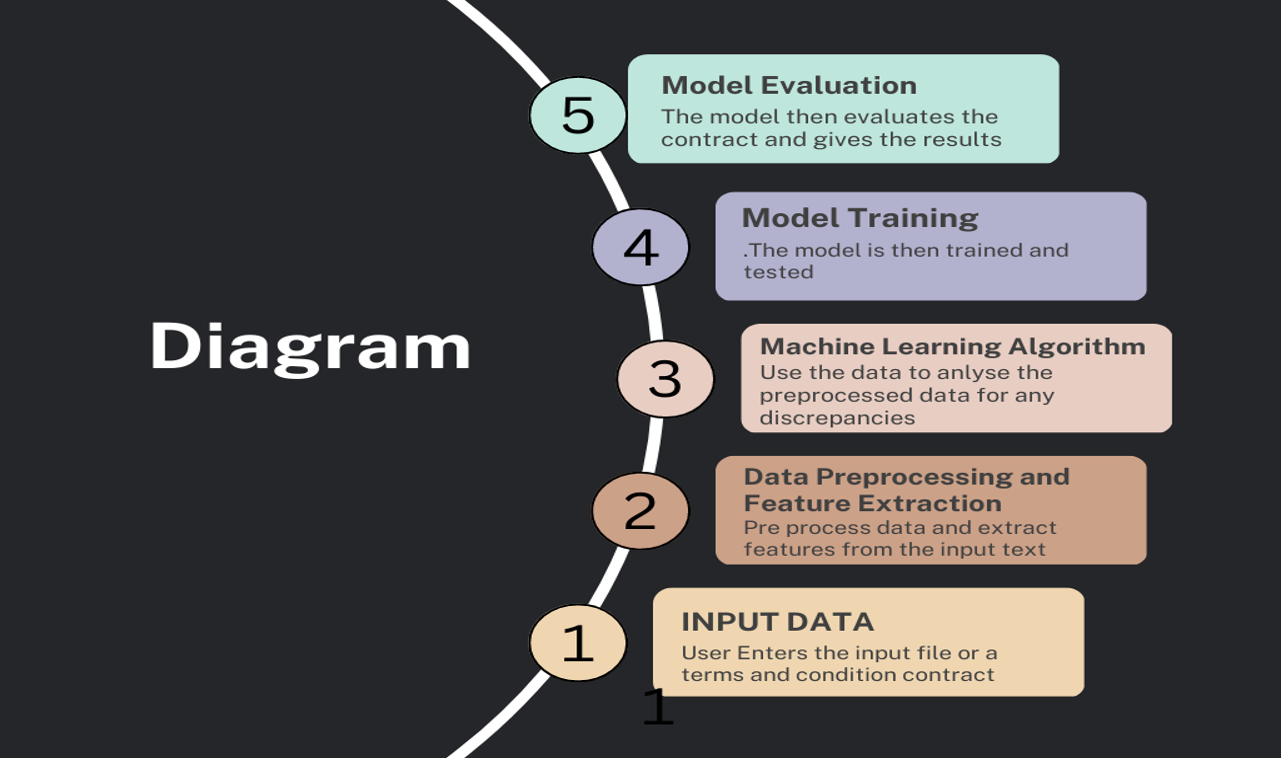
\includegraphics{Figures/Diagramoftheproposedsystem.png}}
\caption{\label{Figure::Diagram Of The Proposed System} Diagram Of The Proposed System  \ref{Figure::Diagram Of The Proposed System}}
\end{figure}





\newpage

\section{Mission Statement \label{Section::Mission Statement} }
The primary purpose of this project is to protect stakeholders from falling victim to deceptive clauses in contracts that may undermine their best interests, either intentionally or unintentionally or via other disruptive means. These clauses could cause harm to the signing party through various means, such as monetary loss or other negative consequences that may impact the livelihood of the concerned stakeholder as a whole. 
The proposed machine learning software system aims to detect and flag such fraudulent clauses in terms and conditions contracts, thus empowering stakeholders to make informed decisions before committing to an agreement. 
By leveraging advanced machine learning algorithms, the system will analyze and identify potential risks in the contract language. This approach ensures that stakeholders are aware of any hidden or obscure terms that could be detrimental to their interests. In addition to enhancing the transparency of contractual agreements upheld in a court of law, the software will enable users to negotiate better terms, minimize potential disputes, and ultimately establish a more secure and trustworthy contractual environment.
\chapter{Scope \\
%\small{\textit{-- Team-11}} 
\index{Chapter!Scope}
\index{Scope}
\label{Chapter::Scope}}



\section{Identification\label{Section::Project Identification} }


\section { Document Overview \label{Section::Document Overview} }



\section{System Overview\label{Section::System Overview}}
% The primary goal of this project is to develop a machine learning model that assists stakeholders in avoiding deception by clauses in terms and conditions (T\&C ) contracts. This approach will automatically analyze all clauses within the contract, providing stakeholders with the necessary information to decide whether to proceed or not.
% Several popular machine learning libraries, such as scikit-learn \cite{scikit-learn}, the Natural Language Toolkit (NLTK) \cite{nltk}, and Keras \cite{keras}, will be utilized to create the model. Flask \cite{flask} and Django \cite{django} will be employed to develop the web application, enabling users to upload T\&C contracts in text or PDF formats and evaluate the presence of any deceptive clauses. Scikit-learn, NLTK, and Keras are widely used libraries for machine learning tasks.
% We will start by selecting a dataset of T\&C contracts that have been identified as containing fraudulent or unclear clauses. The scikit-learn and Keras libraries will be used for feature extraction, where we can extract relevant information from the text. After extracting the features, we can use them to train a machine learning AI model using the scikit-learn engine.
% Once the AI model is trained, it can be evaluated using the Keras library to determine its accuracy. If the model performs well, it can be used to identify whether clauses in T\&C contracts are fraudulent or unclear.
% In summary, this project aims to create a machine learning model that helps stakeholders avoid deception in T\&C contracts by automatically analyzing the clauses within the contract. By using popular libraries and web development frameworks, the model will provide stakeholders with valuable insights and help them make informed decisions about whether to proceed with an agreement or not.

% \begin{figure}
% \centering
% \scalebox{0.53}{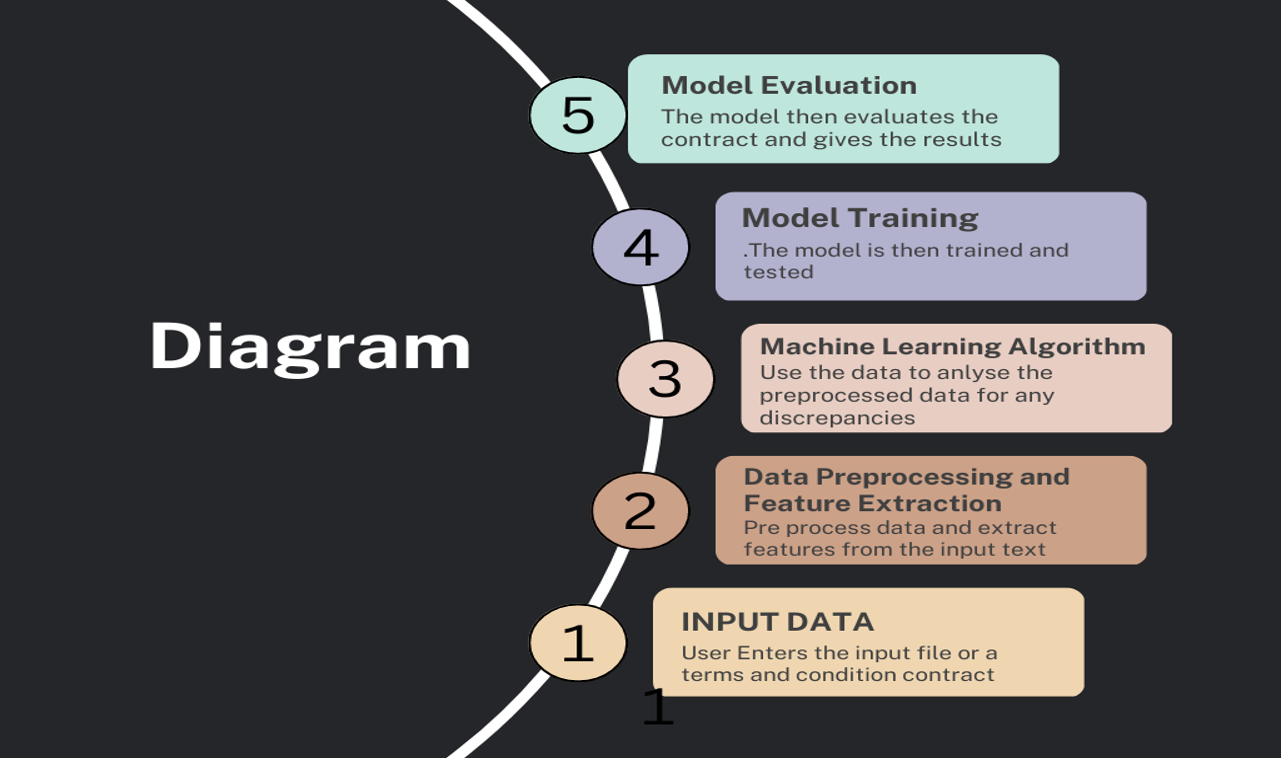
\includegraphics{Figures/Diagramoftheproposedsystem.png}}
% \caption{\label{Figure::Diagram Of The Proposed System} Diagram Of The Proposed System  \ref{Figure::Diagram Of The Proposed System}}
% \end{figure}

\chapter{Referenced Documents \\
%\small{\textit{-- Team-11}} 
\index{Chapter!References}
\index{References}
\label{Chapter::References}}

\begin{itemize}
    \item IEEE Std 1362-1998, IEEE Guide for Information Technology—System Definition—Concept of Operations (ConOps) Document, Approved March 19, 1998.

    \item Dr. Muresan, David Darian. Lecture-5, Lecture-05-Concept Of Operations( ConOps), Stevens Institute Of Technology, 2023
    \item Dr. Muresan, David Darian. Lecture-10, Lecture-10-Requirements Analysis, Stevens Institute Of Technology, 2023
    \item Dr. Muresan, David Darian. Lecture-2, Lecture-2-Stakeholders, Stevens Institute Of Technology, 2023
    \item Dr. Muresan, David Darian. Lecture-3, Lecture-3-Business Requirements, Stevens Institute Of Technology, 2023
    \item Dr. Muresan, David Darian. Lecture-4, Lecture-4-User Requirements, Stevens Institute Of Technology, 2023
    \item Dr. Muresan, David Darian. Lecture-6, Lecture-6- Requirements Elicitation, Stevens Institute Of Technology, 2023
    

    
\end{itemize}
\chapter{Current System Or Situation \\
%\small{\textit{-- Team-11}} 
\index{Chapter!Current System Or Situation }
\index{Scope}
\label{Chapter::Current System Or Situation}}
The motivation behind developing this system is that currently, stakeholders, which in this case would be common person, without much knowledge about the law, are required to manually read through terms and conditions contracts which can often be super long, time consuming and notoriously confusing due to the amount and complexity of the legal terms used, that are at the end of the day, accepted in a court of law, which would be unfamiliar to a common person thereby, risking themselves of inflicting harm in a shape that may result in financial, personal or mental distress. While the option to consult a lawyer exists, it is not always feasible due to their high costs and availability constraints.

In the absence of an effective tool to navigate this challenging problem, the need for a solution like ClauseGuard became apparent. This system is designed to safeguard stakeholders from potential pitfalls hidden in deceptive clauses. By providing a machine learning-based analysis of contracts, ClauseGuard offers a reliable, user-friendly, and cost-effective alternative to traditional methods of consulting a lawyer, fostering a safer and more transparent contract review process.  

\section{Background, objectives, and scope \label{Section::Background,objectives and scope} }
The current system exists to ensure that stakeholders, typically common individuals, are equipped to agree to the terms and conditions contracts set forth by the initiating party. This process, however, is often lengthy, complex, time-consuming, and challenging for the average person to fully understand the implications of the contract. While professional consultation is an option, the high costs associated with it often render it an unfeasible choice.

The mission of the proposed system, Clauseguard, is to ensure that stakeholders can effectively parse through the terms and conditions contract presented by the initiating party. The ultimate aim is to make stakeholders aware of any deceptive or harmful clauses in the contract, thereby safeguarding them from potential financial, personal, or other forms of harm.
 The scope of the proposed system extends to stakeholders from any background ranging from a common person to a lawyer, govermental agencies and mega corporations who may encounter contractual agreements. The objective is to provide support and enhance their understanding of the contracts they engage with, regardless of the complexity of the legal language involved. 



% The primary purpose of this project is to protect stakeholders from falling victim to deceptive clauses in contracts that may undermine their best interests, either intentionally or unintentionally or via other disruptive means. These clauses could cause harm to the signing party through various means, such as monetary loss or other negative consequences that may impact the livelihood of the concerned stakeholder as a whole. The proposed machine learning software system aims to detect and flag such fraudulent clauses in terms and conditions contracts, thus empowering stakeholders to make informed decisions before committing to an agreement.

% By leveraging advanced machine learning algorithms, the system will analyze and identify potential risks in the contract language. This approach ensures that stakeholders are aware of any hidden or obscure terms that could be detrimental to their interests. In addition to enhancing the transparency of contractual agreements upheld in a court of law, the software will enable users to negotiate better terms, minimize potential disputes, and ultimately establish a more secure and trustworthy contractual environment.

\section { Operational policies and constraints \label{Section::Operational Policies and constraints}}
There are a number of operational policies and constraints that are applied to the proposed system.
\subsection{Operational Policies}
An operational policy can be defined as a general statement of required behaviour. The operational policy of clauseguard is as follows: 
\begin{itemize}
    \item Data privacy is a major cause of concern for the proposed system. Sensitive and confidential information would be shared on an open internet website. As such, the system must ensure that no information is stored on any backend servers in the form of "cookies", "tokens" or any similar data logging services. The system should respect data privacy laws partaining to each individual country and follow guidelines as set forth by that particular country. 
    
    \item The system must explicitly ask stakeholders for their consent for analyzing the submitted documents before using the system. This consent would be devised by a team of professional experts and lawyers so as to not hold the parent organization of clauseguard of any legal ramifications. 

    \item The system must utilize a sophisticated machine learning algorithm that is retrained and updated at intervals of every two months. This ensures that the model stays current with the evolving nature of legal language in contracts, reflecting the latest laws and regulations. Additionally, cross-checking with historical legal data is done during these updates to maintain consistency and accuracy. Periodic reviews by legal experts complement the machine learning model, ensuring its recommendations remain accurate and legally sound.

    \item the system must provide clear explanations for any detected clauses in the Terms & Conditions contracts. These explanations are devised by the system based on the analysis of datasets comprising other legal documents of similar nature and scope. This ensures that users not only receive information about potential issues in the contracts they're reviewing, but also gain an understanding of why these clauses may be problematic.
\end{itemize}

\subsection{Operational Constraints}
An operational constraint is an externally imposed condition that must be observed. The operational constraint of clauseguard is as follows: 
\begin{itemize}
    \item The machine learning algrothim would require extreme amounts of processing power and computational resources, which, on failing to secure, would severely limit the number of contracts that can be analyzed. It can also lead to network wide crashes and instability. 
    \item The model depends on the accuracy of the dataset on which it is trained. Lack of available legal documents can induce severe challenge on the authenticity and accuracy of the model. Some countries do not disclose legal documents into the public domain, thereby severely limiting the use of this model in certain geographic locations. 
    \item The model must be online 24/7 365 days of the week. Lack of server resources can cause an availability constraint. 
    \item The model must comply with data regulations  and privacy laws around the world. This constraint cannot be guranteed across every country, as each country has extremely wide definations of data privacy laws, failing to adhere can cause a ban of this sytem in that particular country. 
    \item The model must handle contracts written in different terminologies and structures used across various different countries. For example, Japanese legal system requires legal documents to start from the right to left. Training the model on many different structures is a significant operational constraint. 
    \item The model must ensure the security of private and sensitive data. This is also a major operational constraint as unethical hacking can lead to significant data leaks. 
    
\end{itemize}

\section{Description of the current system or situation \label{Section::Description of the current system or situation}}
The current system is being built with the primary objective of developing a machine learning model to aid stakeholders in identifying potentially deceptive clauses in terms and conditions (T\&C) contracts. This system functions by automatically scrutinizing all clauses within the contract, thereby equipping stakeholders with crucial information needed to make an informed decision regarding their agreement to the terms.
The system uses several machine learning libraries such as scikit-learn, natural language toolkit(NLTK) and keras for the creation of the model. 

Scikit-learn is a machine learning library in Python that provides tools for data analysis and modeling. In this system, scikit-learn is primarily used for preprocessing the dataset and training the machine learning model. It provides utilities for common machine learning tasks such as feature extraction, text representation, and model evaluation. For instance, scikit-learn's text feature extraction utilities can convert the text data in T&C contracts into a format that can be input to the machine learning model.
Natural Language Toolkit (NLTK) is a library in Python that provides tools for working with human language data (text).  In this system, NLTK is primarily used for tokenization (i.e. breaking up of sentences into each indidual alphabet, white space, special character, symbol etc), stemming (A process to remove the suffix from words such as ing), and lemmatization (converting the word into its root form and reducing the superlative of the word into its equivalent comparative, for example: oldest will be old), which are crucial steps in preprocessing the text data.

Keras is a high-level neural networks API in Python.  
It is used to define and train any kind of deep learning model. In this system, Keras is used to define the machine learning model structure and train the model using the preprocessed dataset.

Flask and Django are web development frameworks in Python.  In this system, Flask and Django are used to build the web application that allows users to upload T&C contracts and get the results from the machine learning model. Flask can handle simpler and smaller loads, while Django can manage more complex and larger loads. The choice between them would depend on the requirements and scalability plans of the system. Flask would be used for the inital build of the system followed by django for a more advanced model. 

The system operates by facilitating users to upload a T&C contract via a web interface, developed using Flask or Django. The uploaded contract undergoes a preprocessing step, where it's transformed into a suitable format for the machine learning model using libraries such as scikit-learn and NLTK.

The preprocessed data is then fed into a machine learning model, constructed and trained using the Keras library. This model evaluates each clause in the contract, assigning a risk score that represents the likelihood of the clause being deceptive or unfair.

The output provided to the user includes highlighted sections of the contract that have been flagged as potentially deceptive, along with a percentage indicator that quantifies the overall risk associated with the contract. For each highlighted section, the system also provides an explanation, derived from the model's analysis, clarifying why the clause was flagged.

With this information, the user is empowered to make an informed decision about whether to sign the contract or not. 
The breakdown of the system is as follows: 
\begin{itemize}
    \item Operational Environment and its characteristics: The current environemtn invloves stakeholders using a web platform to upload their T\&C contract into a web interface. 
    \item Major system components and the interconnection among those components: The system comprieses of a machine learning model that is trained on a vast amount of datasets invlovling legal documents from various bracnches of the law such as crimaal law, corporate law, copyright protect, patent law, etc. The model parses each line in the contract, signals out protential harmful clauses that may seek to cause harm to the signing party in the shape of montery or mental duress, and quantifies the risk carried with the contract signified by a percentage. Furthermore, the model genewrates expplainations for the harmful clauses it has highlighted. 
    \item Interfaces to external systems or procedures: The system can be accessed on any platform, device and operating systems. Similar to chatgpt, an api for the model will be released whcih can be integrated into propirety systems that are otherwise not avaialbe to the general public and are the intellectual property of their respective owenrs. 
    \item Capabilities, functions, and features of the current system: The system's objective is to analayze and interpret complicated legal terms, identifying potentially harmful clauses and providing layman explainations to the user. The system's function includes parsing throug each line of the document, running the parsed text through the machine learning model and generating a small report accessable within the website itself that includes a risk assessment percentage as well as a succint explaination, 
    \item e)                \begin{figure}[H]
    \centering
    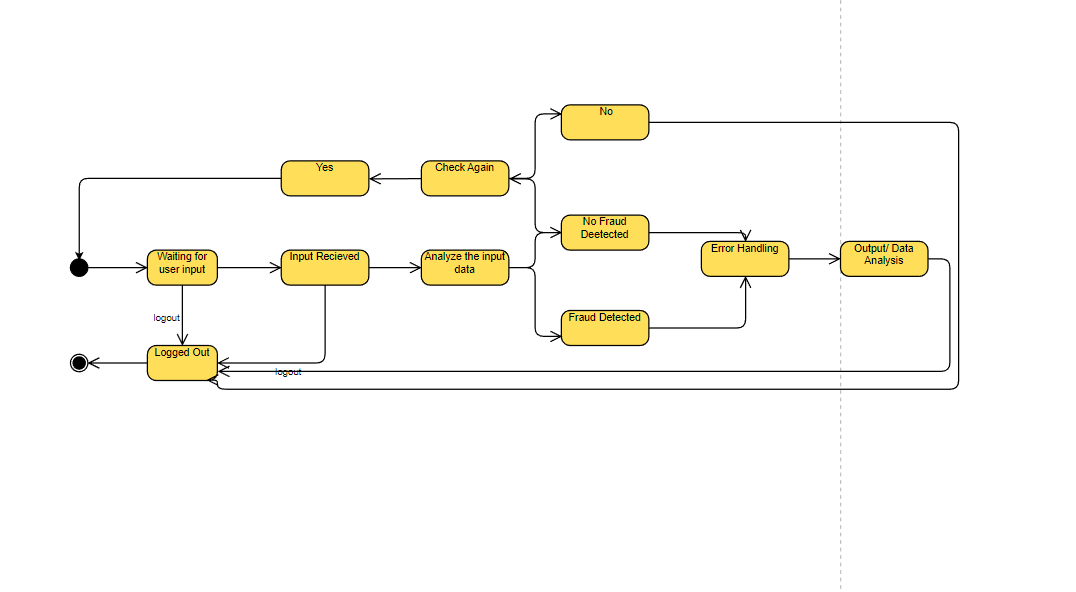
\includegraphics[scale=0.83]{Figures/state machine.png}
    \caption{State Machine View of the diagram \ref{fig:state machine}}
    \label{fig:state machine}
\end{figure}
   

    \item Cost of system operations: The cost of running the system would depend upon the amount of resources that it would take to run the model on servers accessible throughout the world wide web whist analyzing millions of documents concurrently. Load balancers and other such infrastructure must be set up to ensure the working for the model. Infrastructure like the Amazon AWS could be used to set up the model. This would solve the problem with data protection too.  Maintenance would require additional funds. Overall, a cost in the 7 figure range is expected for the initial version of the system 

    \item Operational risk factors: Several operation risk factors could occur which include inaccurate intepretation and explaination, legal reprucssions, confidential Data leaks, Security breaches, server crashes, instability, low accuracy, inaccurate percentages and so on. 
    \item Performance characteristics: The model should be fast, accurate and able to process large quantities of data. To ensure these non-functioanl requirements, the model can be set up on additional infrasture such as could bases services. Amazon AWS would benefit the model tremedously. 
    \item Quality attributes: The model should aim for high availability, reliability and secuity. Becuase of the nature of deleaing with legality of a country, accuracy, avaialbity and reliability are of utomost importance. 
    \item Provisions for safety, security: Due to the nature of the model itself, sensitive and confidential data will be shared. The model must ensure data privacy and secuity of the system to prevent potential breaches and subsequent leaks of confidential data. The system must be designed to ensure high frequency of backed up data to guarantee swift recovery of said data if  operational failures occur. 
\end{itemize}

 



\section{Modes of operation for the current system or situation \label{Section::Modes of Operation for the current system or situation}}
The system will operate on various modes of operation throughout its lifecycle as detailed below: 
\begin{itemize}
    \item Training Mode: This mode is only accessible to the system's developers and not to the end users. It plays a crucial role in the functioning of the system as this is where new features are developed, the model is trained on additional datasets, and existing defects are patched. The training mode uses large amounts of T\&C contracts to train the machine learning model to understand the structure, language, and meaning of various clauses. This process allows the model to learn how to distinguish between benign and deceptive clauses. Enhancements and updates to the system are made in this mode before being deployed to the Operational Mode. 
    \item Operational Mode: This model is the primary end product of the system used by the users to upload T\&C contracts for analysis. The system would use the model developed in the training mode to evaluate the uploaded contract. It identifies potentially deceptive clauses, calculates the overall risk associated with the contract, and provides explanations for flagged sections. The results are then displayed to the user, who can use this information to make an informed decision about whether to sign the contract.
    \item Emergency Mode: This mode serves as a contingency plan, activated in the event that both the Primary and Training modes experience operational failures. The Emergency Mode relies on a legacy version of the currently deployed primary model. This fallback mechanism ensures continuity of service even in the face of unforeseen disruptions. While it may not have the most recent updates and features available in the Primary Mode, the Emergency Mode is designed to effectively analyze T&C contracts and identify deceptive clauses, thereby maintaining the core functionality of the system. Regular checks and minor updates are carried out to ensure that the Emergency Mode is always ready for activation, should the need arise. This robust backup plan contributes to the system's resilience and reliability, offering users a dependable tool for contract analysis at all times.
    


\end{itemize}


\section{User classes and other involved personnel \label{Section::User Classes and other involved personnel}}
Clauseguard would involve the participation several user classes and  personal either directly or indirectly depending upon their interaction with the system as given below: 
\begin{itemize}
    \item End User: The end users are the primary users of clauseguard. They interact directly with the system by uploading the T\&C contracts for analysis. Their interaction is via the web platform, with the aim of identifying deceptive contracts in T\&C contracts. They don't require any skill levels except basic computer skills. 
    \item Developers: They are the primary coders of the system. Their responsibilities include, implementing new features, functionality and maintenance of the system. They require high skill levels in the fields of programming and problem-solving as they require a high level of technical skill and familiarity with the underlying technology.
    \item Machine Learning Specialists: ML specialists work to continually improve clauseguard's machine learning algorithm. They are responsible for training the model on new datasets, testing performance and implementing updates as needed. Their interaction is through machine learning libraries used in the development of the model. 
    \item CyberSecurity Experts: These individuals play a crucial role in safeguarding the ClauseGuard system from unauthorized access and potential security threats and are arguably the most important stakeholders in the functioning of clauseguard as a service. They are tasked with the responsibility of thwarting attempts by unethical entities, often referred to as hackers, who might attempt to breach the system and gain access to confidential data. Cybersecurity experts work diligently to identify and secure any potential vulnerabilities in the system that could be exploited for malicious purposes. Their interaction with the system spans across all areas, but they primarily focus on the system's edge cases and potential weak points that could be susceptible to breaches. They are proficient in the latest cybersecurity protocols and techniques and utilize this expertise to constantly enhance the system's security measures. In addition, they collaborate closely with the system administrators and developers to ensure that security is integrated into all aspects of the ClauseGuard system, from the web application to the machine learning model itself. Their work helps maintain the trust of the end-users by ensuring that their interactions with the system remain secure and confidential.
    \item Legal Consultants: Although their involvement may not be direct, they nevertheless, play a crucial role in the development of the model. They review the machine learning model's output to ensure its accuracy and make recommendations for improvement based on their legal expertise. They interact indirectly with the system by providing feedback and suggestions for model enhancements based on their understanding of legal terminologies and concepts.
    \item Commercial enterprises stand to gain significantly from the use of the ClauseGuard system. These entities often engage in complex transactions that involve extensive legal contracts. With the help of ClauseGuard, they can quickly and efficiently review these contracts, expediting the deal-making process. For instance,  the  purchase of Activision-Blizzard by Microsoft made headlines across the tech industry. In such scenarios, missing or overlooking crucial legal details can lead to considerable impediments, potentially blocking the deal altogether which happened in the case of Microsoft acquiring Activision-Blizzard. ClauseGuard can mitigate such risks by identifying potentially harmful or unclear clauses that could jeopardize the agreement. This can save enterprises substantial time and resources, while also providing them with a layer of protection against contractual pitfalls. Similar to end users, commercial enterprises need only basic computing skills to access clauseguard. 

\end{itemize}


\section{Support environment \label{Section::Support Environment}}
Clauseguard will have a number of support systems in place that will fortify the absolute working of the system to its fullest capacity. 
\begin{itemize}
    \item Clauseguard will have a dedicated technical support team. This team will handle technical queries, troubleshoot reported issues and work on continuous improvement of the system. 
    \item Since clauseguard would primarily be virtual, the equipment and facilities would involve robust server architecture preferbly on cloud bases services such as AWS, load balancers for handling multiple connection requests and IT infrastructure for the support team to handle issues effectively. 
    \item Clauseguard would have a customer service team and infrastructure to manage user inquiries, issues and feedbacks. This platform would involve efficient tracking and resolution of support tickets. 
    \item ClauseGuard , being a cloud-based application, would use secure cloud storage services to store user data and application elements essential for the functioning of the system. It is to be noted that any personal or confidential data will not be stored in any capacity. 
\end{itemize}





\chapter{Justification for and nature of changes \\
%\small{\textit{-- Team-11}} 
\index{Chapter!Justification for and nature of changes }
\index{Justification for and nature of changes}
\label{Chapter::Justification for and nature of changes}}\



\section{Justification of changes  \label{Section::Justification of changes} }
Justification for the changes of the proposed systems is outlined below: 
\begin{itemize}
    \item New or modified aspects: The rapidly changing legal landscape and increasing complexity and ambuity in T\&C contracts propelled the need for an efficent and reliable system that can adapt and and update itself based on the latest laws and guidelines. 
    \item Limitations of the current systems: At the moment, most contracts are manually reviewed by legal professionsals. This process is time0consuming, tedious and prone to error. Furthermore, the interpretation of different terms and conditions may vary between different individuals leading to inconsistancies in evaluations. 

    \subsection{Justification for a new or modified system}
    Clauseguard can effectively counter the challenges faced by the current system as outlined below: 
    \begin{itemize}
        \item With the advent of the COVID-19 pandemic, there has been a significant uptick in the usage of digital contracts. This transition has led to a surge in data volumes that traditional methods of review cannot efficiently handle. ClauseGuard's machine learning model, with its inherent ability to process and analyze vast amounts of data swiftly and accurately, stands to offer an invaluable service in this context. It can help stakeholders navigate through the labyrinth of digital contracts, ensuring they are informed and protected. This capability is not just a convenience; it is a necessity in the rapidly digitizing world, where the velocity and volume of contractual agreements are ever-increasing. 
        \item The machine learning system aims to automate the evaluation of contracts, significantly reducing the time and resources required, thereby leading to lower operational costs. It can also improve consistency in evaluations by reducing subjective human interpretation.
        \item The capability to autonomously detect deceptive or unclear clauses within contracts has become increasingly necessary in today's rapidly evolving legal landscape. Contracts are becoming more intricate and are subject to frequent revisions due to changing regulations and business practices. These complexities often make it challenging for individuals to fully comprehend the terms, leading to potential misinterpretations and unintended commitments. An automated system that can reliably dissect and interpret these complexities not only promotes transparency but also serves as a protective measure for stakeholders. 
    \end{itemize}
    
\end{itemize}


\section{Description of desired changes \label{Section::Description of desired changes}}
Clauseguard has a number of capabilites, interfaces and personel changes which are highlighted below: 

\begin{itemize}
    \item Capability Changes: The implementation of the machine learning model will introduce new capabilities such as automated analysis of T&C contracts, detection of deceptive or unclear clauses, and explanations for detected clauses. While the original system relied on manual inspection and comprehension of contract clauses, the new system will automate this process, significantly reducing the time and effort required to review contracts. Moreover, it would be cost effective for those individuals who otherwise, would not abe able to affort professional legal opinion.
    \item System Processing Changes: The machine learning model process the uploaded contracts, analyze the clauses, and output results indicating the presence of any deceptive clauses along with explanations for the same. 
    \item  Interface Changes: The user interface will be modified to allow users to upload contracts and view results. This interface will need to be intuitive and user-friendly, providing clear instructions on how to upload contracts and view results. Changes to the interface will also need to accommodate the presentation of results, which will now include highlighted clauses and their explanations.
    \item Personnel Changes: The development and maintenance of the machine learning model will require personnel with expertise in machine learning, natural language processing, and contract law. Additionally, user training may be required to educate users on how to interact with the new system and interpret its outputs.
    \item Personnel Changes: The development and maintenance of the machine learning model will require personnel with expertise in machine learning, natural language processing, and contract law. Additionally, user training may be required to educate users on how to interact with the new system and interpret its outputs.
    \item Environment Changes: The implementation of the machine learning model will digitize the contract review process, requiring an operational environment that can support the deployment and use of this technology. This may involve changes to existing IT infrastructure and the adoption of new technologies to support the model.
    \item Operational Changes: The introduction of the machine learning model will fundamentally change how contracts are reviewed traditionally. Instead of manually reading through contracts, users will upload them to the system for analysis. This will change the operational procedures and daily work routines of the users.
    \item Support Changes: The implementation of the machine learning model will necessitate changes in the support requirements. Technical support will need to be available to address any issues that arise with the use of the machine learning model. Moreover, regular updates and maintenance will be required to ensure the model remains up-to-date with changes in contract law.
    \item Other Changes: As a result of the implementation of the machine learning model, there may be changes to the time required to review contracts. As the process becomes more automated, it is likely that contract review times will be significantly reduced, allowing for quicker decision-making, faster legal processes and reduction in the cost of paralegal teams. 














\end{itemize}


\section{Priorities among changes \label{Section::Priorities among changes}}
The proorites for the system ClauseGuard are highlighted below: 
\begin{itemize}
    \item Essential Features: \begin{itemize}
        \item The core feature of the system is its ability to identify and highlight potentially fraudulent clauses within a contract. Without this feature, the system would not serve its primary purpose. Failure to implement this would lead to users not being able to identify potential risks in contracts.
        \item The system should be able to assign a risk percentage to each contract, indicating the level of potential fraud. This is vital as it quantifies the risk involved, aiding users in their decision-making process.


        \item Each identified risk should come with an explanation to help users understand the reasons why the clause has been flagged as fraudulent. Without this feature, users may be left confused about the nature of the risk involved.


       
        




    \end{itemize} 

    \item Desirable Features: 
    \begin{itemize}
        \item While not essential, having an intuitive and easy-to-use interface would greatly enhance user experience, encouraging more frequent use and increasing user satisfaction.

        \item The ability to integrate with common document management systems would make the application more versatile and convenient to use. It would allow users to directly upload contracts for analysis from a wide range of document format systems.

        \item  An ability to analyze and present a comparison of risk percentages. This feature would provide users with an onjective metric along with an explaination of why that specific clause was highlighted intended to allow the user to make an informed decision. The decision, ultimately, is left upto the descretion of the user. 

    \end{itemize}

    \item Optional Features: 
    \begin{itemize}
        \item The ability to process and analyze contracts in multiple languages would increase the usability of the system across different geographic locations and allow for greater control over the scanned documents.
        \item A feature that allows multiple users to view and discuss the same contract in real-time. This can facilitate faster decision-making, especially in larger teams similar to that of what the platform "Overleaf" does for LaTeX documents.
        \item Providing API access would allow third-party developers to integrate ClauseGuard's features into their own applications.
        \item Allowing users to directly sign off on safe contracts via popular e-signature platforms could streamline the contract approval process such as adobe signature. 
        \item A feature that allows users to customize the risk percentage threshold that triggers a flag, enabling a more personalized user experience.
        \item  feature that tracks and displays changes made to a contract over time, helping users see how the risk assessment has evolved.

    \end{itemize}

\end{itemize}




\section{Changes considered but not included \label{Section::Changes considered but not included}}
Some features that were considered for ClauseGuard but were not included as follows: 
\begin{itemize}
    \item A Real-Time Fraud Detection feature would have allowed the system to analyze contracts and detect fraudulent clauses as the user is typing or editing the contract. However, due to the significant computational resources required for real-time analysis and the potential disruption to the user experience due to lag or delay, this feature was not included.
    \item A feature for automatic contract modification which would allow the system to suggest modifications to contracts to eliminate or mitigate the risk of identified fraudulent clauses. However, this was not included due to the potential legal implications and the complexity of accurately generating legally sound contract language.
    \item An AI chatbot feature was considered to provide immediate assistance to users. However, due to the complexity of developing a chatbot that can accurately understand and respond to a wide range of user queries, this feature was not included.




\end{itemize}
Note: Although the above features are not included at this time of development, these are features that could be looked at to add on at a later stage of ClauseGuard's life cycle. 

\section{ Assumptions and Constraints \label{Section::Assumptions and Constraints}}
The assumtions and constraints of clauseguard are as follows:
\begin{itemize}
    \item Assumptions: An assumption is defined as a condition that is taken to be true. Some of the assumptions for ClauseGuard are: 
    \begin{itemize}
        \item Data Availability: We assume that the system will have access to a sufficient number of sample contracts with and without fraudulent clauses for training the machine learning model.
        \item User Literacy: We assume that users have a basic understanding of contractual language and terms, as this will influence how they interact with the system and interpret the risk assessments.
        \item Scalability: We assume that the number of contracts to be analyzed will increase over time as more users adopt the system, necessitating a scalable architecture.
        \item Legal Compliance: We assume that all analyzed contracts will be in compliance with local laws and regulations, which the system will need to be updated to reflect.






    \end{itemize}
    \item Constraints: A constraint can be defined as an externally imposed limitation placed on the new or modified system or the processes used to develop
or modify the system. Some of the constraints of ClauseGuard are as follows: 
\begin{itemize}
    \item Budgetary Constraints: The development and maintenance of the system is subject to the availability of funds. This might limit the number of features that can be implemented at a given time.
    \item Time Constraints: The system must be developed and made operational within a specified timeframe. This could limit the amount of testing and refinement that can be done before launch.
    \item Privacy Constraints: The system must comply with data privacy laws and regulations, such as GDPR. This could limit the type of data that can be collected and how it can be used. The system must also take into account some countires that are cut off from the rest of the world such as Russia, Azerbaijan, Kyrgyzstan etc. 


\end{itemize}
\end{itemize}


\chapter{Concepts for the proposed system \\
%\small{\textit{-- Team-11}} 
\index{Chapter!Concepts for the proposed systems }
\index{Concepts for the proposed system}
\label{Chapter::Concepts for the proposed system}}\



\section{Background, objectives, and scope \label{Section::Background,objectives,and scope proposed}}
The rationale for the proposed approach is that it can be challenging for people to spot fraudulent elements in contracts since they are sometimes buried within lengthy and complicated terms and conditions. The suggested system's goal is to identify dishonest clauses in contracts using machine learning techniques, which will increase the contracts' fairness and transparency for all parties. The proposed system's scope includes contract analysis across a range of industries, including technology, insurance, and financial services.


\section{Operational policies and constraints \label{Section::Operational Policies and Constraints proposed}}
The system must make sure that user data is not abused or disclosed without permission, and that the data it gathers and analyzes is handled securely and confidentially.
The system must be precise and trustworthy in spotting contract fraud. The algorithms and outcomes of the system must be rigorously tested and validated for this.


\section{Description of the proposed system \label{Section::Description of the proposed System proposed}}
To find potentially dishonest clauses in contracts, the suggested method will employ machine learning algorithms and natural language processing. Contracts will be analyzed by the system, and any clauses that seem to be unfair, misleading, or deceptive will be flagged. The system will also explain its findings so that consumers may comprehend the justification for the system's choices.



\section{Modes of operation \label{Section::Modes of operation proposed}}

The suggested system will function in two different ways:

In manual mode, a user can upload a contract to the system for analysis, and the system will then give that analysis.

Real-time mode, when the system continuously checks contracts for dishonest clauses and alerts the user to any potential problems.


\section{User classes and other involved personnel \label{Section::User Classes and other involved personnel proposed}}
People and organizations involved in contract formulation and approval will make use of the suggested system. These professionals working with contracts include attorneys, contract managers, compliance officers, and others. Additionally, the system will work with specialists in machine learning who will be in charge of enhancing and refining the system's algorithms.


\section{Support environment \label{Section::Support Environment proposed}}
User guides, online help, and a customer service team will all be part of the support system for the planned system. The system will also include a feedback tool that will let users comment on how well the system is working and recommend changes. To guarantee that the system is operating at its peak performance, routine upgrades and maintenance will be offered.



\chapter{Operational scenarios 
%\small{\textit{-- Team-11}} 
\index{Chapter!Operational scenarios }
\index{Operational scenarios}
\label{Chapter::Operational scenarios}}\

A scenario can be defined as a  step-by-step description of how the proposed system should operate and interact with its users and its
external interfaces under a given set of circumstances. The operational scenario for the following proposed system is outlined below
\begin{itemize}
    \item Normal Operation Scenario: The user navigates to the website, facilitated by a user-friendly interface designed for ease of use. They are greeted by clear instructions and prompts guiding them to upload a Terms and Conditions (T\&C) contract. This can be in various formats such as text, PDF, or LaTeX document, providing ample flexibility to the user.

Once the contract is uploaded, the system initiates the preprocessing stage. This involves cleaning and formatting the text data, utilizing Natural Language Processing techniques such as tokenization, stemming, and lemmatization. This step ensures that the machine learning model receives the data in a suitable format for analysis.

Upon completion of the preprocessing stage, the data is fed into the machine learning model, which has been trained on a vast dataset of T\&C contracts. The model thoroughly scrutinizes the clauses in the contract, identifying any potential deceptive or unclear clauses.

The user then receives a comprehensive report, detailing the analysis results. The report includes a percentage counter indicating the proportion of potentially deceptive clauses found in the contract. Each flagged clause is highlighted, and clicking on it provides a brief explanation as to why it was flagged by the model.

With this detailed insight, the user is better equipped to make an informed decision on whether to proceed with the contract. To proceed with the contract, is left upto the discretion of the user. 

\item Stress handling scenario: A stress handling scenario occurs in a situation where multiple users simultaneously access the website, potentially leading to the analysis of millions of documents concurrently. In such high-demand situations, the system is designed to maintain operational efficiency, ensuring that all users receive a timely and accurate analysis of their contracts.

To manage this high traffic, the system utilizes a sophisticated load balancing mechanism. This mechanism dynamically allocates system resources to different tasks based on demand, ensuring that no single task is overburdened. The load balancer distributes the workload across various system servers located on strategic geographic locations, preventing any bottlenecks or system slowdowns.

Furthermore, the system is built with scalability in mind. It has the capacity to ramp up resources when demand surges, such as during peak usage hours. This ensures that even in times of heavy load, the system remains responsive and continues to deliver results promptly.

Lastly, the system employs robust error handling techniques. In the rare event of a failure or error, the system is designed to recover gracefully, minimizing the impact on the user. Alerts are sent to the system administrators to ensure rapid response and resolution.

Through these measures, the system can effectively manage stress scenarios, providing reliable, efficient service to all users, even during periods of peak demand.

    \item Error handling Scenario: An error handling scenario comes into play when a user attempts to upload a contract in an unsupported file format. In such a situation, the system is designed to promptly identify the issue and respond appropriately and in a timely manner.

Upon detecting an unsupported file format, the system triggers an error message. The system informs the user that the uploaded contract file format isn't supported and kindly prompts them to upload the contract again in a compatible format.

In addition, this error message includes a list of the supported file formats for the user's convenience. This  approach not only resolves the issue at hand but also educates the user about the correct file formats, preventing the same error from reoccurring in the future.

Furthermore, the system logs this error in a database. These logs are periodically reviewed by the system administrators to identify patterns and potential areas for system improvement. For instance, if a particular unsupported file format is frequently attempted by users, the team may consider adding support for that format in future system updates.

Thus the error handling scenario is designed to be user-centric in its approach and its commitment to provide a seamless, intuitive user experience. 

 \item Degraded Operation Scenario: A system degradation scenario comes into play when there's an unforeseen failure with the primary system. In such instances, our robust backup strategy ensures that service continuity is maintained, albeit the service may not be as robust as the primary model.

Upon detection of a primary system failure, the system automatically transitions to a legacy version. This redundancy plan allows users to continue accessing the system and uploading contracts for analysis, ensuring that the primary functionality of the system. remains available. This would also ensure that there is no monetary loss to the organization in the event of a catastrophic system failure. 

However, its important to note that while the legacy system is fully functional, it might not match the performance, accuracy, or feature set of the primary system. As it is an older version, it may process contracts more slowly, and its clause analysis might not reflect the most recent legal developments or algorithmic improvements.

During this degraded mode operation, users will be informed about the temporary switch to the legacy system via a notification on the website. This message reassures them that services are still operational, but also sets appropriate expectations about the temporary limitations they might experience.

Meanwhile, our dedicated team of technicians would be alerted to the issue and would begin troubleshooting the primary system. The goal would be to restore the primary system to full functionality as quickly as possible to minimize the time users spend operating under the degraded mode.

This degradation scenario works towards highlighting our commitment to service reliability and continuity. We understand that our users depend on our system, and we have contingency plans in place to ensure that unexpected issues don't interrupt the availability of our services.

    \item Emergency scenario: In the event of a security breach, our system swiftly transitions to a minimally functioning mode to prioritize data protection and system integrity.

Upon detecting a potential security threat, our system automatically triggers its emergency protocol. This protocol includes limiting user access, suspending non-essential operations, and activating enhanced security measures. The aim is to isolate the breach, protect sensitive data, and prevent further unauthorized access to ensure no confidential or sensitive data is leaked.

During this emergency mode, users may encounter restricted functionality. Access to majority of the services might be temporarily suspended , and the overall system performance may be reduced. However, these measures are critical to maintaining the security of the system and safeguarding user's data.

Simultaneously, our cybersecurity team would be alerted to the situation. These experts would immediately initiate an investigation into the breach, working tirelessly to neutralize the threat and restore the system to full functionality. Users would be notified about the situation and would be kept informed about progress towards resolution.

This emergency scenario highlights our commitment to data security and system integrity. We understand the critical importance of protecting sensitive information, and our system is designed to respond effectively to any security threats, minimizing potential damage and disruption.

    \item Backup Scenario: In circumstances where data integrity is compromised, due to a security breach, system error, or data corruption, or unethical stakeholders trying to  gain access, the system would resort to its backup protocols to ensure data preservation and service continuity.

Our system routinely creates secure backups of all operational data. These backups are securely encrypted and stored off-site to ensure data safety. The frequency of these backups is decided based on the criticality and volume of the data, ensuring minimal data loss in case of unexpected events.

Upon the detection of any data corruption or loss, the system triggers its backup recovery procedure. The most recent unaltered backup is identified, and the data is seamlessly restored to the system. During this process, the system may operate in a limited capacity to ensure the stability and accuracy of the data restoration process.

Meanwhile, our dedicated teams would work on identifying and rectifying the cause of the data loss or corruption, making sure the same issue does not recur. Users are kept informed of the situation and provided with any necessary guidelines or precautions to ensure their data safety.

This backup scenario is an integral part of our commitment to providing a reliable and secure service.
    \item Maintenance Scenario: In the interest of continuous improvement and to ensure optimal performance, the system is periodically placed into a maintenance mode. During these scheduled maintenance periods, updates are performed, enhancements are made, bugs are addressed, and routine checks are conducted to ensure the overall health and security of the system.

These maintenance events are carefully planned and scheduled during periods of expected low usage to minimize inconvenience for our users. Advance notifications are sent to users to inform them about the maintenance schedule and the expected duration of downtime. The importance of the service is understood and the every effort is being made to keep these periods as brief as possible.

During maintenance, the system might be temporarily unavailable or operate with limited functionality. However, these periods are crucial for implementing system upgrades, installing security patches, and performing hardware checks, all aimed at providing a seamless, secure, and efficient service.

Upon completion of maintenance, the system returns to its normal operational state. Users are promptly notified that they can resume using the service as usual. Our dedicated support team remains available to address any queries or concerns users may have post-maintenance.

This maintenance scenario is vital to maintaining the high standards of our system, safeguarding data, and offering an enhanced user experience. It reflects our commitment to delivering a reliable, secure, and up-to-date service to all our users.
\end{itemize}



\chapter{Summary of impacts \\
%\small{\textit{-- Team-11}} 
\index{Chapter!Summary of impacts }
\index{Summary of impacts}
\label{Chapter::Summary of impacts}}\
The proposed system "clauseguard" will have significant operational impacts on users, developers, and the support and maintenance organizations. 
For users, particularly legal and paralegal teams, the system seeks to induce change into the fundamentals of the existing workflow. Instead of manually reviewing contracts, users will now have the ability to upload them to the system and then analyze the generated reports to identify potentially fraudulent activities along with the explanations. This is expected to reduce the time spent on contract reviews, thereby increasing productivity and allowing more focus on complex cases that require human intervention.

Developers will face a shift in their roles as they will have to maintain and update the machine learning model regularly. This includes ensuring that the model is trained on up-to-date data, optimizing it for better performance, and resolving any issues that might arise.
Support and maintenance organizations will  need to familiarize themselves with the working of the ClauseGuard system. They will have to handle new kinds of queries and issues that may arise from the system's operation. The organizations will also have to develop a robust data backup and recovery system to protect the data fed into ClauseGuard.
It is to be noted that although these impacts are anticipated or expected, they might change over time during the actual implementation of the system.







\section{Operational impacts\label{Section::Operational Impacts}}
Operational impacts can be defined as how the system would evolve to become part of the new operational environment. The operational impacts are highlighted below: 
\begin{itemize}
    \item Since the model is platform independent, interfaces with primary or alternate computing platforms are not required except in the case of data recovery programs. 
    \item The procedure for reviewing contracts will change, as the model will be able to flag potentially deceptive clauses, speeding up the review process and reducing the burden on legal personnel.

    \item The model will require a database of contracts and legal clauses to function optimally. This data may be obtained from existing contract databases, open source legal databases, and other relevant sources.

    \item The system will now require digital versions of contracts to be input for analysis, which may increase the volume of data being handled. 
    \item Due to the need to train and improve the model, there may be changes in data retention policies, especially for contracts and related legal documents.

    \item Investment will be required for the development, implementation, and maintenance of the system, as well as additional cloud infrastructure required to effectively scale the system and ensure maximum availability to the tune of 99.999%  .
    \item While the system is expected to reduce the risk of entering into contracts with deceptive clauses, there may be new risks associated with data security and system reliability as well as the accuracy as existing laws are changed to support the ever evolving landscape of the legal world. 






\end{itemize}




\section{Organizational impacts \label{Section::Organizational Impacts}}
Organizational impact can be defined as the impact on the stakeholders of the system. The impact can be direct or indirect, positive or negative. The breakdown of organizational impact is given below: 
\begin{itemize}
    \item Legal personnel will need to review flagged clauses, in order to improve the accuracy of the model as their input determines the effective working of the model. 
    \item It personnel will have responsibilities for maintaining the system. 
    \item Positions related to manual contract review may be reduced, while positions related to system support and maintenance may increase as well as cloud infrastructure specialists and DevOps engineers. 
    \item Existing personnel will need to be trained to use the system and understand its outputs.

    \item There may be increased demand for personnel with skills in machine learning and contract law. Some personnel may need to be relocated to roles where these skills are more needed and where the model is being actively developed. 
    \item In case of an emergency or disaster that disrupts normal operations, contingency plans will need to be put in place. This will require a subset of personnel who are trained in operating the system to be available to set up and manage operations at an alternate site.

The number of personnel required will depend on the complexity of the system and the volume of contracts that need to be reviewed during the contingency operation. Given the technical nature of the system, these personnel should have a good understanding of machine learning principles, the specific model used, and the legal knowledge necessary to interpret the system's output.

Having a well-trained, technically competent contingency team will ensure that contract review can continue with minimal disruption, even under less than ideal circumstances. This is particularly important given the potential legal and financial implications of contracts with deceptive terms and conditions.




\end{itemize}




\section{Impacts during development\label{Section::Impacts During Development}} 
The impact of the system ClauseGuard during development is as follows detailed below: 
\begin{itemize}
    \item Users, developers, legal consultants, and support personnel will need to be involved in discussions and studies to define system requirements and objectives. The aforementioned stakeholders must be in consensus for the effective development of the system. Induced constraints by the way of conflicting requirements should be avoided at all costs to mitigate the risk of stalled development. 
    
    \item Users and support personnel will need to be involved in reviews and demonstrations of the system, to ensure it meets the organization's needs. They should receive additional training to ensure the maximum efficiency of the system. 

    \item During development, the new system may need to be run in parallel with existing procedures to ensure no disruption to contract review processes.



    \item System testing may require additional resources and may impact normal operations, as potential bugs and issues are identified and fixed.







\end{itemize}







\chapter{Analysis of the proposed system \\
%\small{\textit{-- Team-11}} 
\index{Chapter!Analysis of the proposed system }
\index{Analysis of the proposed system}
\label{Chapter::Analysis of the proposed system}}\

The system "Clauseguard" provides several benefits which are highlighted below: 
\begin{itemize}
    \item The "ClauseGuard" system mundanes access to legal advice, bringing complex knowledge of terms and conditions contracts to the fingertips of the everyday user. By leveraging advanced machine learning algorithms, it empowers individuals and organizations with the ability to identify potentially fraudulent clauses without the need for extensive legal consultation.

" 
    \item By automating the examination process, "ClauseGuard" drastically reduces the margin of human error that may occur even with the involvement of experienced legal consultants. The model's capacity to scan vast amounts of data ensures a thorough, comprehensive review of contractual content, which traditionally could take considerable time and resources.
    \item The system is designed with user-friendliness at its core, making it accessible to any stakeholder with basic computational skills. This opens up the domain of legal understanding, traditionally seen as complex and out of reach for many, to a broader audience. It democratizes the process of understanding and evaluating legal contracts, thereby helping users make more informed decisions.
    \item "ClauseGuard" not only brings about significant cost savings but also enhances the speed and efficiency of contract reviews. It can be utilized by small businesses, corporations, and individual users, thereby promoting a culture of transparency and fairness in contractual agreements.
    \item The system's flexibility allows it to adapt to varying legal environments and contract structures. This means that as legal language and contract formats evolve, "ClauseGuard" can be updated and trained to understand these changes, ensuring it remains a valuable tool for contract review.

    \subsection{Limitations}
    Despite the advantages clauseguard brings to the everyday world, it also has certain limitations which are highlighted below: \begin{itemize}
        \item The performance of the model is contingent on the quality of the data it's trained on. Poor quality data can result in inaccurate detections.
        \item As legal language and fraud strategies evolve, the model will need continuous updates and training to maintain its effectiveness.
        \item As clauseguard is being deployed on an international scale, this presents with a unique set of challenges. Given the varying legal definitions and structures across different countries, the system must be equipped to incorporate a vast array of terminologies and documents. The complexity of the task is amplified by the intricate and distinctive nuances of legal language in different jurisdictions. The system's ability to effectively interpret and adapt to these differences is crucial in its functionality and effectiveness.


        \item  "ClauseGuard" must not only recognize nuances but also articulate them to the user in a comprehensible manner. Translating complex legal jargon into user-friendly language is no simple task, particularly when considering the diverse and intricate nature of legal contracts. This translation process, however, is essential to meet the system's goal of making legal knowledge accessible to the common man.
        \item It is also extremely important to note the potential ethical implications of an automated system providing legal advice. While clauseguard is designed to identify potentially deceptive clauses, it's not a replacement for professional legal advice. The model must be clear in communicating its role as a supportive tool rather than a definitive legal authority.
        




        
    \end{itemize}

\subsection{Advantages}
        Clauseguard provides several key advantages. 
        \begin{itemize}
            \item The system can easily scale to handle larger volumes of contracts without a proportional increase in resources or time.
            \item Unlike human reviewers, "ClauseGuard" offers consistent performance, unaffected by factors like fatigue or bias.


        \end{itemize}
        \subsection{Disadvantages}
        Clauseguard has some disadvantages. 
        \begin{itemize}
            \item Potential for False Positives/Negatives: The model may occasionally flag non-fraudulent clauses as fraudulent (false positives) or miss fraudulent clauses (false negatives).
            \item There can be significant initial costs associated with setting up the system and training the model.
            \item The efficiency of ClauseGuard is directly proportional to the quality of data it receives. If the input data is poorly written or ambiguous, the model's ability to accurately detect deceptive clauses could be compromised.

            \item  While machine learning models can analyze and draw conclusions from vast amounts of data, they lack the human capacity for intuition and contextual understanding. There might be cases where human judgment could provide more nuanced interpretations of contract clauses upheld in a court of law.
            \item The potential for misuse or over-reliance on ClauseGuard could lead to legal liability issues. If a user were to take action based on the model's suggestions and suffer negative consequences, it might raise questions about who is legally responsible.
            \item ClauseGuard may not be fully effective for highly specialized or unique contracts that deviate from standard terms and conditions. Its performance may be limited in such cases.
            \item If ClauseGuard stores or processes sensitive contract data or confidential information, it could raise privacy concerns. Safeguarding user data would be a major responsibility and potential challenge.
            \item The model needs to be continually updated to stay current with changing laws, regulations, and contract norms. This could require significant resources over time.













        \end{itemize}
    \subsection{Alternatives and Trade-Offs Considered}
    Alternatives considered include continuing with manual review of contracts or expert paralegal terms. However, these options do not offer the same level of scalability and consistency, cost effectiveness and availability as ClauseGuard. The main trade-off is the initial investment in time and resources to set up and train the model, balanced against the long-term benefits in efficiency, accuracy, and cost savings.





        
\end{itemize}


\section{Summary of improvements \label{Section::Summary of Imporvements }}
The summary of benefits of clauseguard is as follows: 
\begin{itemize}
    \item New Capabilities: ClauseGuard introduces several  features, with main primary objective being the automated detection of potentially deceptive clauses in terms and conditions contracts. Th is capability is not typically found in traditional contract review processes, which often rely on manual review by legal professionals. Moreover, ClauseGuard can analyze vast quantities of contract data in a fraction of the time it would take a human reviewer, thus increasing efficiency. It also provides legal advice in the fingertips of the ordinary user thereby providing an expert opinion which would otherwise be financially stressful for the common person. 

    \item Enhanced Capabilities: For organizations already employing some form of contract review, ClauseGuard enhances these capabilities by adding a layer of machine learning-based analysis. This technology can identify patterns and anomalies that might be overlooked by human reviewers, leading to a more thorough and robust contract review process. 
    \item Deleted Capabilities: As ClauseGuard"becomes more prevalent, some obsolete or less efficient methods of contract review may be phased out. For example, labor-intensive manual reviews of every clause in a contract may no longer be necessary, saving time and resources. Paralegal teams may be downsized, saving firms specializing in matters of legal representation millions of dollars in added costs. 
    \item Improved Performance: ClauseGuard offers significant performance. Its response time is significantly faster than manual contract review, which can expedite contract negotiations and other business processes. The model's machine learning capabilities also mean that it can continually learn and improve over time, potentially leading to better quality contract reviews. Furthermore, as it's a digital tool, it does not require physical storage space, reducing resource requirements. It can also handle large volumes of data, which might be impractical for human reviewers especially on a time constraint.




\end{itemize}


\section{Disadvantages and limitations \label{Section::Disadvantages and Limitations}}
While the ClauseGuard system brings several significant improvements to the process of understanding legal ramifications of contracts, there are also potential disadvantages and limitations to consider: 
\begin{itemize}
    \item The introduction of ClauseGuard may necessitate retraining for personnel who are accustomed to traditional contract review methods. This training could involve understanding how to operate the system, how to interpret its output, and how to troubleshoot any issues that may arise. The time and resources required for this retraining could be significant, especially in larger organizations. 
    Note: This is similar to retraining of many writers, and experts after the advent of "ChatGpt" in many workforces. Writers and editors are being retrained as "Prompt Engineers". These engineers are being trained on utilizing OpenAI's ChatGPT to write stories, fix grammatical mistakes and editing issues without the need for manual review. It is also causing significant loss to jobs in the fields of journalism, content writing and publishing. We expect the outcome with the introduction of clauseguard.
    \item The adoption of ClauseGuard might also entail a change in workflow or workspace organization. For instance, legal teams may have to adjust their work processes to integrate the output of the system into their contract review and negotiation procedures.
    \item While ClauseGuard is designed to detect deceptive clauses, it may not encompass all the features desired by users. For instance, it might not fully understand and interpret highly nuanced or complex legal language that varies from one jurisdiction to another.
    \item The adoption of ClauseGuard may lead to a certain degree of dependence on the tool, which might degrade existing capabilities, especially if personnel become less engaged in manual review processes.








\end{itemize}



\section{Alternatives and trade-offs considered \label{Section::Alternatives and trade-offs considered}}
During the development of clauseguard, we considered several trade-offs in our approach. These are discussed below: 
\begin{itemize}
    \item An initial consideration was whether to employ a rule-based system, where predefined rules are used to detect deceptive clauses, or to utilize a Machine Learning approach, where the system learns to identify such clauses based on patterns in the data.

Trade-offs:  A rule-based system could potentially be more understandable and easier to implement whilst maintaining the nuances of complicated legal jargon,  it would lack the flexibility and adaptability of an ML model to cover the changing legal landscape. It would also require extensive manual input for  development and maintenance.

Decision Reached: We decided to proceed with a Machine Learning model due to its superior adaptability and ability to handle vast and complex contract data as well as designing it to ensure it covers the latest changes in the legal landscape set forth by governments. 


\item Another alternative considered was whether to use supervised or unsupervised learning methods. Supervised learning would involve training the model on a labeled dataset of contract clauses, where deceptive clauses are pre-identified. On the other hand, unsupervised learning would not require pre-labeled data and instead would look for patterns and anomalies in the data to detect potentially deceptive clauses.
Trade-offs: While supervised learning could lead to a more accurate model if high-quality labeled data is available, it requires considerable effort to prepare such data. Unsupervised learning, meanwhile, can handle unlabeled data, making it potentially more scalable, but it might not be as accurate in detecting deceptive clauses.
Decision Reached: A supervised learning approach was chosen because of its potential for higher accuracy and the availability of a sufficient amount of pre-labeled contract clause data.


\item The third alternative considered for ClauseGuard was the choice of going for a web-based platform or an application centric platform. A web-based platform would allow users to access ClauseGuard through web browsers on various devices, including desktop computers, laptops, tablets, and smartphones. It would provide a consistent user experience across different devices and operating systems. Whereas, A application centric would provide users with a dedicated application either on desktop or mobile devices leveraging the  capabilities of their respective operating system and offering offline functionality to those in regions where always online requirement is difficult to obtain.

Trade-Offs: While a application centric approach would be safer, more secure and easier to develop, a web-based platform will guarantee that any stakeholder can access ClauseGuard from any geographic location around the world. In the unlikely case that the model is banned in certain geographic locations, the stakeholders can get around to it by the use of A virtual private network (VPN) to access ClauseGuard.

Decision Reached: After careful consideration, it was decided that a web-based platform would be the preferred approach for developing the model. Stakeholder feedback  indicated a significant preference for accessing ClauseGuard through a web-based interface rather than dedicated applications. This approach aligns with the goal of providing a user-friendly and easily accessible platform.














\end{itemize}





\chapter{Notes 
%\small{\textit{-- Team-11}} 
\index{Chapter!Notes }
\index{Notes}
\label{Chapter::Notes}}\

\chapter{Appendices 
%\small{\textit{-- Team-11}} 
\index{Chapter!Appendices }
\index{Appendices}
\label{Chapter::Appendices}}\


\begin{itemize}
        \item Appendix A: Diagram of the proposed system
        \begin{itemize}
            \item Description: The provided diagram illustrates the proposed system's operational workflow for ClauseGuard, our contract analysis tool. It encompasses a five-step process that clearly delineates the entire functionality of the system.
            \begin{itemize}
                \item Document Upload: The user initiates the process by uploading a legal document for analysis. This is an interactive step where user participation is critical.

                \item Preprocessing: Following the upload, the system undertakes a preprocessing phase. This phase involves cleaning and formatting the raw text of the uploaded document to ensure it's in a format suitable for subsequent analysis.

                \item Feature Extraction: Post preprocessing, the system extracts essential features from the text. This crucial step allows the machine learning algorithm to identify potential patterns, irregularities, or red flags within the document.

                \item Model Training and Testing: While the document is being analyzed, the machine learning model undergoes continuous training and testing. It refines its ability to detect deceptive clauses and improve overall accuracy and performance.

                \item Contract Evaluation: The model evaluates the contract using the extracted features and the knowledge it has gained from training. It applies learned patterns to the new document, identifying any potentially deceptive clauses.

                \item Result Generation: Finally, the system generates comprehensive results. It highlights potentially harmful clauses, offers an explanation for each flagged section, and presents an overall risk score for the contract.


            \end{itemize}
    \end{itemize}

    \item Appendix B: State Machine diagram of the proposed system. 
        \begin{itemize}
            \item Description: The State Machine Diagram presents a high-level visual representation of the ClauseGuard system's operational flow. This diagram illustrates the progression of the system's state, driven by specific events or conditions, thereby defining the sequence of operations in an easy-to-understand manner.
            \begin{itemize}
                \item Start State: The initial state of the system is a standby mode, wherein the system awaits user input. This state represents the system's readiness to analyze a document.
                \item Document Upload: The transition from the standby mode is triggered by a user action - uploading a document for analysis. Once the file is uploaded, the system initiates the process of analyzing the input.
                \item Document Analysis: The system transitions to the analysis state, where the machine learning model scrutinizes the document. This stage is critical as the model applies its trained knowledge to identify potential deceptive clauses.
                \item Branching States - Fraud Detected or Not Detected: Upon completion of the analysis, the system transitions into one of two states, depending on the model's findings.
                \begin{itemize}
                    \item Fraud Detected: If potentially deceptive clauses are identified, the system transitions to a state where these findings are displayed to the user. The user is provided with highlighted sections of the document and explanations for the flags. Upon reviewing the results, the user can choose to exit the checking process or proceed to analyze another document.
                    \item No Fraud Detected: If no deceptive clauses are found, the user is informed of the positive outcome and can choose to exit or continue with the analysis of another document.
                    
                \end{itemize}
                \item Check Again Option: Regardless of the results, the system provides the user with an option to analyze another document. If chosen, the system transitions back to the document upload state, ready to commence a new round of analysis.
            \end{itemize}
The state machine diagram serves as a simplified snapshot of the system's functionality, illustrating the system's behavior and its different states in response to varying inputs. It provides a clear picture of how the ClauseGuard system responds and adapts to user interactions, thereby ensuring a comprehensive understanding of the system's operational flow.



        \end{itemize}
\end{itemize}

\chapter{Glossary 
%\small{\textit{-- Team-11}} 
\index{Chapter!Glossary }
\index{Glossary}
\label{Chapter::Glossary}}\
\begin{itemize}
    \item ClauseGuard: The name of the system being developed. 

    \item ConOps: Abbreviation for Concept Of Operations. 

    \item ML: Machine Learning algorithm that can intelligently perform tasks without explicit coding.
    \item preprocessing: The initial stage in data analysis where raw data is cleaned and transformed to a suitable format for further analysis or model training.



    \item scikit-learn: Python library used for developing the machine learning model. 

    \item NLTK: Natural language toolkit used for preprocessing textual data.  
    \item Keras: A neural network API, used to train the model on preprocessed datasets. 
    \item AWS(Amazon Web Services): A subsidary of amazon providing cloud infrastructre. 
    \item Jira: A proprietary issue tracking product developed by Atlassian that allows bug tracking and agile project management.
    \item GitHub: A web-based hosting service for version control. 

    \item API (Application Programming Interface): A set of protocols, routines, and tools for building software and applications. APIs specify how software components should interact and allow different software systems to communicate with each other.

    \item API (Application Programming Interface): A set of protocols, routines, and tools for building software and applications. APIs specify how software components should interact and allow different software systems to communicate with each other.

    \item ChatGPT: An advanced language model developed by OpenAI, capable of generating human-like text based on the input given to it.

    \item Coverity: A static code analysis tool that helps developers and security teams address security and quality defects early in the software development life cycle.

    \item Velero: An open source tool to safely backup and restore, perform disaster recovery, and migrate Kubernetes cluster resources and persistent volumes.

    \item PDF (Portable Document Format): A file format developed by Adobe in the 1990s to present documents, including text formatting and images, in a manner independent of application software, hardware, and operating systems.
    \item LaTeX: A high-quality typesetting system. It is the de facto standard for the communication and publication of scientific documents.
    \item RTF (Rich Text Format): A proprietary document file format with published specification developed by Microsoft Corporation for cross-platform document interchange with Microsoft products.
    \item GDPR (General Data Protection Regulation): A regulation in EU law on data protection and privacy in the European Union (EU) and the European Economic Area (EEA). It also addresses the transfer of personal data outside the EU and EEA areas.
    
\end{itemize}
\bibliography{bibfile}
%\bibliographystyle{unsrt}
\bibliographystyle{IEEEtran}

%% Initial version by Darian Muresan, Ph.D.
% Edit and adjust as needed.

\documentclass[12pt]{cornell}

% add index support
\makeindex

% graphing programs
\usepackage{color}
\usepackage{psfrag}
\usepackage{verbatim}
\usepackage{fancyhdr}
%\usepackage{titlesec}
\usepackage{fancyvrb} 
% hyperlink programs
\usepackage[pdfmark, 
breaklinks=true, 
colorlinks=true,
citecolor=blue,
linkcolor=blue,
menucolor=black,
pagecolor=black,
urlcolor=blue
]{hyperref} % links in pdf
%\usepackage[colorlinks]{hyperref} % links in dvi
\usepackage{listings}
\usepackage{amsfonts} 
\usepackage{amssymb} 
%\usepackage{tabto}

\usepackage{tabularx,colortbl}
\usepackage[chapter]{algorithm} 
\usepackage{algorithmic} 
\usepackage{blindtext}
\usepackage{imakeidx}


\definecolor{DarkGreen}{rgb}{0,0.6,0}
\definecolor{mygreen}{rgb}{0,0.6,0}
\definecolor{mygray}{rgb}{0.5,0.5,0.5}
\definecolor{mymauve}{rgb}{0.58,0,0.82}

\usepackage{tocloft}
\usepackage{amsmath}
\usepackage{tcolorbox}
\usepackage{enumitem}
\usepackage{longtable}
%\usepackage{textcomp}
\usepackage{txfonts}

%part for \part titles
%chap for \chapter titles
%sec for \section titles
%subsec for \subsection titles
%subsubsec for \subsubsection titles
%para for \paragraph titles
%subpara for \subparagraph titles
%fig for figure \caption titles
%subfig for subfigure \caption titles
%tab for table \caption titles
%subtab for subtable \caption titles

% update chapter number spacing
\setlength{\cftchapnumwidth}{2em}
\setlength{\cftsecnumwidth}{2.5em}
\setlength{\cftsubsecnumwidth}{3.5em}
\setlength{\cftsubsubsecnumwidth}{4.5em}

\addtolength{\cftsecindent}{0.5em}
\addtolength{\cftsubsecindent}{0.5em}
\addtolength{\cftsubsubsecindent}{0.5em}

%\titlespacing*{\chapter}{0pt}{-50pt}{20pt}
%\titleformat{\chapter}[display]{\normalfont\huge\bfseries}{\chaptertitlename\ 
%\thechapter}{20pt}{\Huge}
%\pagestyle{fancy}
%\pagestyle{cornell}
%
%\rhead{F054-021-0172}
%\chead{Nonlinear Enhancement of Visual Target Detection (AF05-T021)}
%\lhead{GSTI}
%\lfoot{\scriptsize Use or disclosure of data on this page is subject
%to the restriction on the title page of this proposal.}
%\cfoot{}
%\rfoot{\thepage}

\newfont{\Bp}{msbm10}
\newfont{\BpBig}{msbm10 scaled\magstep2}
\newfont{\Sc}{eusm10}
\newfont{\ScBig}{eusm10 scaled\magstep3}
\newfont{\Fr}{eufm10}
\newfont{\FrBig}{eufm10 scaled\magstep1}

% some commands:
\newcommand{\dxi}{{\tt m\_xDeltaInput}}
\newcommand{\dyi}{{\tt m\_yDeltaInput}}
\newcommand{\dci}{{\tt m\_cDeltaInput}}
\newcommand{\dxo}{{\tt m\_xDeltaOutput}}
\newcommand{\dyo}{{\tt m\_yDeltaOutput}}
\newcommand{\dco}{{\tt m\_cDeltaOutput}}
\newcommand{\ttf}[1]{{\tt #1}}
\newcommand{\tbl}[2]{{\begin{tabular}{c} #1 \\ #2 \end{tabular}}}

\newcommand{\urltwo}[2]{\mbox{\href{#1}{\tt #2}}}
\newcommand{\qnorm}[1]{\|#1\|_{\bQ}}
\newcommand{\qdot}[2]{\lrb #1, #2 \rrb_{\bQ}}
\newcommand{\kdot}[2]{\lrb #1, #2 \rrb_{\bf k}}
\newcommand{\tdot}[2]{\lrb #1, #2 \rrb}
\newcommand{\mydiff}[2]{\lrb #1 - #2 \rrb}
\newcommand{\lena}{\textit{lena}}
\newcommand{\barb}{\textit{barbara}}
\newcommand{\boat}{\textit{boat}}
\newcommand{\leaves}{\textit{leaves}}
\newcommand{\rings}{\textit{rings}}
\newcommand{\treg}{\textit{train region}}
\newcommand{\dreg}{\textit{denoise region}}
\newcommand{\oreg}{\textit{overlap region}}
\newcommand{\sil}{\sigma_l^2}
\newcommand{\sn}{\sigma^2}
\newcommand{\bn}{{\mbox{\bf \FrBig N}}}
\newcommand{\n}{\mbox{\Fr N}}
%\newcommand{\bn}{\bf N}
%\newcommand{\n}{N}
\newcommand{\bY}{\textbf{Y}}
\newcommand{\bX}{\textbf{X}}
\newcommand{\bb}{\textbf{b}}
\newcommand{\bu}{\textbf{u}}
\newcommand{\bv}{\textbf{v}}
\newcommand{\by}{\textbf{y}}
\newcommand{\bx}{\textbf{x}}
\newcommand{\be}{\textbf{e}}
\newcommand{\bz}{\textbf{z}}
\newcommand{\bs}{\textbf{s}}
\newcommand{\bw}{\textbf{w}}
\newcommand{\bQ}{\textbf{Q}}
\newcommand{\bphi}{\textbf{$\phi$}}
\newcommand{\lsb}{\left[}
\newcommand{\rsb}{\right]}
\newcommand{\lrb}{\left(}
\newcommand{\rrb}{\right)}
\newcommand{\lcb}{\left\{}
\newcommand{\rcb}{\right\}}
\newcommand{\R}{\mbox{\BpBig R}}
\newcommand{\F}{{\cal F}}
\newcommand{\Fk}{\mbox{\Sc F}}
\newcommand{\bQF}{\textbf{Q}_{\mbox{\Sc F}}}
\newcommand{\N}{{\cal N}}
\newcommand{\xlz}{X_l(z)}
\newcommand{\xhz}{X_h(z)}
\newcommand{\xz}{X(z)}
\newcommand{\pr}{ perfect reconstruction }
\newcommand{\smb}{Smith-Barnwell }
\newcommand{\xw}{X(e^{j\omega})}
\newcommand{\xmw}{X(-e^{j\omega})}
\newcommand{\dw}{D(e^{j\omega})}
\newcommand{\dmw}{D(-e^{j\omega})}
\newcommand{\ew}{E(e^{j\omega})}
\newcommand{\emw}{E(-e^{j\omega})}
\newcommand{\fw}{F_0(e^{j\omega})}
\newcommand{\fmw}{F_0(-e^{j\omega})}
\newcommand{\hoz}{H_1(z)}
\newcommand{\hzz}{H_0(z)}
\newcommand{\goz}{G_1(z)}
\newcommand{\gzz}{G_0(z)}
\newcommand{\hzw}{H_{0}(e^{j\omega})}
\newcommand{\hzmw}{H_{0}(-e^{j\omega})}
\newcommand{\hzcw}{H_{0}(e^{-j\omega})}
\newcommand{\how}{H_1(e^{j\omega})}
\newcommand{\homw}{H_1(-e^{j\omega})}
\newcommand{\gzw}{G_0(e^{j\omega})}
\newcommand{\gzmw}{G_0(-e^{j\omega})}
\newcommand{\gow}{G_1(e^{j\omega})}
\newcommand{\gomw}{G_1(-e^{j\omega})}
\newcommand{\wl}{e^{-jwL}}
\newcommand{\aqua}{\textit{AQua with OR }}
\newtheorem{theorem}{Theorem}
\newtheorem{lemma}{Lemma}
\newtheorem{corollary}{Corollary}
\newtheorem{claim}{Claim}
\newtheorem{definition}{Definition}
\newenvironment{proof}{\noindent{\em Proof.}}{\ \hfill Q.E.D.}
%\newtheorem{moduleCount}{L}
\newcommand*{\labelfile}[1]{%
  \label{file:#1}%
}

\lstset{ %
  backgroundcolor=\color{white},   % choose the background color; you must add \usepackage{color} or \usepackage{xcolor}
  basicstyle=\footnotesize,        % the size of the fonts that are used for the code
  breakatwhitespace=false,         % sets if automatic breaks should only happen at whitespace
  breaklines=true,                 % sets automatic line breaking
  captionpos=b,                    % sets the caption-position to bottom
  commentstyle=\color{DarkGreen},    % comment style
  deletekeywords={...},            % if you want to delete keywords from the given language
  escapeinside={\%*}{*)},          % if you want to add LaTeX within your code
  extendedchars=true,              % lets you use non-ASCII characters; for 8-bits encodings only, does not work with UTF-8
  %frame=single,                   % adds a frame around the code
  keepspaces=true,                 % keeps spaces in text, useful for keeping indentation of code (possibly needs columns=flexible)
  keywordstyle=\color{blue},       % keyword style
  language=C++,                    % the language of the code
  morekeywords={*,...},            % if you want to add more keywords to the set
  numbers=left,                    % where to put the line-numbers; possible values are (none, left, right)
  numbersep=5pt,                   % how far the line-numbers are from the code
  numberstyle=\tiny\color{mygray}, % the style that is used for the line-numbers
  rulecolor=\color{black},         % if not set, the frame-color may be changed on line-breaks within not-black text (e.g. comments (green here))
  showspaces=false,                % show spaces everywhere adding particular underscores; it overrides 'showstringspaces'
  showstringspaces=false,          % underline spaces within strings only
  showtabs=false,                  % show tabs within strings adding particular underscores
  stepnumber=1,                    % the step between two line-numbers. If it's 1, each line will be numbered
  stringstyle=\color{mymauve}     % string literal style
  %tabsize=2,                      % sets default tabsize to 2 spaces
  %caption=\lstname                % show the filename of files included with \lstinputlisting; also try caption instead of title
}

% Uncomment draftcopy to get the word DRAFT boldly across the first page
%   By the way, xdvi won't show it but it will come out when you print
%\usepackage[light,all]{draftcopy}		% DRAFT on first page
%\draftcopySetGrey{.97}
%\draftcopyName{Confidential}{150}
%\draftcopFirstPage{1}

% Uncomment drafthead to get the date and DRAFT in the header of pages
% that are normallly numbered on the top, pages 2-n of each chapter for example
% This doesn't work with centered page numbers: \pagestyle{cornellc}
%\usepackage{drafthead}

% Including selective chapters:
% use this to selectively process chapters, etc.  Put a % in front of
% the sections that you don't want done this time.  Includes are
% used instead of \input so that LaTeX will keep track of chapters and
% pages without processing everything.  Don't let any spaces creep in
% around the words or it will not work!


\includeonly{
prologue,
manIntroduction,
projectchoosen,
Scopeaftermain,
References,
Current System Or Situation,
justification,
proposedsystem,
OperationalScenarios,
summary,
AnalysisofProposedSystem,
Appendices,
Notes,
Glossary
}

\makeindex

\begin{document}

\pagenumbering{roman}
\singlespacing
% File: prologue.tex
% Thesis prologue:  Title page, acknowledgements, table of contents,
% list of figures, and list of tables.
%
% this file is to be \include'd after the \begin{document}

% Cornell-style title page
\begin{titlepage}
\centering 
    \title{\textbf{ ClauseGuard: A Machine Learning Software System to Detect fraudulent clauses in terms and conditions contracts }} 
        \author{Team-11 \\ Stevens.edu }
        \conferraldate{}{\today} \maketitle
\end{titlepage}

% Copyright page
%\begin{copyrightpage}
\makecopyright
%\end{copyrightpage}

% Abstract: the abstract body is pulled from the file abstract.tex;
%  the title is pulled from the \title command in the titlepage section
\begin{abstract}
        %\makeabstitle
        \input abstract      % puts the abstract file here
\end{abstract}

\begin{Preface}
\input{Acknowledgements}
\clearpage
    \input Preface.tex
\end{Preface}

% Biographical information pulled from file bio.tex
%\begin{biosketch} \input bio \end{biosketch}

% Dedication (optional):  pulls information from file dedication.tex
%\begin{dedication} 
%\input dedicate 
%\end{dedication}

% Acknowledgements:  pulls information from file acknow
%\begin{acknowledgements} \input acknow \end{acknowledgements}

% Table of contents
\contentspage

% If you have no tables or figures put a % in front of the list page line
% List of tables
\tablelistpage

% List of figures
\figurelistpage



\setcounter{page}{1}        % set page counter
\pagenumbering{arabic}      % set page number style
\pagestyle{fancy}         % top right page numbers
%\pagestyle{cornell}
%\pagestyle{cornellc}       % centered page numbers, disables drafthead

\renewcommand{\chaptermark}[1]{\markboth{#1}{}}
\renewcommand{\sectionmark}[1]{\markright{#1}{}}

\fancyhead{} % clear all fields

\lhead{Chapter \thechapter}
%\lhead{\thechapter}
\chead{\leftmark}
\rhead{\thepage}


\lfoot{Chapter \thechapter}
\cfoot{\copyright Stevens -- \today \mbox{} -- Project Name}
\rfoot{\thepage}

\renewcommand{\headrulewidth}{0.4pt}
\renewcommand{\footrulewidth}{0.4pt}

%\rhead{F054-021-0172}
%\chead{Nonlinear Enhancement of Visual Target Detection (AF05-T021)}
%\lhead{GSTI}
%\lfoot{\scriptsize Use or disclosure of data on this page is subject
%to the restriction on the title page of this proposal.}
%\cfoot{}
%\rfoot{\thepage}


\singlespacing
\include{manIntroduction}
\chapter{Clauseguard \\
%\small{\textit{-- Team-11}} 
\index{Chapter!Clauseguard}
\index{Clauseguard}
\label{Chapter::clauseGuard}}

\section{Project Description\label{Section::Project Chosen}}
The primary goal of this project is to develop a machine learning model that assists stakeholders in avoiding deception by clauses in terms and conditions (T\&C ) contracts. This approach will automatically analyze all clauses within the contract, providing stakeholders with the necessary information to decide whether to proceed or not.
Several popular machine learning libraries, such as scikit-learn \cite{scikit-learn}, the Natural Language Toolkit (NLTK) \cite{nltk}, and Keras \cite{keras}, will be utilized to create the model. Flask \cite{flask} and Django \cite{django} will be employed to develop the web application, enabling users to upload T\&C contracts in text or PDF formats and evaluate the presence of any deceptive clauses. Scikit-learn, NLTK, and Keras are widely used libraries for machine learning tasks.
We will start by selecting a dataset of T\&C contracts that have been identified as containing fraudulent or unclear clauses. The scikit-learn and Keras libraries will be used for feature extraction, where we can extract relevant information from the text. After extracting the features, we can use them to train a machine learning AI model using the scikit-learn engine.
Once the AI model is trained, it can be evaluated using the Keras library to determine its accuracy. If the model performs well, it can be used to identify whether clauses in T\&C contracts are fraudulent or unclear.
In summary, this project aims to create a machine learning model that helps stakeholders avoid deception in T\&C contracts by automatically analyzing the clauses within the contract. By using popular libraries and web development frameworks, the model will provide stakeholders with valuable insights and help them make informed decisions about whether to proceed with an agreement or not.

\begin{figure}
\centering
\scalebox{0.53}{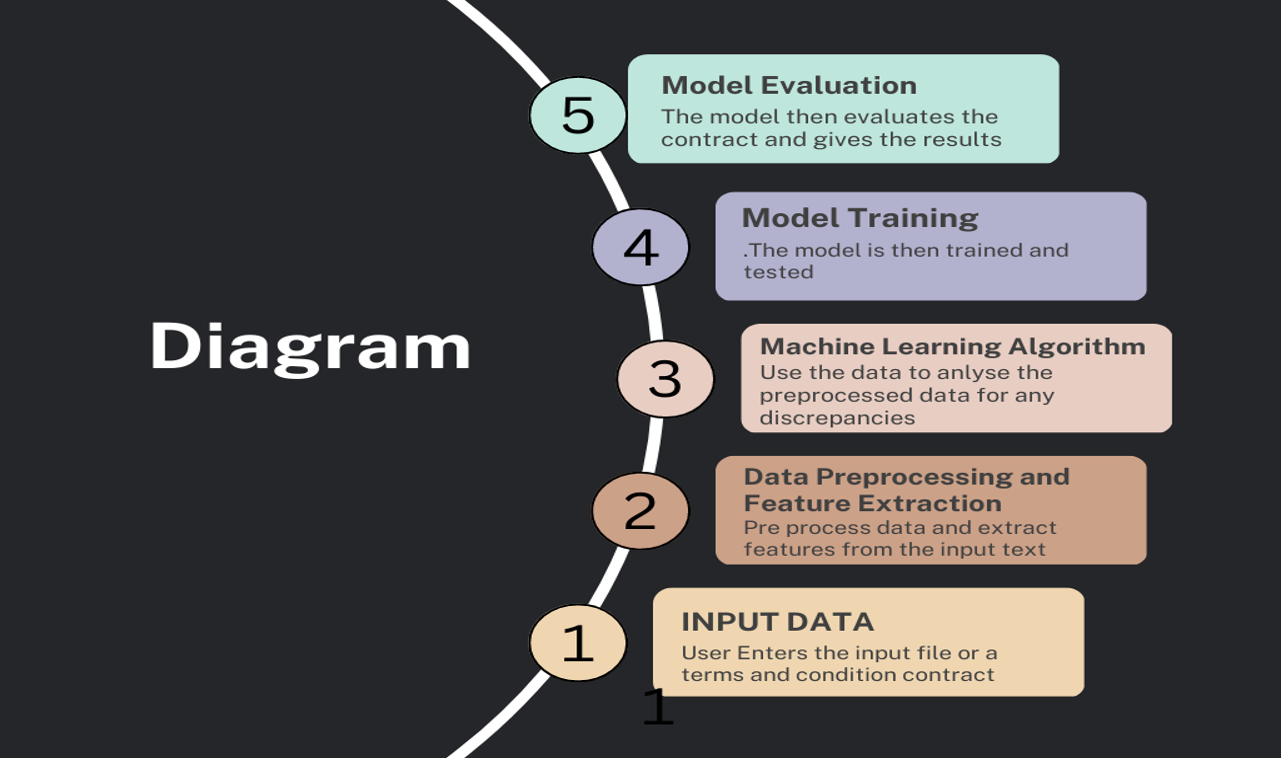
\includegraphics{Figures/Diagramoftheproposedsystem.png}}
\caption{\label{Figure::Diagram Of The Proposed System} Diagram Of The Proposed System  \ref{Figure::Diagram Of The Proposed System}}
\end{figure}





\newpage

\section{Mission Statement \label{Section::Mission Statement} }
The primary purpose of this project is to protect stakeholders from falling victim to deceptive clauses in contracts that may undermine their best interests, either intentionally or unintentionally or via other disruptive means. These clauses could cause harm to the signing party through various means, such as monetary loss or other negative consequences that may impact the livelihood of the concerned stakeholder as a whole. 
The proposed machine learning software system aims to detect and flag such fraudulent clauses in terms and conditions contracts, thus empowering stakeholders to make informed decisions before committing to an agreement. 
By leveraging advanced machine learning algorithms, the system will analyze and identify potential risks in the contract language. This approach ensures that stakeholders are aware of any hidden or obscure terms that could be detrimental to their interests. In addition to enhancing the transparency of contractual agreements upheld in a court of law, the software will enable users to negotiate better terms, minimize potential disputes, and ultimately establish a more secure and trustworthy contractual environment.
\chapter{Scope \\
%\small{\textit{-- Team-11}} 
\index{Chapter!Scope}
\index{Scope}
\label{Chapter::Scope}}



\section{Identification\label{Section::Project Identification} }


\section { Document Overview \label{Section::Document Overview} }



\section{System Overview\label{Section::System Overview}}
% The primary goal of this project is to develop a machine learning model that assists stakeholders in avoiding deception by clauses in terms and conditions (T\&C ) contracts. This approach will automatically analyze all clauses within the contract, providing stakeholders with the necessary information to decide whether to proceed or not.
% Several popular machine learning libraries, such as scikit-learn \cite{scikit-learn}, the Natural Language Toolkit (NLTK) \cite{nltk}, and Keras \cite{keras}, will be utilized to create the model. Flask \cite{flask} and Django \cite{django} will be employed to develop the web application, enabling users to upload T\&C contracts in text or PDF formats and evaluate the presence of any deceptive clauses. Scikit-learn, NLTK, and Keras are widely used libraries for machine learning tasks.
% We will start by selecting a dataset of T\&C contracts that have been identified as containing fraudulent or unclear clauses. The scikit-learn and Keras libraries will be used for feature extraction, where we can extract relevant information from the text. After extracting the features, we can use them to train a machine learning AI model using the scikit-learn engine.
% Once the AI model is trained, it can be evaluated using the Keras library to determine its accuracy. If the model performs well, it can be used to identify whether clauses in T\&C contracts are fraudulent or unclear.
% In summary, this project aims to create a machine learning model that helps stakeholders avoid deception in T\&C contracts by automatically analyzing the clauses within the contract. By using popular libraries and web development frameworks, the model will provide stakeholders with valuable insights and help them make informed decisions about whether to proceed with an agreement or not.

% \begin{figure}
% \centering
% \scalebox{0.53}{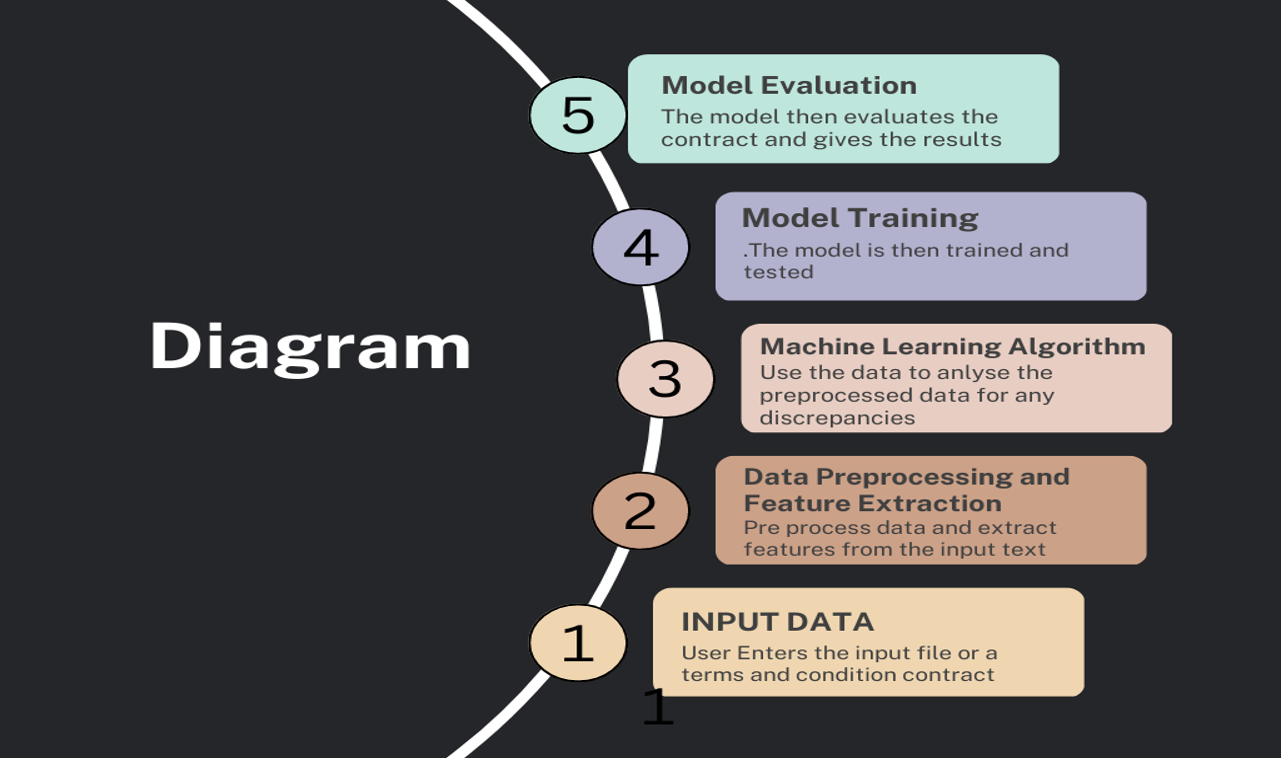
\includegraphics{Figures/Diagramoftheproposedsystem.png}}
% \caption{\label{Figure::Diagram Of The Proposed System} Diagram Of The Proposed System  \ref{Figure::Diagram Of The Proposed System}}
% \end{figure}

\chapter{Referenced Documents \\
%\small{\textit{-- Team-11}} 
\index{Chapter!References}
\index{References}
\label{Chapter::References}}

\begin{itemize}
    \item IEEE Std 1362-1998, IEEE Guide for Information Technology—System Definition—Concept of Operations (ConOps) Document, Approved March 19, 1998.

    \item Dr. Muresan, David Darian. Lecture-5, Lecture-05-Concept Of Operations( ConOps), Stevens Institute Of Technology, 2023
    \item Dr. Muresan, David Darian. Lecture-10, Lecture-10-Requirements Analysis, Stevens Institute Of Technology, 2023
    \item Dr. Muresan, David Darian. Lecture-2, Lecture-2-Stakeholders, Stevens Institute Of Technology, 2023
    \item Dr. Muresan, David Darian. Lecture-3, Lecture-3-Business Requirements, Stevens Institute Of Technology, 2023
    \item Dr. Muresan, David Darian. Lecture-4, Lecture-4-User Requirements, Stevens Institute Of Technology, 2023
    \item Dr. Muresan, David Darian. Lecture-6, Lecture-6- Requirements Elicitation, Stevens Institute Of Technology, 2023
    

    
\end{itemize}
\chapter{Current System Or Situation \\
%\small{\textit{-- Team-11}} 
\index{Chapter!Current System Or Situation }
\index{Scope}
\label{Chapter::Current System Or Situation}}
The motivation behind developing this system is that currently, stakeholders, which in this case would be common person, without much knowledge about the law, are required to manually read through terms and conditions contracts which can often be super long, time consuming and notoriously confusing due to the amount and complexity of the legal terms used, that are at the end of the day, accepted in a court of law, which would be unfamiliar to a common person thereby, risking themselves of inflicting harm in a shape that may result in financial, personal or mental distress. While the option to consult a lawyer exists, it is not always feasible due to their high costs and availability constraints.

In the absence of an effective tool to navigate this challenging problem, the need for a solution like ClauseGuard became apparent. This system is designed to safeguard stakeholders from potential pitfalls hidden in deceptive clauses. By providing a machine learning-based analysis of contracts, ClauseGuard offers a reliable, user-friendly, and cost-effective alternative to traditional methods of consulting a lawyer, fostering a safer and more transparent contract review process.  

\section{Background, objectives, and scope \label{Section::Background,objectives and scope} }
The current system exists to ensure that stakeholders, typically common individuals, are equipped to agree to the terms and conditions contracts set forth by the initiating party. This process, however, is often lengthy, complex, time-consuming, and challenging for the average person to fully understand the implications of the contract. While professional consultation is an option, the high costs associated with it often render it an unfeasible choice.

The mission of the proposed system, Clauseguard, is to ensure that stakeholders can effectively parse through the terms and conditions contract presented by the initiating party. The ultimate aim is to make stakeholders aware of any deceptive or harmful clauses in the contract, thereby safeguarding them from potential financial, personal, or other forms of harm.
 The scope of the proposed system extends to stakeholders from any background ranging from a common person to a lawyer, govermental agencies and mega corporations who may encounter contractual agreements. The objective is to provide support and enhance their understanding of the contracts they engage with, regardless of the complexity of the legal language involved. 



% The primary purpose of this project is to protect stakeholders from falling victim to deceptive clauses in contracts that may undermine their best interests, either intentionally or unintentionally or via other disruptive means. These clauses could cause harm to the signing party through various means, such as monetary loss or other negative consequences that may impact the livelihood of the concerned stakeholder as a whole. The proposed machine learning software system aims to detect and flag such fraudulent clauses in terms and conditions contracts, thus empowering stakeholders to make informed decisions before committing to an agreement.

% By leveraging advanced machine learning algorithms, the system will analyze and identify potential risks in the contract language. This approach ensures that stakeholders are aware of any hidden or obscure terms that could be detrimental to their interests. In addition to enhancing the transparency of contractual agreements upheld in a court of law, the software will enable users to negotiate better terms, minimize potential disputes, and ultimately establish a more secure and trustworthy contractual environment.

\section { Operational policies and constraints \label{Section::Operational Policies and constraints}}
There are a number of operational policies and constraints that are applied to the proposed system.
\subsection{Operational Policies}
An operational policy can be defined as a general statement of required behaviour. The operational policy of clauseguard is as follows: 
\begin{itemize}
    \item Data privacy is a major cause of concern for the proposed system. Sensitive and confidential information would be shared on an open internet website. As such, the system must ensure that no information is stored on any backend servers in the form of "cookies", "tokens" or any similar data logging services. The system should respect data privacy laws partaining to each individual country and follow guidelines as set forth by that particular country. 
    
    \item The system must explicitly ask stakeholders for their consent for analyzing the submitted documents before using the system. This consent would be devised by a team of professional experts and lawyers so as to not hold the parent organization of clauseguard of any legal ramifications. 

    \item The system must utilize a sophisticated machine learning algorithm that is retrained and updated at intervals of every two months. This ensures that the model stays current with the evolving nature of legal language in contracts, reflecting the latest laws and regulations. Additionally, cross-checking with historical legal data is done during these updates to maintain consistency and accuracy. Periodic reviews by legal experts complement the machine learning model, ensuring its recommendations remain accurate and legally sound.

    \item the system must provide clear explanations for any detected clauses in the Terms & Conditions contracts. These explanations are devised by the system based on the analysis of datasets comprising other legal documents of similar nature and scope. This ensures that users not only receive information about potential issues in the contracts they're reviewing, but also gain an understanding of why these clauses may be problematic.
\end{itemize}

\subsection{Operational Constraints}
An operational constraint is an externally imposed condition that must be observed. The operational constraint of clauseguard is as follows: 
\begin{itemize}
    \item The machine learning algrothim would require extreme amounts of processing power and computational resources, which, on failing to secure, would severely limit the number of contracts that can be analyzed. It can also lead to network wide crashes and instability. 
    \item The model depends on the accuracy of the dataset on which it is trained. Lack of available legal documents can induce severe challenge on the authenticity and accuracy of the model. Some countries do not disclose legal documents into the public domain, thereby severely limiting the use of this model in certain geographic locations. 
    \item The model must be online 24/7 365 days of the week. Lack of server resources can cause an availability constraint. 
    \item The model must comply with data regulations  and privacy laws around the world. This constraint cannot be guranteed across every country, as each country has extremely wide definations of data privacy laws, failing to adhere can cause a ban of this sytem in that particular country. 
    \item The model must handle contracts written in different terminologies and structures used across various different countries. For example, Japanese legal system requires legal documents to start from the right to left. Training the model on many different structures is a significant operational constraint. 
    \item The model must ensure the security of private and sensitive data. This is also a major operational constraint as unethical hacking can lead to significant data leaks. 
    
\end{itemize}

\section{Description of the current system or situation \label{Section::Description of the current system or situation}}
The current system is being built with the primary objective of developing a machine learning model to aid stakeholders in identifying potentially deceptive clauses in terms and conditions (T\&C) contracts. This system functions by automatically scrutinizing all clauses within the contract, thereby equipping stakeholders with crucial information needed to make an informed decision regarding their agreement to the terms.
The system uses several machine learning libraries such as scikit-learn, natural language toolkit(NLTK) and keras for the creation of the model. 

Scikit-learn is a machine learning library in Python that provides tools for data analysis and modeling. In this system, scikit-learn is primarily used for preprocessing the dataset and training the machine learning model. It provides utilities for common machine learning tasks such as feature extraction, text representation, and model evaluation. For instance, scikit-learn's text feature extraction utilities can convert the text data in T&C contracts into a format that can be input to the machine learning model.
Natural Language Toolkit (NLTK) is a library in Python that provides tools for working with human language data (text).  In this system, NLTK is primarily used for tokenization (i.e. breaking up of sentences into each indidual alphabet, white space, special character, symbol etc), stemming (A process to remove the suffix from words such as ing), and lemmatization (converting the word into its root form and reducing the superlative of the word into its equivalent comparative, for example: oldest will be old), which are crucial steps in preprocessing the text data.

Keras is a high-level neural networks API in Python.  
It is used to define and train any kind of deep learning model. In this system, Keras is used to define the machine learning model structure and train the model using the preprocessed dataset.

Flask and Django are web development frameworks in Python.  In this system, Flask and Django are used to build the web application that allows users to upload T&C contracts and get the results from the machine learning model. Flask can handle simpler and smaller loads, while Django can manage more complex and larger loads. The choice between them would depend on the requirements and scalability plans of the system. Flask would be used for the inital build of the system followed by django for a more advanced model. 

The system operates by facilitating users to upload a T&C contract via a web interface, developed using Flask or Django. The uploaded contract undergoes a preprocessing step, where it's transformed into a suitable format for the machine learning model using libraries such as scikit-learn and NLTK.

The preprocessed data is then fed into a machine learning model, constructed and trained using the Keras library. This model evaluates each clause in the contract, assigning a risk score that represents the likelihood of the clause being deceptive or unfair.

The output provided to the user includes highlighted sections of the contract that have been flagged as potentially deceptive, along with a percentage indicator that quantifies the overall risk associated with the contract. For each highlighted section, the system also provides an explanation, derived from the model's analysis, clarifying why the clause was flagged.

With this information, the user is empowered to make an informed decision about whether to sign the contract or not. 
The breakdown of the system is as follows: 
\begin{itemize}
    \item Operational Environment and its characteristics: The current environemtn invloves stakeholders using a web platform to upload their T\&C contract into a web interface. 
    \item Major system components and the interconnection among those components: The system comprieses of a machine learning model that is trained on a vast amount of datasets invlovling legal documents from various bracnches of the law such as crimaal law, corporate law, copyright protect, patent law, etc. The model parses each line in the contract, signals out protential harmful clauses that may seek to cause harm to the signing party in the shape of montery or mental duress, and quantifies the risk carried with the contract signified by a percentage. Furthermore, the model genewrates expplainations for the harmful clauses it has highlighted. 
    \item Interfaces to external systems or procedures: The system can be accessed on any platform, device and operating systems. Similar to chatgpt, an api for the model will be released whcih can be integrated into propirety systems that are otherwise not avaialbe to the general public and are the intellectual property of their respective owenrs. 
    \item Capabilities, functions, and features of the current system: The system's objective is to analayze and interpret complicated legal terms, identifying potentially harmful clauses and providing layman explainations to the user. The system's function includes parsing throug each line of the document, running the parsed text through the machine learning model and generating a small report accessable within the website itself that includes a risk assessment percentage as well as a succint explaination, 
    \item e)                \begin{figure}[H]
    \centering
    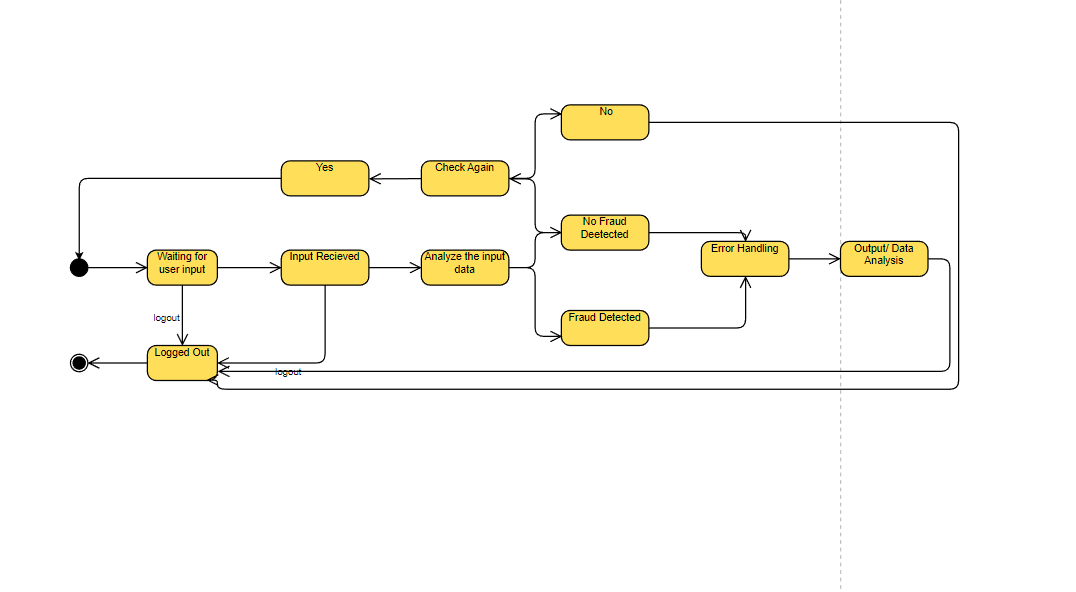
\includegraphics[scale=0.83]{Figures/state machine.png}
    \caption{State Machine View of the diagram \ref{fig:state machine}}
    \label{fig:state machine}
\end{figure}
   

    \item Cost of system operations: The cost of running the system would depend upon the amount of resources that it would take to run the model on servers accessible throughout the world wide web whist analyzing millions of documents concurrently. Load balancers and other such infrastructure must be set up to ensure the working for the model. Infrastructure like the Amazon AWS could be used to set up the model. This would solve the problem with data protection too.  Maintenance would require additional funds. Overall, a cost in the 7 figure range is expected for the initial version of the system 

    \item Operational risk factors: Several operation risk factors could occur which include inaccurate intepretation and explaination, legal reprucssions, confidential Data leaks, Security breaches, server crashes, instability, low accuracy, inaccurate percentages and so on. 
    \item Performance characteristics: The model should be fast, accurate and able to process large quantities of data. To ensure these non-functioanl requirements, the model can be set up on additional infrasture such as could bases services. Amazon AWS would benefit the model tremedously. 
    \item Quality attributes: The model should aim for high availability, reliability and secuity. Becuase of the nature of deleaing with legality of a country, accuracy, avaialbity and reliability are of utomost importance. 
    \item Provisions for safety, security: Due to the nature of the model itself, sensitive and confidential data will be shared. The model must ensure data privacy and secuity of the system to prevent potential breaches and subsequent leaks of confidential data. The system must be designed to ensure high frequency of backed up data to guarantee swift recovery of said data if  operational failures occur. 
\end{itemize}

 



\section{Modes of operation for the current system or situation \label{Section::Modes of Operation for the current system or situation}}
The system will operate on various modes of operation throughout its lifecycle as detailed below: 
\begin{itemize}
    \item Training Mode: This mode is only accessible to the system's developers and not to the end users. It plays a crucial role in the functioning of the system as this is where new features are developed, the model is trained on additional datasets, and existing defects are patched. The training mode uses large amounts of T\&C contracts to train the machine learning model to understand the structure, language, and meaning of various clauses. This process allows the model to learn how to distinguish between benign and deceptive clauses. Enhancements and updates to the system are made in this mode before being deployed to the Operational Mode. 
    \item Operational Mode: This model is the primary end product of the system used by the users to upload T\&C contracts for analysis. The system would use the model developed in the training mode to evaluate the uploaded contract. It identifies potentially deceptive clauses, calculates the overall risk associated with the contract, and provides explanations for flagged sections. The results are then displayed to the user, who can use this information to make an informed decision about whether to sign the contract.
    \item Emergency Mode: This mode serves as a contingency plan, activated in the event that both the Primary and Training modes experience operational failures. The Emergency Mode relies on a legacy version of the currently deployed primary model. This fallback mechanism ensures continuity of service even in the face of unforeseen disruptions. While it may not have the most recent updates and features available in the Primary Mode, the Emergency Mode is designed to effectively analyze T&C contracts and identify deceptive clauses, thereby maintaining the core functionality of the system. Regular checks and minor updates are carried out to ensure that the Emergency Mode is always ready for activation, should the need arise. This robust backup plan contributes to the system's resilience and reliability, offering users a dependable tool for contract analysis at all times.
    


\end{itemize}


\section{User classes and other involved personnel \label{Section::User Classes and other involved personnel}}
Clauseguard would involve the participation several user classes and  personal either directly or indirectly depending upon their interaction with the system as given below: 
\begin{itemize}
    \item End User: The end users are the primary users of clauseguard. They interact directly with the system by uploading the T\&C contracts for analysis. Their interaction is via the web platform, with the aim of identifying deceptive contracts in T\&C contracts. They don't require any skill levels except basic computer skills. 
    \item Developers: They are the primary coders of the system. Their responsibilities include, implementing new features, functionality and maintenance of the system. They require high skill levels in the fields of programming and problem-solving as they require a high level of technical skill and familiarity with the underlying technology.
    \item Machine Learning Specialists: ML specialists work to continually improve clauseguard's machine learning algorithm. They are responsible for training the model on new datasets, testing performance and implementing updates as needed. Their interaction is through machine learning libraries used in the development of the model. 
    \item CyberSecurity Experts: These individuals play a crucial role in safeguarding the ClauseGuard system from unauthorized access and potential security threats and are arguably the most important stakeholders in the functioning of clauseguard as a service. They are tasked with the responsibility of thwarting attempts by unethical entities, often referred to as hackers, who might attempt to breach the system and gain access to confidential data. Cybersecurity experts work diligently to identify and secure any potential vulnerabilities in the system that could be exploited for malicious purposes. Their interaction with the system spans across all areas, but they primarily focus on the system's edge cases and potential weak points that could be susceptible to breaches. They are proficient in the latest cybersecurity protocols and techniques and utilize this expertise to constantly enhance the system's security measures. In addition, they collaborate closely with the system administrators and developers to ensure that security is integrated into all aspects of the ClauseGuard system, from the web application to the machine learning model itself. Their work helps maintain the trust of the end-users by ensuring that their interactions with the system remain secure and confidential.
    \item Legal Consultants: Although their involvement may not be direct, they nevertheless, play a crucial role in the development of the model. They review the machine learning model's output to ensure its accuracy and make recommendations for improvement based on their legal expertise. They interact indirectly with the system by providing feedback and suggestions for model enhancements based on their understanding of legal terminologies and concepts.
    \item Commercial enterprises stand to gain significantly from the use of the ClauseGuard system. These entities often engage in complex transactions that involve extensive legal contracts. With the help of ClauseGuard, they can quickly and efficiently review these contracts, expediting the deal-making process. For instance,  the  purchase of Activision-Blizzard by Microsoft made headlines across the tech industry. In such scenarios, missing or overlooking crucial legal details can lead to considerable impediments, potentially blocking the deal altogether which happened in the case of Microsoft acquiring Activision-Blizzard. ClauseGuard can mitigate such risks by identifying potentially harmful or unclear clauses that could jeopardize the agreement. This can save enterprises substantial time and resources, while also providing them with a layer of protection against contractual pitfalls. Similar to end users, commercial enterprises need only basic computing skills to access clauseguard. 

\end{itemize}


\section{Support environment \label{Section::Support Environment}}
Clauseguard will have a number of support systems in place that will fortify the absolute working of the system to its fullest capacity. 
\begin{itemize}
    \item Clauseguard will have a dedicated technical support team. This team will handle technical queries, troubleshoot reported issues and work on continuous improvement of the system. 
    \item Since clauseguard would primarily be virtual, the equipment and facilities would involve robust server architecture preferbly on cloud bases services such as AWS, load balancers for handling multiple connection requests and IT infrastructure for the support team to handle issues effectively. 
    \item Clauseguard would have a customer service team and infrastructure to manage user inquiries, issues and feedbacks. This platform would involve efficient tracking and resolution of support tickets. 
    \item ClauseGuard , being a cloud-based application, would use secure cloud storage services to store user data and application elements essential for the functioning of the system. It is to be noted that any personal or confidential data will not be stored in any capacity. 
\end{itemize}





\chapter{Justification for and nature of changes \\
%\small{\textit{-- Team-11}} 
\index{Chapter!Justification for and nature of changes }
\index{Justification for and nature of changes}
\label{Chapter::Justification for and nature of changes}}\



\section{Justification of changes  \label{Section::Justification of changes} }
Justification for the changes of the proposed systems is outlined below: 
\begin{itemize}
    \item New or modified aspects: The rapidly changing legal landscape and increasing complexity and ambuity in T\&C contracts propelled the need for an efficent and reliable system that can adapt and and update itself based on the latest laws and guidelines. 
    \item Limitations of the current systems: At the moment, most contracts are manually reviewed by legal professionsals. This process is time0consuming, tedious and prone to error. Furthermore, the interpretation of different terms and conditions may vary between different individuals leading to inconsistancies in evaluations. 

    \subsection{Justification for a new or modified system}
    Clauseguard can effectively counter the challenges faced by the current system as outlined below: 
    \begin{itemize}
        \item With the advent of the COVID-19 pandemic, there has been a significant uptick in the usage of digital contracts. This transition has led to a surge in data volumes that traditional methods of review cannot efficiently handle. ClauseGuard's machine learning model, with its inherent ability to process and analyze vast amounts of data swiftly and accurately, stands to offer an invaluable service in this context. It can help stakeholders navigate through the labyrinth of digital contracts, ensuring they are informed and protected. This capability is not just a convenience; it is a necessity in the rapidly digitizing world, where the velocity and volume of contractual agreements are ever-increasing. 
        \item The machine learning system aims to automate the evaluation of contracts, significantly reducing the time and resources required, thereby leading to lower operational costs. It can also improve consistency in evaluations by reducing subjective human interpretation.
        \item The capability to autonomously detect deceptive or unclear clauses within contracts has become increasingly necessary in today's rapidly evolving legal landscape. Contracts are becoming more intricate and are subject to frequent revisions due to changing regulations and business practices. These complexities often make it challenging for individuals to fully comprehend the terms, leading to potential misinterpretations and unintended commitments. An automated system that can reliably dissect and interpret these complexities not only promotes transparency but also serves as a protective measure for stakeholders. 
    \end{itemize}
    
\end{itemize}


\section{Description of desired changes \label{Section::Description of desired changes}}
Clauseguard has a number of capabilites, interfaces and personel changes which are highlighted below: 

\begin{itemize}
    \item Capability Changes: The implementation of the machine learning model will introduce new capabilities such as automated analysis of T&C contracts, detection of deceptive or unclear clauses, and explanations for detected clauses. While the original system relied on manual inspection and comprehension of contract clauses, the new system will automate this process, significantly reducing the time and effort required to review contracts. Moreover, it would be cost effective for those individuals who otherwise, would not abe able to affort professional legal opinion.
    \item System Processing Changes: The machine learning model process the uploaded contracts, analyze the clauses, and output results indicating the presence of any deceptive clauses along with explanations for the same. 
    \item  Interface Changes: The user interface will be modified to allow users to upload contracts and view results. This interface will need to be intuitive and user-friendly, providing clear instructions on how to upload contracts and view results. Changes to the interface will also need to accommodate the presentation of results, which will now include highlighted clauses and their explanations.
    \item Personnel Changes: The development and maintenance of the machine learning model will require personnel with expertise in machine learning, natural language processing, and contract law. Additionally, user training may be required to educate users on how to interact with the new system and interpret its outputs.
    \item Personnel Changes: The development and maintenance of the machine learning model will require personnel with expertise in machine learning, natural language processing, and contract law. Additionally, user training may be required to educate users on how to interact with the new system and interpret its outputs.
    \item Environment Changes: The implementation of the machine learning model will digitize the contract review process, requiring an operational environment that can support the deployment and use of this technology. This may involve changes to existing IT infrastructure and the adoption of new technologies to support the model.
    \item Operational Changes: The introduction of the machine learning model will fundamentally change how contracts are reviewed traditionally. Instead of manually reading through contracts, users will upload them to the system for analysis. This will change the operational procedures and daily work routines of the users.
    \item Support Changes: The implementation of the machine learning model will necessitate changes in the support requirements. Technical support will need to be available to address any issues that arise with the use of the machine learning model. Moreover, regular updates and maintenance will be required to ensure the model remains up-to-date with changes in contract law.
    \item Other Changes: As a result of the implementation of the machine learning model, there may be changes to the time required to review contracts. As the process becomes more automated, it is likely that contract review times will be significantly reduced, allowing for quicker decision-making, faster legal processes and reduction in the cost of paralegal teams. 














\end{itemize}


\section{Priorities among changes \label{Section::Priorities among changes}}
The proorites for the system ClauseGuard are highlighted below: 
\begin{itemize}
    \item Essential Features: \begin{itemize}
        \item The core feature of the system is its ability to identify and highlight potentially fraudulent clauses within a contract. Without this feature, the system would not serve its primary purpose. Failure to implement this would lead to users not being able to identify potential risks in contracts.
        \item The system should be able to assign a risk percentage to each contract, indicating the level of potential fraud. This is vital as it quantifies the risk involved, aiding users in their decision-making process.


        \item Each identified risk should come with an explanation to help users understand the reasons why the clause has been flagged as fraudulent. Without this feature, users may be left confused about the nature of the risk involved.


       
        




    \end{itemize} 

    \item Desirable Features: 
    \begin{itemize}
        \item While not essential, having an intuitive and easy-to-use interface would greatly enhance user experience, encouraging more frequent use and increasing user satisfaction.

        \item The ability to integrate with common document management systems would make the application more versatile and convenient to use. It would allow users to directly upload contracts for analysis from a wide range of document format systems.

        \item  An ability to analyze and present a comparison of risk percentages. This feature would provide users with an onjective metric along with an explaination of why that specific clause was highlighted intended to allow the user to make an informed decision. The decision, ultimately, is left upto the descretion of the user. 

    \end{itemize}

    \item Optional Features: 
    \begin{itemize}
        \item The ability to process and analyze contracts in multiple languages would increase the usability of the system across different geographic locations and allow for greater control over the scanned documents.
        \item A feature that allows multiple users to view and discuss the same contract in real-time. This can facilitate faster decision-making, especially in larger teams similar to that of what the platform "Overleaf" does for LaTeX documents.
        \item Providing API access would allow third-party developers to integrate ClauseGuard's features into their own applications.
        \item Allowing users to directly sign off on safe contracts via popular e-signature platforms could streamline the contract approval process such as adobe signature. 
        \item A feature that allows users to customize the risk percentage threshold that triggers a flag, enabling a more personalized user experience.
        \item  feature that tracks and displays changes made to a contract over time, helping users see how the risk assessment has evolved.

    \end{itemize}

\end{itemize}




\section{Changes considered but not included \label{Section::Changes considered but not included}}
Some features that were considered for ClauseGuard but were not included as follows: 
\begin{itemize}
    \item A Real-Time Fraud Detection feature would have allowed the system to analyze contracts and detect fraudulent clauses as the user is typing or editing the contract. However, due to the significant computational resources required for real-time analysis and the potential disruption to the user experience due to lag or delay, this feature was not included.
    \item A feature for automatic contract modification which would allow the system to suggest modifications to contracts to eliminate or mitigate the risk of identified fraudulent clauses. However, this was not included due to the potential legal implications and the complexity of accurately generating legally sound contract language.
    \item An AI chatbot feature was considered to provide immediate assistance to users. However, due to the complexity of developing a chatbot that can accurately understand and respond to a wide range of user queries, this feature was not included.




\end{itemize}
Note: Although the above features are not included at this time of development, these are features that could be looked at to add on at a later stage of ClauseGuard's life cycle. 

\section{ Assumptions and Constraints \label{Section::Assumptions and Constraints}}
The assumtions and constraints of clauseguard are as follows:
\begin{itemize}
    \item Assumptions: An assumption is defined as a condition that is taken to be true. Some of the assumptions for ClauseGuard are: 
    \begin{itemize}
        \item Data Availability: We assume that the system will have access to a sufficient number of sample contracts with and without fraudulent clauses for training the machine learning model.
        \item User Literacy: We assume that users have a basic understanding of contractual language and terms, as this will influence how they interact with the system and interpret the risk assessments.
        \item Scalability: We assume that the number of contracts to be analyzed will increase over time as more users adopt the system, necessitating a scalable architecture.
        \item Legal Compliance: We assume that all analyzed contracts will be in compliance with local laws and regulations, which the system will need to be updated to reflect.






    \end{itemize}
    \item Constraints: A constraint can be defined as an externally imposed limitation placed on the new or modified system or the processes used to develop
or modify the system. Some of the constraints of ClauseGuard are as follows: 
\begin{itemize}
    \item Budgetary Constraints: The development and maintenance of the system is subject to the availability of funds. This might limit the number of features that can be implemented at a given time.
    \item Time Constraints: The system must be developed and made operational within a specified timeframe. This could limit the amount of testing and refinement that can be done before launch.
    \item Privacy Constraints: The system must comply with data privacy laws and regulations, such as GDPR. This could limit the type of data that can be collected and how it can be used. The system must also take into account some countires that are cut off from the rest of the world such as Russia, Azerbaijan, Kyrgyzstan etc. 


\end{itemize}
\end{itemize}


\chapter{Concepts for the proposed system \\
%\small{\textit{-- Team-11}} 
\index{Chapter!Concepts for the proposed systems }
\index{Concepts for the proposed system}
\label{Chapter::Concepts for the proposed system}}\



\section{Background, objectives, and scope \label{Section::Background,objectives,and scope proposed}}
The rationale for the proposed approach is that it can be challenging for people to spot fraudulent elements in contracts since they are sometimes buried within lengthy and complicated terms and conditions. The suggested system's goal is to identify dishonest clauses in contracts using machine learning techniques, which will increase the contracts' fairness and transparency for all parties. The proposed system's scope includes contract analysis across a range of industries, including technology, insurance, and financial services.


\section{Operational policies and constraints \label{Section::Operational Policies and Constraints proposed}}
The system must make sure that user data is not abused or disclosed without permission, and that the data it gathers and analyzes is handled securely and confidentially.
The system must be precise and trustworthy in spotting contract fraud. The algorithms and outcomes of the system must be rigorously tested and validated for this.


\section{Description of the proposed system \label{Section::Description of the proposed System proposed}}
To find potentially dishonest clauses in contracts, the suggested method will employ machine learning algorithms and natural language processing. Contracts will be analyzed by the system, and any clauses that seem to be unfair, misleading, or deceptive will be flagged. The system will also explain its findings so that consumers may comprehend the justification for the system's choices.



\section{Modes of operation \label{Section::Modes of operation proposed}}

The suggested system will function in two different ways:

In manual mode, a user can upload a contract to the system for analysis, and the system will then give that analysis.

Real-time mode, when the system continuously checks contracts for dishonest clauses and alerts the user to any potential problems.


\section{User classes and other involved personnel \label{Section::User Classes and other involved personnel proposed}}
People and organizations involved in contract formulation and approval will make use of the suggested system. These professionals working with contracts include attorneys, contract managers, compliance officers, and others. Additionally, the system will work with specialists in machine learning who will be in charge of enhancing and refining the system's algorithms.


\section{Support environment \label{Section::Support Environment proposed}}
User guides, online help, and a customer service team will all be part of the support system for the planned system. The system will also include a feedback tool that will let users comment on how well the system is working and recommend changes. To guarantee that the system is operating at its peak performance, routine upgrades and maintenance will be offered.



\chapter{Operational scenarios 
%\small{\textit{-- Team-11}} 
\index{Chapter!Operational scenarios }
\index{Operational scenarios}
\label{Chapter::Operational scenarios}}\

A scenario can be defined as a  step-by-step description of how the proposed system should operate and interact with its users and its
external interfaces under a given set of circumstances. The operational scenario for the following proposed system is outlined below
\begin{itemize}
    \item Normal Operation Scenario: The user navigates to the website, facilitated by a user-friendly interface designed for ease of use. They are greeted by clear instructions and prompts guiding them to upload a Terms and Conditions (T\&C) contract. This can be in various formats such as text, PDF, or LaTeX document, providing ample flexibility to the user.

Once the contract is uploaded, the system initiates the preprocessing stage. This involves cleaning and formatting the text data, utilizing Natural Language Processing techniques such as tokenization, stemming, and lemmatization. This step ensures that the machine learning model receives the data in a suitable format for analysis.

Upon completion of the preprocessing stage, the data is fed into the machine learning model, which has been trained on a vast dataset of T\&C contracts. The model thoroughly scrutinizes the clauses in the contract, identifying any potential deceptive or unclear clauses.

The user then receives a comprehensive report, detailing the analysis results. The report includes a percentage counter indicating the proportion of potentially deceptive clauses found in the contract. Each flagged clause is highlighted, and clicking on it provides a brief explanation as to why it was flagged by the model.

With this detailed insight, the user is better equipped to make an informed decision on whether to proceed with the contract. To proceed with the contract, is left upto the discretion of the user. 

\item Stress handling scenario: A stress handling scenario occurs in a situation where multiple users simultaneously access the website, potentially leading to the analysis of millions of documents concurrently. In such high-demand situations, the system is designed to maintain operational efficiency, ensuring that all users receive a timely and accurate analysis of their contracts.

To manage this high traffic, the system utilizes a sophisticated load balancing mechanism. This mechanism dynamically allocates system resources to different tasks based on demand, ensuring that no single task is overburdened. The load balancer distributes the workload across various system servers located on strategic geographic locations, preventing any bottlenecks or system slowdowns.

Furthermore, the system is built with scalability in mind. It has the capacity to ramp up resources when demand surges, such as during peak usage hours. This ensures that even in times of heavy load, the system remains responsive and continues to deliver results promptly.

Lastly, the system employs robust error handling techniques. In the rare event of a failure or error, the system is designed to recover gracefully, minimizing the impact on the user. Alerts are sent to the system administrators to ensure rapid response and resolution.

Through these measures, the system can effectively manage stress scenarios, providing reliable, efficient service to all users, even during periods of peak demand.

    \item Error handling Scenario: An error handling scenario comes into play when a user attempts to upload a contract in an unsupported file format. In such a situation, the system is designed to promptly identify the issue and respond appropriately and in a timely manner.

Upon detecting an unsupported file format, the system triggers an error message. The system informs the user that the uploaded contract file format isn't supported and kindly prompts them to upload the contract again in a compatible format.

In addition, this error message includes a list of the supported file formats for the user's convenience. This  approach not only resolves the issue at hand but also educates the user about the correct file formats, preventing the same error from reoccurring in the future.

Furthermore, the system logs this error in a database. These logs are periodically reviewed by the system administrators to identify patterns and potential areas for system improvement. For instance, if a particular unsupported file format is frequently attempted by users, the team may consider adding support for that format in future system updates.

Thus the error handling scenario is designed to be user-centric in its approach and its commitment to provide a seamless, intuitive user experience. 

 \item Degraded Operation Scenario: A system degradation scenario comes into play when there's an unforeseen failure with the primary system. In such instances, our robust backup strategy ensures that service continuity is maintained, albeit the service may not be as robust as the primary model.

Upon detection of a primary system failure, the system automatically transitions to a legacy version. This redundancy plan allows users to continue accessing the system and uploading contracts for analysis, ensuring that the primary functionality of the system. remains available. This would also ensure that there is no monetary loss to the organization in the event of a catastrophic system failure. 

However, its important to note that while the legacy system is fully functional, it might not match the performance, accuracy, or feature set of the primary system. As it is an older version, it may process contracts more slowly, and its clause analysis might not reflect the most recent legal developments or algorithmic improvements.

During this degraded mode operation, users will be informed about the temporary switch to the legacy system via a notification on the website. This message reassures them that services are still operational, but also sets appropriate expectations about the temporary limitations they might experience.

Meanwhile, our dedicated team of technicians would be alerted to the issue and would begin troubleshooting the primary system. The goal would be to restore the primary system to full functionality as quickly as possible to minimize the time users spend operating under the degraded mode.

This degradation scenario works towards highlighting our commitment to service reliability and continuity. We understand that our users depend on our system, and we have contingency plans in place to ensure that unexpected issues don't interrupt the availability of our services.

    \item Emergency scenario: In the event of a security breach, our system swiftly transitions to a minimally functioning mode to prioritize data protection and system integrity.

Upon detecting a potential security threat, our system automatically triggers its emergency protocol. This protocol includes limiting user access, suspending non-essential operations, and activating enhanced security measures. The aim is to isolate the breach, protect sensitive data, and prevent further unauthorized access to ensure no confidential or sensitive data is leaked.

During this emergency mode, users may encounter restricted functionality. Access to majority of the services might be temporarily suspended , and the overall system performance may be reduced. However, these measures are critical to maintaining the security of the system and safeguarding user's data.

Simultaneously, our cybersecurity team would be alerted to the situation. These experts would immediately initiate an investigation into the breach, working tirelessly to neutralize the threat and restore the system to full functionality. Users would be notified about the situation and would be kept informed about progress towards resolution.

This emergency scenario highlights our commitment to data security and system integrity. We understand the critical importance of protecting sensitive information, and our system is designed to respond effectively to any security threats, minimizing potential damage and disruption.

    \item Backup Scenario: In circumstances where data integrity is compromised, due to a security breach, system error, or data corruption, or unethical stakeholders trying to  gain access, the system would resort to its backup protocols to ensure data preservation and service continuity.

Our system routinely creates secure backups of all operational data. These backups are securely encrypted and stored off-site to ensure data safety. The frequency of these backups is decided based on the criticality and volume of the data, ensuring minimal data loss in case of unexpected events.

Upon the detection of any data corruption or loss, the system triggers its backup recovery procedure. The most recent unaltered backup is identified, and the data is seamlessly restored to the system. During this process, the system may operate in a limited capacity to ensure the stability and accuracy of the data restoration process.

Meanwhile, our dedicated teams would work on identifying and rectifying the cause of the data loss or corruption, making sure the same issue does not recur. Users are kept informed of the situation and provided with any necessary guidelines or precautions to ensure their data safety.

This backup scenario is an integral part of our commitment to providing a reliable and secure service.
    \item Maintenance Scenario: In the interest of continuous improvement and to ensure optimal performance, the system is periodically placed into a maintenance mode. During these scheduled maintenance periods, updates are performed, enhancements are made, bugs are addressed, and routine checks are conducted to ensure the overall health and security of the system.

These maintenance events are carefully planned and scheduled during periods of expected low usage to minimize inconvenience for our users. Advance notifications are sent to users to inform them about the maintenance schedule and the expected duration of downtime. The importance of the service is understood and the every effort is being made to keep these periods as brief as possible.

During maintenance, the system might be temporarily unavailable or operate with limited functionality. However, these periods are crucial for implementing system upgrades, installing security patches, and performing hardware checks, all aimed at providing a seamless, secure, and efficient service.

Upon completion of maintenance, the system returns to its normal operational state. Users are promptly notified that they can resume using the service as usual. Our dedicated support team remains available to address any queries or concerns users may have post-maintenance.

This maintenance scenario is vital to maintaining the high standards of our system, safeguarding data, and offering an enhanced user experience. It reflects our commitment to delivering a reliable, secure, and up-to-date service to all our users.
\end{itemize}



\chapter{Summary of impacts \\
%\small{\textit{-- Team-11}} 
\index{Chapter!Summary of impacts }
\index{Summary of impacts}
\label{Chapter::Summary of impacts}}\
The proposed system "clauseguard" will have significant operational impacts on users, developers, and the support and maintenance organizations. 
For users, particularly legal and paralegal teams, the system seeks to induce change into the fundamentals of the existing workflow. Instead of manually reviewing contracts, users will now have the ability to upload them to the system and then analyze the generated reports to identify potentially fraudulent activities along with the explanations. This is expected to reduce the time spent on contract reviews, thereby increasing productivity and allowing more focus on complex cases that require human intervention.

Developers will face a shift in their roles as they will have to maintain and update the machine learning model regularly. This includes ensuring that the model is trained on up-to-date data, optimizing it for better performance, and resolving any issues that might arise.
Support and maintenance organizations will  need to familiarize themselves with the working of the ClauseGuard system. They will have to handle new kinds of queries and issues that may arise from the system's operation. The organizations will also have to develop a robust data backup and recovery system to protect the data fed into ClauseGuard.
It is to be noted that although these impacts are anticipated or expected, they might change over time during the actual implementation of the system.







\section{Operational impacts\label{Section::Operational Impacts}}
Operational impacts can be defined as how the system would evolve to become part of the new operational environment. The operational impacts are highlighted below: 
\begin{itemize}
    \item Since the model is platform independent, interfaces with primary or alternate computing platforms are not required except in the case of data recovery programs. 
    \item The procedure for reviewing contracts will change, as the model will be able to flag potentially deceptive clauses, speeding up the review process and reducing the burden on legal personnel.

    \item The model will require a database of contracts and legal clauses to function optimally. This data may be obtained from existing contract databases, open source legal databases, and other relevant sources.

    \item The system will now require digital versions of contracts to be input for analysis, which may increase the volume of data being handled. 
    \item Due to the need to train and improve the model, there may be changes in data retention policies, especially for contracts and related legal documents.

    \item Investment will be required for the development, implementation, and maintenance of the system, as well as additional cloud infrastructure required to effectively scale the system and ensure maximum availability to the tune of 99.999%  .
    \item While the system is expected to reduce the risk of entering into contracts with deceptive clauses, there may be new risks associated with data security and system reliability as well as the accuracy as existing laws are changed to support the ever evolving landscape of the legal world. 






\end{itemize}




\section{Organizational impacts \label{Section::Organizational Impacts}}
Organizational impact can be defined as the impact on the stakeholders of the system. The impact can be direct or indirect, positive or negative. The breakdown of organizational impact is given below: 
\begin{itemize}
    \item Legal personnel will need to review flagged clauses, in order to improve the accuracy of the model as their input determines the effective working of the model. 
    \item It personnel will have responsibilities for maintaining the system. 
    \item Positions related to manual contract review may be reduced, while positions related to system support and maintenance may increase as well as cloud infrastructure specialists and DevOps engineers. 
    \item Existing personnel will need to be trained to use the system and understand its outputs.

    \item There may be increased demand for personnel with skills in machine learning and contract law. Some personnel may need to be relocated to roles where these skills are more needed and where the model is being actively developed. 
    \item In case of an emergency or disaster that disrupts normal operations, contingency plans will need to be put in place. This will require a subset of personnel who are trained in operating the system to be available to set up and manage operations at an alternate site.

The number of personnel required will depend on the complexity of the system and the volume of contracts that need to be reviewed during the contingency operation. Given the technical nature of the system, these personnel should have a good understanding of machine learning principles, the specific model used, and the legal knowledge necessary to interpret the system's output.

Having a well-trained, technically competent contingency team will ensure that contract review can continue with minimal disruption, even under less than ideal circumstances. This is particularly important given the potential legal and financial implications of contracts with deceptive terms and conditions.




\end{itemize}




\section{Impacts during development\label{Section::Impacts During Development}} 
The impact of the system ClauseGuard during development is as follows detailed below: 
\begin{itemize}
    \item Users, developers, legal consultants, and support personnel will need to be involved in discussions and studies to define system requirements and objectives. The aforementioned stakeholders must be in consensus for the effective development of the system. Induced constraints by the way of conflicting requirements should be avoided at all costs to mitigate the risk of stalled development. 
    
    \item Users and support personnel will need to be involved in reviews and demonstrations of the system, to ensure it meets the organization's needs. They should receive additional training to ensure the maximum efficiency of the system. 

    \item During development, the new system may need to be run in parallel with existing procedures to ensure no disruption to contract review processes.



    \item System testing may require additional resources and may impact normal operations, as potential bugs and issues are identified and fixed.







\end{itemize}







\chapter{Analysis of the proposed system \\
%\small{\textit{-- Team-11}} 
\index{Chapter!Analysis of the proposed system }
\index{Analysis of the proposed system}
\label{Chapter::Analysis of the proposed system}}\

The system "Clauseguard" provides several benefits which are highlighted below: 
\begin{itemize}
    \item The "ClauseGuard" system mundanes access to legal advice, bringing complex knowledge of terms and conditions contracts to the fingertips of the everyday user. By leveraging advanced machine learning algorithms, it empowers individuals and organizations with the ability to identify potentially fraudulent clauses without the need for extensive legal consultation.

" 
    \item By automating the examination process, "ClauseGuard" drastically reduces the margin of human error that may occur even with the involvement of experienced legal consultants. The model's capacity to scan vast amounts of data ensures a thorough, comprehensive review of contractual content, which traditionally could take considerable time and resources.
    \item The system is designed with user-friendliness at its core, making it accessible to any stakeholder with basic computational skills. This opens up the domain of legal understanding, traditionally seen as complex and out of reach for many, to a broader audience. It democratizes the process of understanding and evaluating legal contracts, thereby helping users make more informed decisions.
    \item "ClauseGuard" not only brings about significant cost savings but also enhances the speed and efficiency of contract reviews. It can be utilized by small businesses, corporations, and individual users, thereby promoting a culture of transparency and fairness in contractual agreements.
    \item The system's flexibility allows it to adapt to varying legal environments and contract structures. This means that as legal language and contract formats evolve, "ClauseGuard" can be updated and trained to understand these changes, ensuring it remains a valuable tool for contract review.

    \subsection{Limitations}
    Despite the advantages clauseguard brings to the everyday world, it also has certain limitations which are highlighted below: \begin{itemize}
        \item The performance of the model is contingent on the quality of the data it's trained on. Poor quality data can result in inaccurate detections.
        \item As legal language and fraud strategies evolve, the model will need continuous updates and training to maintain its effectiveness.
        \item As clauseguard is being deployed on an international scale, this presents with a unique set of challenges. Given the varying legal definitions and structures across different countries, the system must be equipped to incorporate a vast array of terminologies and documents. The complexity of the task is amplified by the intricate and distinctive nuances of legal language in different jurisdictions. The system's ability to effectively interpret and adapt to these differences is crucial in its functionality and effectiveness.


        \item  "ClauseGuard" must not only recognize nuances but also articulate them to the user in a comprehensible manner. Translating complex legal jargon into user-friendly language is no simple task, particularly when considering the diverse and intricate nature of legal contracts. This translation process, however, is essential to meet the system's goal of making legal knowledge accessible to the common man.
        \item It is also extremely important to note the potential ethical implications of an automated system providing legal advice. While clauseguard is designed to identify potentially deceptive clauses, it's not a replacement for professional legal advice. The model must be clear in communicating its role as a supportive tool rather than a definitive legal authority.
        




        
    \end{itemize}

\subsection{Advantages}
        Clauseguard provides several key advantages. 
        \begin{itemize}
            \item The system can easily scale to handle larger volumes of contracts without a proportional increase in resources or time.
            \item Unlike human reviewers, "ClauseGuard" offers consistent performance, unaffected by factors like fatigue or bias.


        \end{itemize}
        \subsection{Disadvantages}
        Clauseguard has some disadvantages. 
        \begin{itemize}
            \item Potential for False Positives/Negatives: The model may occasionally flag non-fraudulent clauses as fraudulent (false positives) or miss fraudulent clauses (false negatives).
            \item There can be significant initial costs associated with setting up the system and training the model.
            \item The efficiency of ClauseGuard is directly proportional to the quality of data it receives. If the input data is poorly written or ambiguous, the model's ability to accurately detect deceptive clauses could be compromised.

            \item  While machine learning models can analyze and draw conclusions from vast amounts of data, they lack the human capacity for intuition and contextual understanding. There might be cases where human judgment could provide more nuanced interpretations of contract clauses upheld in a court of law.
            \item The potential for misuse or over-reliance on ClauseGuard could lead to legal liability issues. If a user were to take action based on the model's suggestions and suffer negative consequences, it might raise questions about who is legally responsible.
            \item ClauseGuard may not be fully effective for highly specialized or unique contracts that deviate from standard terms and conditions. Its performance may be limited in such cases.
            \item If ClauseGuard stores or processes sensitive contract data or confidential information, it could raise privacy concerns. Safeguarding user data would be a major responsibility and potential challenge.
            \item The model needs to be continually updated to stay current with changing laws, regulations, and contract norms. This could require significant resources over time.













        \end{itemize}
    \subsection{Alternatives and Trade-Offs Considered}
    Alternatives considered include continuing with manual review of contracts or expert paralegal terms. However, these options do not offer the same level of scalability and consistency, cost effectiveness and availability as ClauseGuard. The main trade-off is the initial investment in time and resources to set up and train the model, balanced against the long-term benefits in efficiency, accuracy, and cost savings.





        
\end{itemize}


\section{Summary of improvements \label{Section::Summary of Imporvements }}
The summary of benefits of clauseguard is as follows: 
\begin{itemize}
    \item New Capabilities: ClauseGuard introduces several  features, with main primary objective being the automated detection of potentially deceptive clauses in terms and conditions contracts. Th is capability is not typically found in traditional contract review processes, which often rely on manual review by legal professionals. Moreover, ClauseGuard can analyze vast quantities of contract data in a fraction of the time it would take a human reviewer, thus increasing efficiency. It also provides legal advice in the fingertips of the ordinary user thereby providing an expert opinion which would otherwise be financially stressful for the common person. 

    \item Enhanced Capabilities: For organizations already employing some form of contract review, ClauseGuard enhances these capabilities by adding a layer of machine learning-based analysis. This technology can identify patterns and anomalies that might be overlooked by human reviewers, leading to a more thorough and robust contract review process. 
    \item Deleted Capabilities: As ClauseGuard"becomes more prevalent, some obsolete or less efficient methods of contract review may be phased out. For example, labor-intensive manual reviews of every clause in a contract may no longer be necessary, saving time and resources. Paralegal teams may be downsized, saving firms specializing in matters of legal representation millions of dollars in added costs. 
    \item Improved Performance: ClauseGuard offers significant performance. Its response time is significantly faster than manual contract review, which can expedite contract negotiations and other business processes. The model's machine learning capabilities also mean that it can continually learn and improve over time, potentially leading to better quality contract reviews. Furthermore, as it's a digital tool, it does not require physical storage space, reducing resource requirements. It can also handle large volumes of data, which might be impractical for human reviewers especially on a time constraint.




\end{itemize}


\section{Disadvantages and limitations \label{Section::Disadvantages and Limitations}}
While the ClauseGuard system brings several significant improvements to the process of understanding legal ramifications of contracts, there are also potential disadvantages and limitations to consider: 
\begin{itemize}
    \item The introduction of ClauseGuard may necessitate retraining for personnel who are accustomed to traditional contract review methods. This training could involve understanding how to operate the system, how to interpret its output, and how to troubleshoot any issues that may arise. The time and resources required for this retraining could be significant, especially in larger organizations. 
    Note: This is similar to retraining of many writers, and experts after the advent of "ChatGpt" in many workforces. Writers and editors are being retrained as "Prompt Engineers". These engineers are being trained on utilizing OpenAI's ChatGPT to write stories, fix grammatical mistakes and editing issues without the need for manual review. It is also causing significant loss to jobs in the fields of journalism, content writing and publishing. We expect the outcome with the introduction of clauseguard.
    \item The adoption of ClauseGuard might also entail a change in workflow or workspace organization. For instance, legal teams may have to adjust their work processes to integrate the output of the system into their contract review and negotiation procedures.
    \item While ClauseGuard is designed to detect deceptive clauses, it may not encompass all the features desired by users. For instance, it might not fully understand and interpret highly nuanced or complex legal language that varies from one jurisdiction to another.
    \item The adoption of ClauseGuard may lead to a certain degree of dependence on the tool, which might degrade existing capabilities, especially if personnel become less engaged in manual review processes.








\end{itemize}



\section{Alternatives and trade-offs considered \label{Section::Alternatives and trade-offs considered}}
During the development of clauseguard, we considered several trade-offs in our approach. These are discussed below: 
\begin{itemize}
    \item An initial consideration was whether to employ a rule-based system, where predefined rules are used to detect deceptive clauses, or to utilize a Machine Learning approach, where the system learns to identify such clauses based on patterns in the data.

Trade-offs:  A rule-based system could potentially be more understandable and easier to implement whilst maintaining the nuances of complicated legal jargon,  it would lack the flexibility and adaptability of an ML model to cover the changing legal landscape. It would also require extensive manual input for  development and maintenance.

Decision Reached: We decided to proceed with a Machine Learning model due to its superior adaptability and ability to handle vast and complex contract data as well as designing it to ensure it covers the latest changes in the legal landscape set forth by governments. 


\item Another alternative considered was whether to use supervised or unsupervised learning methods. Supervised learning would involve training the model on a labeled dataset of contract clauses, where deceptive clauses are pre-identified. On the other hand, unsupervised learning would not require pre-labeled data and instead would look for patterns and anomalies in the data to detect potentially deceptive clauses.
Trade-offs: While supervised learning could lead to a more accurate model if high-quality labeled data is available, it requires considerable effort to prepare such data. Unsupervised learning, meanwhile, can handle unlabeled data, making it potentially more scalable, but it might not be as accurate in detecting deceptive clauses.
Decision Reached: A supervised learning approach was chosen because of its potential for higher accuracy and the availability of a sufficient amount of pre-labeled contract clause data.


\item The third alternative considered for ClauseGuard was the choice of going for a web-based platform or an application centric platform. A web-based platform would allow users to access ClauseGuard through web browsers on various devices, including desktop computers, laptops, tablets, and smartphones. It would provide a consistent user experience across different devices and operating systems. Whereas, A application centric would provide users with a dedicated application either on desktop or mobile devices leveraging the  capabilities of their respective operating system and offering offline functionality to those in regions where always online requirement is difficult to obtain.

Trade-Offs: While a application centric approach would be safer, more secure and easier to develop, a web-based platform will guarantee that any stakeholder can access ClauseGuard from any geographic location around the world. In the unlikely case that the model is banned in certain geographic locations, the stakeholders can get around to it by the use of A virtual private network (VPN) to access ClauseGuard.

Decision Reached: After careful consideration, it was decided that a web-based platform would be the preferred approach for developing the model. Stakeholder feedback  indicated a significant preference for accessing ClauseGuard through a web-based interface rather than dedicated applications. This approach aligns with the goal of providing a user-friendly and easily accessible platform.














\end{itemize}





\chapter{Notes 
%\small{\textit{-- Team-11}} 
\index{Chapter!Notes }
\index{Notes}
\label{Chapter::Notes}}\

\chapter{Appendices 
%\small{\textit{-- Team-11}} 
\index{Chapter!Appendices }
\index{Appendices}
\label{Chapter::Appendices}}\


\begin{itemize}
        \item Appendix A: Diagram of the proposed system
        \begin{itemize}
            \item Description: The provided diagram illustrates the proposed system's operational workflow for ClauseGuard, our contract analysis tool. It encompasses a five-step process that clearly delineates the entire functionality of the system.
            \begin{itemize}
                \item Document Upload: The user initiates the process by uploading a legal document for analysis. This is an interactive step where user participation is critical.

                \item Preprocessing: Following the upload, the system undertakes a preprocessing phase. This phase involves cleaning and formatting the raw text of the uploaded document to ensure it's in a format suitable for subsequent analysis.

                \item Feature Extraction: Post preprocessing, the system extracts essential features from the text. This crucial step allows the machine learning algorithm to identify potential patterns, irregularities, or red flags within the document.

                \item Model Training and Testing: While the document is being analyzed, the machine learning model undergoes continuous training and testing. It refines its ability to detect deceptive clauses and improve overall accuracy and performance.

                \item Contract Evaluation: The model evaluates the contract using the extracted features and the knowledge it has gained from training. It applies learned patterns to the new document, identifying any potentially deceptive clauses.

                \item Result Generation: Finally, the system generates comprehensive results. It highlights potentially harmful clauses, offers an explanation for each flagged section, and presents an overall risk score for the contract.


            \end{itemize}
    \end{itemize}

    \item Appendix B: State Machine diagram of the proposed system. 
        \begin{itemize}
            \item Description: The State Machine Diagram presents a high-level visual representation of the ClauseGuard system's operational flow. This diagram illustrates the progression of the system's state, driven by specific events or conditions, thereby defining the sequence of operations in an easy-to-understand manner.
            \begin{itemize}
                \item Start State: The initial state of the system is a standby mode, wherein the system awaits user input. This state represents the system's readiness to analyze a document.
                \item Document Upload: The transition from the standby mode is triggered by a user action - uploading a document for analysis. Once the file is uploaded, the system initiates the process of analyzing the input.
                \item Document Analysis: The system transitions to the analysis state, where the machine learning model scrutinizes the document. This stage is critical as the model applies its trained knowledge to identify potential deceptive clauses.
                \item Branching States - Fraud Detected or Not Detected: Upon completion of the analysis, the system transitions into one of two states, depending on the model's findings.
                \begin{itemize}
                    \item Fraud Detected: If potentially deceptive clauses are identified, the system transitions to a state where these findings are displayed to the user. The user is provided with highlighted sections of the document and explanations for the flags. Upon reviewing the results, the user can choose to exit the checking process or proceed to analyze another document.
                    \item No Fraud Detected: If no deceptive clauses are found, the user is informed of the positive outcome and can choose to exit or continue with the analysis of another document.
                    
                \end{itemize}
                \item Check Again Option: Regardless of the results, the system provides the user with an option to analyze another document. If chosen, the system transitions back to the document upload state, ready to commence a new round of analysis.
            \end{itemize}
The state machine diagram serves as a simplified snapshot of the system's functionality, illustrating the system's behavior and its different states in response to varying inputs. It provides a clear picture of how the ClauseGuard system responds and adapts to user interactions, thereby ensuring a comprehensive understanding of the system's operational flow.



        \end{itemize}
\end{itemize}

\chapter{Glossary 
%\small{\textit{-- Team-11}} 
\index{Chapter!Glossary }
\index{Glossary}
\label{Chapter::Glossary}}\
\begin{itemize}
    \item ClauseGuard: The name of the system being developed. 

    \item ConOps: Abbreviation for Concept Of Operations. 

    \item ML: Machine Learning algorithm that can intelligently perform tasks without explicit coding.
    \item preprocessing: The initial stage in data analysis where raw data is cleaned and transformed to a suitable format for further analysis or model training.



    \item scikit-learn: Python library used for developing the machine learning model. 

    \item NLTK: Natural language toolkit used for preprocessing textual data.  
    \item Keras: A neural network API, used to train the model on preprocessed datasets. 
    \item AWS(Amazon Web Services): A subsidary of amazon providing cloud infrastructre. 
    \item Jira: A proprietary issue tracking product developed by Atlassian that allows bug tracking and agile project management.
    \item GitHub: A web-based hosting service for version control. 

    \item API (Application Programming Interface): A set of protocols, routines, and tools for building software and applications. APIs specify how software components should interact and allow different software systems to communicate with each other.

    \item API (Application Programming Interface): A set of protocols, routines, and tools for building software and applications. APIs specify how software components should interact and allow different software systems to communicate with each other.

    \item ChatGPT: An advanced language model developed by OpenAI, capable of generating human-like text based on the input given to it.

    \item Coverity: A static code analysis tool that helps developers and security teams address security and quality defects early in the software development life cycle.

    \item Velero: An open source tool to safely backup and restore, perform disaster recovery, and migrate Kubernetes cluster resources and persistent volumes.

    \item PDF (Portable Document Format): A file format developed by Adobe in the 1990s to present documents, including text formatting and images, in a manner independent of application software, hardware, and operating systems.
    \item LaTeX: A high-quality typesetting system. It is the de facto standard for the communication and publication of scientific documents.
    \item RTF (Rich Text Format): A proprietary document file format with published specification developed by Microsoft Corporation for cross-platform document interchange with Microsoft products.
    \item GDPR (General Data Protection Regulation): A regulation in EU law on data protection and privacy in the European Union (EU) and the European Economic Area (EEA). It also addresses the transfer of personal data outside the EU and EEA areas.
    
\end{itemize}
\bibliography{bibfile}
%\bibliographystyle{unsrt}
\bibliographystyle{IEEEtran}

%% Initial version by Darian Muresan, Ph.D.
% Edit and adjust as needed.

\documentclass[12pt]{cornell}

% add index support
\makeindex

% graphing programs
\usepackage{color}
\usepackage{psfrag}
\usepackage{verbatim}
\usepackage{fancyhdr}
%\usepackage{titlesec}
\usepackage{fancyvrb} 
% hyperlink programs
\usepackage[pdfmark, 
breaklinks=true, 
colorlinks=true,
citecolor=blue,
linkcolor=blue,
menucolor=black,
pagecolor=black,
urlcolor=blue
]{hyperref} % links in pdf
%\usepackage[colorlinks]{hyperref} % links in dvi
\usepackage{listings}
\usepackage{amsfonts} 
\usepackage{amssymb} 
%\usepackage{tabto}

\usepackage{tabularx,colortbl}
\usepackage[chapter]{algorithm} 
\usepackage{algorithmic} 
\usepackage{blindtext}
\usepackage{imakeidx}


\definecolor{DarkGreen}{rgb}{0,0.6,0}
\definecolor{mygreen}{rgb}{0,0.6,0}
\definecolor{mygray}{rgb}{0.5,0.5,0.5}
\definecolor{mymauve}{rgb}{0.58,0,0.82}

\usepackage{tocloft}
\usepackage{amsmath}
\usepackage{tcolorbox}
\usepackage{enumitem}
\usepackage{longtable}
%\usepackage{textcomp}
\usepackage{txfonts}

%part for \part titles
%chap for \chapter titles
%sec for \section titles
%subsec for \subsection titles
%subsubsec for \subsubsection titles
%para for \paragraph titles
%subpara for \subparagraph titles
%fig for figure \caption titles
%subfig for subfigure \caption titles
%tab for table \caption titles
%subtab for subtable \caption titles

% update chapter number spacing
\setlength{\cftchapnumwidth}{2em}
\setlength{\cftsecnumwidth}{2.5em}
\setlength{\cftsubsecnumwidth}{3.5em}
\setlength{\cftsubsubsecnumwidth}{4.5em}

\addtolength{\cftsecindent}{0.5em}
\addtolength{\cftsubsecindent}{0.5em}
\addtolength{\cftsubsubsecindent}{0.5em}

%\titlespacing*{\chapter}{0pt}{-50pt}{20pt}
%\titleformat{\chapter}[display]{\normalfont\huge\bfseries}{\chaptertitlename\ 
%\thechapter}{20pt}{\Huge}
%\pagestyle{fancy}
%\pagestyle{cornell}
%
%\rhead{F054-021-0172}
%\chead{Nonlinear Enhancement of Visual Target Detection (AF05-T021)}
%\lhead{GSTI}
%\lfoot{\scriptsize Use or disclosure of data on this page is subject
%to the restriction on the title page of this proposal.}
%\cfoot{}
%\rfoot{\thepage}

\newfont{\Bp}{msbm10}
\newfont{\BpBig}{msbm10 scaled\magstep2}
\newfont{\Sc}{eusm10}
\newfont{\ScBig}{eusm10 scaled\magstep3}
\newfont{\Fr}{eufm10}
\newfont{\FrBig}{eufm10 scaled\magstep1}

% some commands:
\newcommand{\dxi}{{\tt m\_xDeltaInput}}
\newcommand{\dyi}{{\tt m\_yDeltaInput}}
\newcommand{\dci}{{\tt m\_cDeltaInput}}
\newcommand{\dxo}{{\tt m\_xDeltaOutput}}
\newcommand{\dyo}{{\tt m\_yDeltaOutput}}
\newcommand{\dco}{{\tt m\_cDeltaOutput}}
\newcommand{\ttf}[1]{{\tt #1}}
\newcommand{\tbl}[2]{{\begin{tabular}{c} #1 \\ #2 \end{tabular}}}

\newcommand{\urltwo}[2]{\mbox{\href{#1}{\tt #2}}}
\newcommand{\qnorm}[1]{\|#1\|_{\bQ}}
\newcommand{\qdot}[2]{\lrb #1, #2 \rrb_{\bQ}}
\newcommand{\kdot}[2]{\lrb #1, #2 \rrb_{\bf k}}
\newcommand{\tdot}[2]{\lrb #1, #2 \rrb}
\newcommand{\mydiff}[2]{\lrb #1 - #2 \rrb}
\newcommand{\lena}{\textit{lena}}
\newcommand{\barb}{\textit{barbara}}
\newcommand{\boat}{\textit{boat}}
\newcommand{\leaves}{\textit{leaves}}
\newcommand{\rings}{\textit{rings}}
\newcommand{\treg}{\textit{train region}}
\newcommand{\dreg}{\textit{denoise region}}
\newcommand{\oreg}{\textit{overlap region}}
\newcommand{\sil}{\sigma_l^2}
\newcommand{\sn}{\sigma^2}
\newcommand{\bn}{{\mbox{\bf \FrBig N}}}
\newcommand{\n}{\mbox{\Fr N}}
%\newcommand{\bn}{\bf N}
%\newcommand{\n}{N}
\newcommand{\bY}{\textbf{Y}}
\newcommand{\bX}{\textbf{X}}
\newcommand{\bb}{\textbf{b}}
\newcommand{\bu}{\textbf{u}}
\newcommand{\bv}{\textbf{v}}
\newcommand{\by}{\textbf{y}}
\newcommand{\bx}{\textbf{x}}
\newcommand{\be}{\textbf{e}}
\newcommand{\bz}{\textbf{z}}
\newcommand{\bs}{\textbf{s}}
\newcommand{\bw}{\textbf{w}}
\newcommand{\bQ}{\textbf{Q}}
\newcommand{\bphi}{\textbf{$\phi$}}
\newcommand{\lsb}{\left[}
\newcommand{\rsb}{\right]}
\newcommand{\lrb}{\left(}
\newcommand{\rrb}{\right)}
\newcommand{\lcb}{\left\{}
\newcommand{\rcb}{\right\}}
\newcommand{\R}{\mbox{\BpBig R}}
\newcommand{\F}{{\cal F}}
\newcommand{\Fk}{\mbox{\Sc F}}
\newcommand{\bQF}{\textbf{Q}_{\mbox{\Sc F}}}
\newcommand{\N}{{\cal N}}
\newcommand{\xlz}{X_l(z)}
\newcommand{\xhz}{X_h(z)}
\newcommand{\xz}{X(z)}
\newcommand{\pr}{ perfect reconstruction }
\newcommand{\smb}{Smith-Barnwell }
\newcommand{\xw}{X(e^{j\omega})}
\newcommand{\xmw}{X(-e^{j\omega})}
\newcommand{\dw}{D(e^{j\omega})}
\newcommand{\dmw}{D(-e^{j\omega})}
\newcommand{\ew}{E(e^{j\omega})}
\newcommand{\emw}{E(-e^{j\omega})}
\newcommand{\fw}{F_0(e^{j\omega})}
\newcommand{\fmw}{F_0(-e^{j\omega})}
\newcommand{\hoz}{H_1(z)}
\newcommand{\hzz}{H_0(z)}
\newcommand{\goz}{G_1(z)}
\newcommand{\gzz}{G_0(z)}
\newcommand{\hzw}{H_{0}(e^{j\omega})}
\newcommand{\hzmw}{H_{0}(-e^{j\omega})}
\newcommand{\hzcw}{H_{0}(e^{-j\omega})}
\newcommand{\how}{H_1(e^{j\omega})}
\newcommand{\homw}{H_1(-e^{j\omega})}
\newcommand{\gzw}{G_0(e^{j\omega})}
\newcommand{\gzmw}{G_0(-e^{j\omega})}
\newcommand{\gow}{G_1(e^{j\omega})}
\newcommand{\gomw}{G_1(-e^{j\omega})}
\newcommand{\wl}{e^{-jwL}}
\newcommand{\aqua}{\textit{AQua with OR }}
\newtheorem{theorem}{Theorem}
\newtheorem{lemma}{Lemma}
\newtheorem{corollary}{Corollary}
\newtheorem{claim}{Claim}
\newtheorem{definition}{Definition}
\newenvironment{proof}{\noindent{\em Proof.}}{\ \hfill Q.E.D.}
%\newtheorem{moduleCount}{L}
\newcommand*{\labelfile}[1]{%
  \label{file:#1}%
}

\lstset{ %
  backgroundcolor=\color{white},   % choose the background color; you must add \usepackage{color} or \usepackage{xcolor}
  basicstyle=\footnotesize,        % the size of the fonts that are used for the code
  breakatwhitespace=false,         % sets if automatic breaks should only happen at whitespace
  breaklines=true,                 % sets automatic line breaking
  captionpos=b,                    % sets the caption-position to bottom
  commentstyle=\color{DarkGreen},    % comment style
  deletekeywords={...},            % if you want to delete keywords from the given language
  escapeinside={\%*}{*)},          % if you want to add LaTeX within your code
  extendedchars=true,              % lets you use non-ASCII characters; for 8-bits encodings only, does not work with UTF-8
  %frame=single,                   % adds a frame around the code
  keepspaces=true,                 % keeps spaces in text, useful for keeping indentation of code (possibly needs columns=flexible)
  keywordstyle=\color{blue},       % keyword style
  language=C++,                    % the language of the code
  morekeywords={*,...},            % if you want to add more keywords to the set
  numbers=left,                    % where to put the line-numbers; possible values are (none, left, right)
  numbersep=5pt,                   % how far the line-numbers are from the code
  numberstyle=\tiny\color{mygray}, % the style that is used for the line-numbers
  rulecolor=\color{black},         % if not set, the frame-color may be changed on line-breaks within not-black text (e.g. comments (green here))
  showspaces=false,                % show spaces everywhere adding particular underscores; it overrides 'showstringspaces'
  showstringspaces=false,          % underline spaces within strings only
  showtabs=false,                  % show tabs within strings adding particular underscores
  stepnumber=1,                    % the step between two line-numbers. If it's 1, each line will be numbered
  stringstyle=\color{mymauve}     % string literal style
  %tabsize=2,                      % sets default tabsize to 2 spaces
  %caption=\lstname                % show the filename of files included with \lstinputlisting; also try caption instead of title
}

% Uncomment draftcopy to get the word DRAFT boldly across the first page
%   By the way, xdvi won't show it but it will come out when you print
%\usepackage[light,all]{draftcopy}		% DRAFT on first page
%\draftcopySetGrey{.97}
%\draftcopyName{Confidential}{150}
%\draftcopFirstPage{1}

% Uncomment drafthead to get the date and DRAFT in the header of pages
% that are normallly numbered on the top, pages 2-n of each chapter for example
% This doesn't work with centered page numbers: \pagestyle{cornellc}
%\usepackage{drafthead}

% Including selective chapters:
% use this to selectively process chapters, etc.  Put a % in front of
% the sections that you don't want done this time.  Includes are
% used instead of \input so that LaTeX will keep track of chapters and
% pages without processing everything.  Don't let any spaces creep in
% around the words or it will not work!


\includeonly{
prologue,
manIntroduction,
projectchoosen,
Scopeaftermain,
References,
Current System Or Situation,
justification,
proposedsystem,
OperationalScenarios,
summary,
AnalysisofProposedSystem,
Appendices,
Notes,
Glossary
}

\makeindex

\begin{document}

\pagenumbering{roman}
\singlespacing
\include{prologue}

\setcounter{page}{1}        % set page counter
\pagenumbering{arabic}      % set page number style
\pagestyle{fancy}         % top right page numbers
%\pagestyle{cornell}
%\pagestyle{cornellc}       % centered page numbers, disables drafthead

\renewcommand{\chaptermark}[1]{\markboth{#1}{}}
\renewcommand{\sectionmark}[1]{\markright{#1}{}}

\fancyhead{} % clear all fields

\lhead{Chapter \thechapter}
%\lhead{\thechapter}
\chead{\leftmark}
\rhead{\thepage}


\lfoot{Chapter \thechapter}
\cfoot{\copyright Stevens -- \today \mbox{} -- Project Name}
\rfoot{\thepage}

\renewcommand{\headrulewidth}{0.4pt}
\renewcommand{\footrulewidth}{0.4pt}

%\rhead{F054-021-0172}
%\chead{Nonlinear Enhancement of Visual Target Detection (AF05-T021)}
%\lhead{GSTI}
%\lfoot{\scriptsize Use or disclosure of data on this page is subject
%to the restriction on the title page of this proposal.}
%\cfoot{}
%\rfoot{\thepage}


\singlespacing
\include{manIntroduction}
\include{projectchoosen}
\include{Scopeaftermain}
\include{References}
\include{Current System Or Situation}
\include{justification}
\include{proposedsystem}

\include{OperationalScenarios}

\include{summary}

\include{AnalysisofProposedSystem}

\include{Notes}
\include{Appendices}

\include{Glossary}
\bibliography{bibfile}
%\bibliographystyle{unsrt}
\bibliographystyle{IEEEtran}

%\input{manual.ind}
\printindex
\end{document}

\printindex
\end{document}

\printindex
\end{document}

\printindex
\end{document}
